%%
%% This is file `sigconf.tex',
%% generated with the docstrip utility.
%%
%% The original source files were:
%%
%% samples.dtx  (with options: `all,proceedings,sigconf')
%% 
%% IMPORTANT NOTICE:
%% 
%% For the copyright see the source file.
%% 
%% Any modified versions of this file must be renamed
%% with new filenames distinct from sigconf.tex.
%% 
%% For distribution of the original source see the terms
%% for copying and modification in the file samples.dtx.
%% 
%% This generated file may be distributed as long as the
%% original source files, as listed above, are part of the
%% same distribution. (The sources need not necessarily be
%% in the same archive or directory.)
%%
%%
%% Commands for TeXCount
%TC:macro \cite [option:text,text]
%TC:macro \citep [option:text,text]
%TC:macro \citet [option:text,text]
%TC:envir table 0 1
%TC:envir table* 0 1
%TC:envir tabular [ignore] word
%TC:envir displaymath 0 word
%TC:envir math 0 word
%TC:envir comment 0 0
%%
%% The first command in your LaTeX source must be the \documentclass
%% command.
%%
%% For submission and review of your manuscript please change the
%% command to \documentclass[manuscript, screen, review]{acmart}.
%%
%% When submitting camera ready or to TAPS, please change the command
%% to \documentclass[sigconf]{acmart} or whichever template is required
%% for your publication.
%%
%%
% \documentclass[sigconf]{acmart}
\documentclass[sigconf,review]{acmart}
\usepackage{subcaption}
\usepackage{xcolor}
\usepackage{dblfloatfix}
\usepackage{tabularx}
\usepackage{booktabs}

\makeatletter
\renewcommand{\today}{}
\makeatother

\usepackage{amsmath}
\DeclareMathOperator*{\argmax}{arg\,max}
\newcommand{\abs}[1]{\left| #1 \right|}

\usepackage{algorithm}
\usepackage{algpseudocode}

\newcommand{\model}{EpiGame}

%% Float placement. The defaults reserve so much of each page for text that
%% full-width appendix figures each claim a page of their own, leaving large
%% gaps. These let floats pack together and share pages with text.
\setcounter{topnumber}{4}
\setcounter{bottomnumber}{3}
\setcounter{totalnumber}{6}
\setcounter{dbltopnumber}{4}
\renewcommand{\topfraction}{0.95}
\renewcommand{\bottomfraction}{0.9}
\renewcommand{\textfraction}{0.05}
\renewcommand{\floatpagefraction}{0.85}
\renewcommand{\dbltopfraction}{0.95}
\renewcommand{\dblfloatpagefraction}{0.85}
\newcommand{\ys}[1]{\textcolor{red}{[YS: #1]}}
\newcommand{\td}[1]{\textcolor{blue}{[TODO: #1]}}

%%
%% \BibTeX command to typeset BibTeX logo in the docs
\AtBeginDocument{%
  \providecommand\BibTeX{{%
    Bib\TeX}}}

%% Rights management information.  This information is sent to you
%% when you complete the rights form.  These commands have SAMPLE
%% values in them; it is your responsibility as an author to replace
%% the commands and values with those provided to you when you
%% complete the rights form.
\setcopyright{acmlicensed}
\copyrightyear{2027}
\acmYear{2027}
\acmDOI{XXXXXXX.XXXXXXX}
%% These commands are for a PROCEEDINGS abstract or paper.
\acmConference[ACM KDD '27]{Proceedings of the 33rd ACM SIGKDD Conference on Knowledge Discovery and Data Mining}{August 01--05,
  2027}{San Jose, CA}
%%
%%  Uncomment \acmBooktitle if the title of the proceedings is different
%%  from ``Proceedings of ...''!
%%
%%\acmBooktitle{Woodstock '18: ACM Symposium on Neural Gaze Detection,
%%  June 03--05, 2018, Woodstock, NY}
\acmISBN{978-1-4503-XXXX-X/2018/06}


%%
%% Submission ID.
%% Use this when submitting an article to a sponsored event. You'll
%% receive a unique submission ID from the organizers
%% of the event, and this ID should be used as the parameter to this command.
%%\acmSubmissionID{123-A56-BU3}

%%
%% For managing citations, it is recommended to use bibliography
%% files in BibTeX format.
%%
%% You can then either use BibTeX with the ACM-Reference-Format style,
%% or BibLaTeX with the acmnumeric or acmauthoryear sytles, that include
%% support for advanced citation of software artefact from the
%% biblatex-software package, also separately available on CTAN.
%%
%% Look at the sample-*-biblatex.tex files for templates showcasing
%% the biblatex styles.
%%
%%
%% The majority of ACM publications use numbered citations and
%% references.  The command \citestyle{authoryear} switches to the
%% "author year" style.
%%
%% If you are preparing content for an event
%% sponsored by ACM SIGGRAPH, you must use the "author year" style of
%% citations and references.
%% Uncommenting
%% the next command will enable that style.
%%\citestyle{acmauthoryear}


%%
%% end of the preamble, start of the body of the document source.
\begin{document}

%%
%% The "title" command has an optional parameter,
%% allowing the author to define a "short title" to be used in page headers.
\title{Adversarial Data Modeling in Epidemiology}

%%
%% The "author" command and its associated commands are used to define
%% the authors and their affiliations.
%% Of note is the shared affiliation of the first two authors, and the
%% "authornote" and "authornotemark" commands
%% used to denote shared contribution to the research.
\author{Yiqi Su}
\email{yiqisu@vt.edu}
% \orcid{1234-5678-9012}
\affiliation{%
  \institution{Virginia Tech}
  \city{Alexandria}
  \state{VA}
  \country{USA}
}

\author{Christo K. Thomas}
\email{cthomas2@wpi.edu}
% \orcid{1234-5678-9012}
\affiliation{%
  \institution{Worcester Polytechnic Institute}
  \city{Worcester}
  \state{MA}
  \country{USA}
}


\author{Walid Saad}
\email{walids@vt.edu}
% \orcid{1234-5678-9012}
\affiliation{%
  \institution{Virginia Tech}
  \city{Alexandria}
  \state{VA}
  \country{USA}
}


\author{Sanmay Das}
\email{sanmay@vt.edu}
% \orcid{1234-5678-9012}
\affiliation{%
  \institution{Virginia Tech}
  \city{Alexandria}
  \state{VA}
  \country{USA}
}


\author{Bud Mishra}
\email{bud.mishra@gmail.com}
% \orcid{1234-5678-9012}
\affiliation{%
  \institution{New York University}
  \city{New York}
  \state{NY}
  \country{USA}
}

\author{Naren Ramakrishnan}
\email{naren@vt.edu}
\correspondingauthor
\affiliation{%
  \institution{Virginia Tech}
  \city{Alexandria}
  \state{VA}
  \country{USA}
}



%%
%% By default, the full list of authors will be used in the page
%% headers. Often, this list is too long, and will overlap
%% other information printed in the page headers. This command allows
%% the author to define a more concise list
%% of authors' names for this purpose.
\renewcommand{\shortauthors}{Su et al.}


\begin{abstract}
Epidemiological models increasingly rely on crowdsourced, self-reported behavioral data such as vaccination status, mask usage, and social distancing adherence. This data, however, is not passively sampled but instead strategically reported, making it a canonical case of adversarial input to a data mining pipeline. Individuals misreport for various reasons, e.g., to avoid penalties, to access benefits, or to express distrust in public health authorities. We introduce \model{}, a data-modeling framework that casts the interaction between the population and a public health authority (PHA) as a signaling game.
This approach provides both a generative model of strategically-corrupted behavioral data and a mechanism for the receiver to recover reliable signal from it. 
Individuals (senders) choose how to report their behaviors, while the PHA (receiver) updates its epidemiological model(s) based on potentially distorted signals, and modifies its trust in incoming reports accordingly. Focusing on deception around masking and vaccination, we characterize analytically game equilibrium outcomes as distinct regimes of data corruption, and evaluate the degree to which deception can be tolerated while maintaining epidemic control through policy interventions.
Large-scale simulations identify conditions under which
adaptive policies achieve epidemic control despite pooling.
On held-out weeks from a 10,039-county-week CTIS--CDC panel,
\model{} reduces vaccination-coverage error from
13.99 to 5.09 percentage points, a 63.6\% reduction,
compared with 8.69 points for the strongest alternative,
while also improving policy classification. This work advances the understanding of adversarial data in epidemiology and offers tools for designing more robust public health models in the presence of strategic user behavior.

\end{abstract}

%%
%% The code below is generated by the tool at http://dl.acm.org/ccs.cfm.
%% Please copy and paste the code instead of the example below.
%%
% \begin{CCSXML}
% <ccs2012>
%  <concept>
%   <concept_id>00000000.0000000.0000000</concept_id>
%   <concept_desc>Do Not Use This Code, Generate the Correct Terms for Your Paper</concept_desc>
%   <concept_significance>500</concept_significance>
%  </concept>
%  <concept>
%   <concept_id>00000000.00000000.00000000</concept_id>
%   <concept_desc>Do Not Use This Code, Generate the Correct Terms for Your Paper</concept_desc>
%   <concept_significance>300</concept_significance>
%  </concept>
%  <concept>
%   <concept_id>00000000.00000000.00000000</concept_id>
%   <concept_desc>Do Not Use This Code, Generate the Correct Terms for Your Paper</concept_desc>
%   <concept_significance>100</concept_significance>
%  </concept>
%  <concept>
%   <concept_id>00000000.00000000.00000000</concept_id>
%   <concept_desc>Do Not Use This Code, Generate the Correct Terms for Your Paper</concept_desc>
%   <concept_significance>100</concept_significance>
%  </concept>
% </ccs2012>
% \end{CCSXML}

% \ccsdesc[500]{Do Not Use This Code~Generate the Correct Terms for Your Paper}
% \ccsdesc[300]{Do Not Use This Code~Generate the Correct Terms for Your Paper}
% \ccsdesc{Do Not Use This Code~Generate the Correct Terms for Your Paper}
% \ccsdesc[100]{Do Not Use This Code~Generate the Correct Terms for Your Paper}

\begin{CCSXML}
<ccs2012>
   <concept>
       <concept_id>10010147.10010178.10010187.10010190</concept_id>
       <concept_desc>Computing methodologies~Probabilistic reasoning</concept_desc>
       <concept_significance>500</concept_significance>
       </concept>
   <concept>
       <concept_id>10010405.10010444.10010449</concept_id>
       <concept_desc>Applied computing~Health informatics</concept_desc>
       <concept_significance>500</concept_significance>
       </concept>
   <concept>
       <concept_id>10010147.10010341.10010342</concept_id>
       <concept_desc>Computing methodologies~Model development and analysis</concept_desc>
       <concept_significance>500</concept_significance>
       </concept>
 </ccs2012>
\end{CCSXML}

\ccsdesc[500]{Computing methodologies~Probabilistic reasoning}
\ccsdesc[500]{Computing methodologies~Model development and analysis}
\ccsdesc[500]{Applied computing~Health informatics}

%% A "teaser" image appears between the author and affiliation
%% information and the body of the document, and typically spans the
%% page.

%%
%% This command processes the author and affiliation and title
%% information and builds the first part of the formatted document.
\maketitle


\section{Introduction}
Epidemiological modeling increasingly depends on large-scale, crowdsourced behavioral data to track and forecast disease transmission dynamics in real time \cite{banerjee2022,BergstromRS2002}. Beyond clinical surveillance and mobility records, self-reported behavioral information on individual vaccination compliance, mask usage, and adherence to social distancing has become central to capturing the effects of non-pharmaceutical interventions (NPIs) \cite{bff2025}. 

% \noindent 
However, empirical studies across diverse contexts demonstrate large and persistent gaps between self-reported and directly observed behaviors. For example, a national study in Kenya found that while only 12\% of individuals reported not wearing masks, direct observation revealed that nearly 90\% were non-compliant, a discrepancy exceeding 75 percentage points that was consistent across demographic groups \cite{kenya2021}. Similar survey-based studies in countries like the USA document substantial social-desirability and recall biases in self-reported masking and vaccination behavior, compounded by spatial heterogeneity, policy variation, and limited auditability of daily behaviors \cite{spatiotemporal}. While vaccination records are more structured and exhibit higher fidelity than other NPI measures, they nevertheless exhibit persistent misreporting rates of approximately 5--15\%, driven by reporting delays, incomplete registries, and misclassification errors~\cite{HURLEY2026128101,DALEY20242740,IRVING20096546}.

Moreover, a persistent and underexamined challenge lies in the strategic nature of self-reported data. Individuals may misreport or withhold behavioral information to avoid penalties, retain access to workplaces or social benefits, or due to distrust in public health authorities (PHA) ~\cite{levy2022,shiman2023}.  
In such settings, reported data 
can no longer be treated as passively sampled observations, but instead constitute strategic signals.
This misalignment between reported and actual behavior can introduce systematic underestimation of key parameters and impair NPI effectiveness, as demonstrated by recent studies~\cite{WuNature2020,PullanoNature2021,MilanesiArxiv2023}. Unfortunately, state-of-the-art models largely fail to account for strategic misreporting by the population~\cite{PatelJTB2005} %, TonkensECC2021} 
and the few studies that do acknowledge parameter uncertainty
(e.g.,~\cite{TannerMB2018}) 
view it solely as an estimation problem rather than as a dynamic behavioral process that can be explicitly modeled.

% In such regimes, studying the impact of strategical misreporting is critical for understanding how much distorted behavioral data can be tolerated before epidemic control degrades, and for designing robust public health decision frameworks that explicitly account for strategic or socially driven misreporting rather than assuming truthful compliance.

To address these issues, we propose a game-theoretic framework that explicitly models the interaction between individuals and a cognizant public health authority (hereinafter, referred to as PHA) as a \emph{signaling game}~\cite{SobelGT2020}. In our formulation, each individual (sender) chooses whether and how to report their health behavior (e.g., vaccination, masking), while the PHA (receiver) interprets these signals to estimate key epidemiological parameters and adjusts its recommendations accordingly. Crucially, both players act under bounded rationality and operate with partial information, yielding a dynamic interplay between strategic communication and epidemic control. This approach integrates rational speech act (RSA) models~\cite{DegenARL2023}, which formalize communication as recursive reasoning between senders and receivers with epidemiological compartmental dynamics, offering a principled way to integrate behavioral information into epidemic forecasting.  Our key contributions are:
% \begin{itemize}
%     \item \textbf{Game-theoretic epidemic model.} We couple a stochastic compartmental model with a two-player signaling game, allowing the PHA to infer credibility and account for strategic misreporting rather than assuming truthful reporting, and to design policies that remain effective even when behavioral observations are adversarial.
    
%     \item \textbf{Equilibria characterization and policy design.} 
%     By characterizing the signaling-game equilibria, we identify when truthful reporting can arise and how policy levers can be tuned to deter strategic misreporting while preserving predictive fidelity. Building on these insights, we design an adaptive feedback policy that weights reported data by inferred credibility to maintain the controlled reproduction number $R_c \leq 1$.
    
%     % \item \textbf{Quantitative impact of misreporting.} We characterize through Monte Carlo experiments how much deception can be tolerated and demonstrate that there exists a tolerance frontier specifying how much misreporting can be absorbed before control is lost.

%     \item \textbf{Generalizable simulation pipeline.} Rather than focusing on epidemic forecasting, we develop a generalizable modeling and simulation framework that integrates signaling-game equilibria with epidemiological dynamics to study how behavioral deception interacts with policy adaptation and epidemic control. The framework enables systematic evaluation of intervention strategies under varying behavioral and epidemiological assumptions, advancing the study of adversarial data in epidemiology and supporting robust public-health decision-making in the presence of strategic user behavior.

% \end{itemize}

\begin{itemize}
    \item \textbf{Integrated reporting and epidemic model.}
    We introduce \model{}, which couples a signaling game with compartmental epidemic
    dynamics to model incentive-dependent behavioral reports, infer population behavior, and inform public-health policy.

    \item \textbf{Equilibrium characterization and adaptive policy.}
    We characterize per-period reporting conditions and develop a feedback policy that uses inferred behavior and hospitalization prediction error to update interventions.

    \item \textbf{Simulation and real-world evaluation.}
    We evaluate reporting distortions and policy responses
    through simulations and matched CTIS--CDC data.
    Baseline comparisons and component ablations assess
    behavioral-state recovery and downstream policy accuracy.
\end{itemize}

\section{Related Work}
\paragraph{Compartmental epidemiological models.} Classical models such as susceptible--exposed--infectious--recovered (SEIR) have been extended with compartments for vaccination ($V$) and asymptomatic transmission ($A$), yielding SVEAIR models effective at reproducing COVID-19 dynamics~\cite{ChoiJTB2020}.
Recent advances embed epidemiological models in neural ODE/SDE frameworks with transmission graphs and uncertainty-aware control~\cite{thiagarajan2022machine,EARTH2025,nSDE2025}.
Our approach builds on this line of research, adding process noise, weekly time--steps, and explicit feedback from reported behavior to policy, thereby closing the loop between epidemiology and decision making.

\paragraph{Measurement error and strategic misreporting.}
Self--reported health data suffer from both random noise and strategic bias.  
Empirical research demonstrates that self-reported health behaviors such as vaccination status, mask-wearing compliance, and infection history are frequently misreported, especially when disclosure could affect employment, travel, or social standing~\cite{Battaglia1997,Merrell2024}.
Statistical corrections (e.g.\ weighting, imputation) address random error but struggle with incentive-driven deception. Our work complements these efforts by modeling misreporting endogenously and quantifying how it degrades policy performance across incentive regimes.

\paragraph{Signaling games and equilibrium selection.}
Information asymmetries in public health have often been modeled as signaling or screening games where individuals send costly messages and the PHA responds with incentives or restrictions.
Equilibrium refinements (separating, pooling, mixed) determine whether truth telling, deception, or mixed strategies persist.
Beyond traditional one--shot or static analyses, recent work has examined, in other domains, strategic disclosure under multiple alternatives~\cite{AAAI2024Disclosure} and learning-induced dynamics that deviate from Nash equilibria~\cite{IJCAI2023MultiMemory}.
In our work,
we study the joint evolution of equilibrium strategies, epidemic dynamics, and responsive policy measures.

\begin{figure}%[htbp!] 
    \centering
    \includegraphics[width=.9\columnwidth]{figures/schematic.png}
    % \vspace{-4mm}
    \caption{Illustration of the signaling game framework.}
    \label{fig:System_Model} % \vspace{-4mm}
\end{figure}

\section{Framework}
\paragraph{Basics.} We refer to the framework developed in this section as \model{}. We model interactions between the PHA and individuals as a two-way conversation, as illustrated in Figure~\ref{fig:System_Model}.
In this model, the PHA queries individuals about their vaccination and masking status, and a subset of individuals responds truthfully or strategically misreports. 
% Besides this information (which is not necessarily accurate), the only ground truth information available to the PHA is the number of hospitalizations, typically obtained by aggregating across all clinics and hospitals in its jurisdiction. We therefore approximate hospitalization counts as proportional to symptomatic infections~\cite{FoxPNAS2022}, with the SVEAIR dynamics described below. 
In simulations, the PHA uses behavioral reports and hospitalization observations. Empirical calibration additionally uses administrative coverage for an audited subset of training observations. We approximate hospitalizations as proportional to symptomatic infections~\cite{FoxPNAS2022}, with the SVEAIR dynamics described below. 
The PHA combines behavioral reports with hospitalization observations to update its epidemiological estimates and provide recommendations to the public on protective strategies to adopt.

\paragraph{Epidemiological model.}
We cast the interaction between the population and the PHA as a two-player signaling game $\mathcal{G}$, in which individual behaviors (types), reported responses (messages), and PHA strategies (actions) are drawn from discrete sets. Let $t$ denote time. 
In $\mathcal{G}$, the sender $T$ is a group of individuals $\mathcal{K}$, comprising $K(t)$ members, each in one of several epidemiological states: susceptible $(S)$, vaccinated $(V)$, exposed $(E)$, symptomatic $(I)$, asymptomatic $(A)$, or recovered $(R)$. Individuals send messages $m \in \mathcal{M}$ to the receiver $R$, with $\mathcal{M}$ denoting the feasible set of messages. The receiver $R$ represents the PHA's epidemiological model, which tracks the evolution of these states through a system of ODEs~\cite{ChoiJTB2020}. 
The epidemiological model, essentially a variant of the SVEAIR approach, is
described in Appendix~\ref{supp:epi_model} and
illustrated in 
Figure~\ref{fig:sveair}. 
It is important to note the vaccination rate $\psi$ and the masking rate $\eta$ in this model, both of which reduce the contact rate.

%Next, we discuss in detail the specifics of signaling game. For notational convenience, we may omit the time index $t$; however, time dependency is understood to be implicit in the formulation.

%structure described below thus forms the foundation of the signaling game, whose strategic implications will be elaborated in the next section.

\begin{figure}[t]
\centering
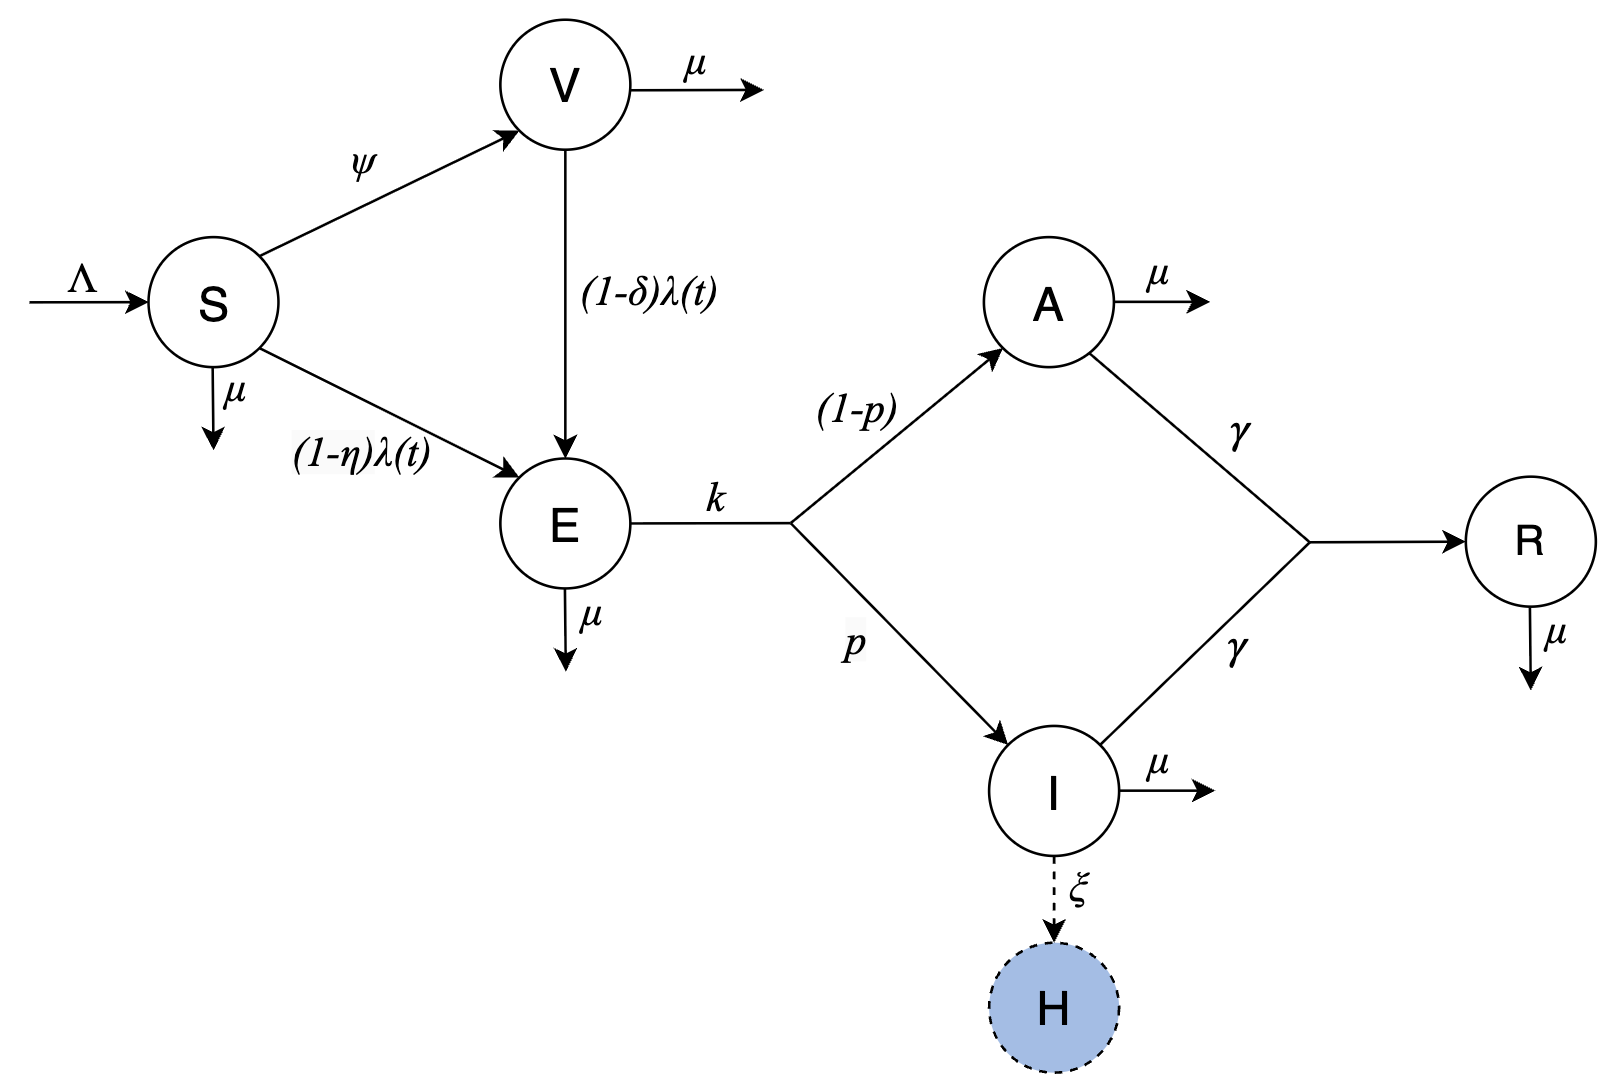
\includegraphics[width=.95\columnwidth]{figures/sveair-h.png} % Slightly narrower than full column
% \vspace{-2mm}
\caption{SVEAIR compartmental model with vaccination and masking. The `H' is not a separate compartment but denotes observed hospitalization numbers, typically a fraction of the true numbers from the infected compartment.}
\label{fig:sveair}
\vspace{-3mm}
\end{figure}


\paragraph{Realistic assumptions for vaccination and masking.}
In the weekly interactive loop between individuals and the PHA (see details in Appendix~\ref{supp:weekly-loop}), masking compliance is defined based on self-reported frequency over the prior 5--7 days, classifying ``all of the time'' or ``most of the time'' as masking and other responses as non-masking, consistent with large-scale survey practice~\cite{spatiotemporal}. To account for the distinctions of vaccination and masking behaviours, the deception rates are pre-specified as 5-15\% and 40-80\%, respectively~\cite{kenya2021,Archambault2023}. 

\paragraph{Signaling game.}
%For notational convenience, we may omit the time index $t$; however, time dependency is understood to be implicit in the formulation.

For the signaling game $\mathcal{G}$, individuals communicate messages from a set $\mathcal{M}$, representing vaccination and masking status.
We encode messages as two bits $b_1b_2$, where $b_1=0$ ($1$) indicates ``Vaccinated'' (``Unvaccinated''), and $b_2=0$ ($1$) indicates ``Masking'' (``Not Masking'').
Thus, the message space is $\mathcal{M}=\{00,01,10,11\}$.
Note that $0$ denotes desirable behavior (i.e., desired by the PHA) on the part of individuals.
We define an individual's behavioral type as $\theta_i=(\theta_i^v,\theta_i^m)\in\Theta$, where $\Theta=\{00,01,10,11\}$, $\theta_i^v$ denotes the true vaccination status, and $\theta_i^m$ denotes the true masking status. For example, $\theta_i=01$ indicates that an individual is vaccinated but does not mask.

Reported messages may, of course, not match actual behavior, e.g., an unvaccinated or non-masking individual may claim otherwise, allowing the
capture of deception. 
The sender strategy is therefore represented by $g(m_i\mid \theta_i)$, which denotes the probability that an individual with true behavioral type $\theta_i$ communicates message $m_i$.
For truthful individuals, $g(m_i=\theta_i\mid\theta_i)=1$, while deceptive individuals may choose messages that provide higher individual utility.
%While we restrict attention to vaccination and masking, the framework generalizes to richer behavioral states.

% Futher, we assume that only $M \leq K$ individuals in group $\mathcal{K}$ report their status. Individual types are represented by $\boldsymbol{c} = [c_1,\cdots,c_K]^T$, where $c_i=1$ denotes honesty and $c_i=0$ indicates deception. Let $g(m\mid c)$ denote the probability of sending message $m$ given type $c$. Since persistent dishonesty reduces payoffs (via penalties and social costs), deceptive individuals adopt probabilistic strategies balancing truth and misreporting. The receiver, in turn, forms beliefs about $\boldsymbol{c}$ to update the epidemiological model (Appendix~\ref{supp:epi_model}), where $\widehat{\psi}$ and $\widehat{\eta}$ denote estimated vaccination and contact rates, respectively. We now define sender and receiver payoffs.
We assume that only a subset of individuals $\mathcal{K}_c\subseteq\mathcal{K}$ responds to PHA survey, while the remaining individuals $\mathcal{K}_s=\mathcal{K}\setminus\mathcal{K}_c$ do not provide behavioral information. Then PHA forms posterior beliefs over behavioral types $q(\theta_i\mid m_i)$, which are used to estimate population-level behavioral parameters, including the vaccination rate $\widehat{\psi}$ and masking rate $\widehat{\eta}$.

\paragraph{Sender utility function.} Falsely claiming to be vaccinated may offer incentives, such as earning more in the workplace. Similarly, falsely stating compliance with mask-wearing may help avoid penalties imposed by the PHA. In short, while honesty about individual actions may support the societal goal of achieving zero infection rates, it could negatively impact individual payoffs. Let $I_v$ and $I_m$ denote the incentives associated with falsely claiming vaccination and masking compliance, respectively.
The sender utility is defined according to the reported message:
\begin{equation}
U_s = \sum_{k\in\mathcal K} U_s^{(k)}(\theta_k,m_k),
\label{eq:utility}
\end{equation}
where the individual-level utility is given by
% % \begin{equation}
% % \begin{aligned}
% % U_s^{(k)}(c_k, m_k) &= g\big(m_k = \text{``00''} \mid c_k = 0\big)(I_v + I_m) \\
% % & +\; g\big(m_k = \text{``01''} \mid c_k = 0\big) I_v \\
% % & +\; g\big(m_k = \text{``10''} \mid c_k = 0\big) I_m.
% % \end{aligned}
% % \label{eq_sender_payoff}
% % \end{equation}

% \begin{equation}
% \begin{aligned}
% U_s^{(k)}(\theta_k,m_k)
% =& 
% g(m_k=00\mid\theta_k)
% \left(
% \mathbf{1}(\theta_k^v=1)I_v + \mathbf{1}(\theta_k^m=1)I_m
% \right)
% \\
% &+
% g(m_k=01\mid\theta_k)
% \mathbf{1}(\theta_k^v=1)I_v
% \\
% &+
% g(m_k=10\mid\theta_k)
% \mathbf{1}(\theta_k^m=1)I_m .
% \end{aligned}
% \label{eq_sender_payoff}
% \end{equation}


\begin{equation}
\begin{aligned}
U_s^{(k)}(\theta_k) = 
\sum_{m_k\in\mathcal M}
g(m_k\mid\theta_k)
\Delta(\theta_k,m_k),
\end{aligned}
\label{eq_sender_payoff}
\end{equation}

and
\begin{equation}
\begin{aligned}
\Delta(\theta_k,m_k)
=&
I_v \mathbf{1} (\theta_k^v=1, m_k^v=0) \\
& + I_m \mathbf{1}(\theta_k^m=1, m_k^m=0)
\end{aligned}
\label{eq:lie_gain}
\end{equation}
denotes the incentive obtained from falsely claiming compliance.

% \begin{equation}
% \begin{aligned}
% U_s^{(k)}(\theta_k)
% =
% \sum_{m_k\in\mathcal M}
% g(m_k\mid\theta_k)
% \Big[
% &I_v\mathbf{1}(\theta_k^v=1,m_k^v=0)
% \\
% &+
% I_m\mathbf{1}(\theta_k^m=1,m_k^m=0)
% \Big].
% \end{aligned}
% \label{eq_sender_payoff}
% \end{equation}

% \noindent
Here, to compute the utility, which is the incentive upon deceiving, we consider only individuals who are either not vaccinated or have not followed masking guidelines. For instance, \( g(m_k = ``00" \mid \theta_k=``11") \) denotes a scenario where the individual has neither adopted vaccination nor masking, yet falsely communicates that they have. 
%Similarly, \( g(m_k = ``01" \mid c_k=0) \) and \( g(m_k = ``10" \mid c_k=0) \) denotes the scenarios where the individual has not adopted vaccination and masking, respectively, yet falsely communicates that they have.

Maximizing only $U_s^{(k)}(\theta_k)$ leads to a trivial solution where the individuals always choose to be dishonest about their strategies, since that will bring them maximum payoffs. %However, such a strategy 
This leads to increased infection rates, closing down of businesses, and potentially punitive measures by the PHA.
Therefore, the sender in our model is interpreted as \emph{a representative population agent} rather than single strategic individuals. The population consists of a continuum of individuals facing identical incentives but potentially making heterogeneous reporting choices. Accordingly, the sender's strategy $g(m \mid \theta)$ represents a population-level mixed strategy, i.e., the empirical distribution of reports generated by individuals under the same incentive structure. In this way, the sender communication strategies must represent a balance between maximizing $U_s^{(k)}(\theta_k)$ and minimizing these losses. 

We represent the losses as proportional to the negative of semantic accuracy, which is defined as the accuracy with which the receiver interprets the individual types from the messages communicated and written as:
\begin{equation}
U_L(p, q) = -\frac{1}{K} \sum\limits_{i \in \mathcal{K}} \sum\limits_{j \in \mathcal{M}} p_{ij} q_{ji},
\end{equation}
where $p_{ij} = g(m_j \mid \theta_i)$, representing the sender communication strategy, and $q_{ji} = q(\theta_i \mid m_j)$, representing the receiver posterior belief. For non-responsive individuals, we set $p_{ij} = q_{ji} = 0$.
The sender's objective is to find a communication policy $g(m_k \mid \theta_k)$ by maximizing the following objective:
% \vspace{-2mm}

\begin{equation}
\mathcal{P}_1:\left[g(m_k \mid \theta_k)^{\ast}\right]_{\forall k} = \argmax\limits_{g(m_k \mid \theta_k),\, \forall k} \left( U_s - \lambda_1 U_L \right),
\end{equation}
where $\lambda_1$ is a weighting factor that represents an optimal trade-off between maximizing $U_s$ and minimizing $U_L$.


Next, to  understand  the   implications of user    misreporting, we define the control reproduction number $R_c$ as the rate at which a person can pass on the infection. The expression for $R_c$ follows  directly from \cite{ChoiJTB2020}, as
\begin{equation}
    R_c(\psi,\eta) = \underbrace{\frac{\beta k}{(k+\mu)(\gamma + \mu)}}_{R_0}\frac{(1-\delta)\psi + (1-\eta)\mu}{\psi + \mu}.
\label{eq_Rc}
\end{equation} 
A value of $R_c(\psi,\eta)>1$ represents endemic equilibrium, where the disease remains endemic in the population. Here $\beta = \beta_0(p+b(1-p))$  indicates the weighted transmission rate considering both symptomatic and asymptomatic
cases. Eq.~\eqref{eq_Rc} means that as  $R_c(\psi,\eta)$ increases, it may have severe consequences of the functioning of business, schools and other institutions. This will adversely impact the payoffs of each individual, in terms of loss of job or restrictions to the number of employees that can work, thereby reducing their salary or benefits. In practice, the reproduction number can be estimated using the available observations  \cite{ShiArxiv2025} by the PHA, such as hospitalization. 
To capture this effect, we modify the sender utility using a discount factor
\begin{equation}
\begin{aligned}
\widetilde{U}_s^{(k)}(\theta_k)
=
e^{-aR_c(\psi,\eta)}
U_s^{(k)}(\theta_k).
\end{aligned}
\label{eq_sender_payoff_modified}
\end{equation}
where $a$ is a constant economic coefficient controlling the slope of the exponential curve. All subsequent sender payoffs are the discounted form $\widetilde{U}_s^{(k)}$, which we write inline as $e^{-aR_c}I(\theta)$ when only the deception gain of a single type is at issue.
% \begin{equation}
%     \begin{aligned}
%     U_s^{(k)}(\theta_k,m_k) &= g(m_k = ``11"\mid \theta_k) e^{-aR_c(\psi,\eta)}(I_v+I_m) \\ & + g(m_k = ``10"\mid \theta_k)e^{-aR_c(\psi,\eta)}I_{v} \\ &+ g(m_k = ``01"\mid \theta_k) e^{-aR_c(\psi,\eta)}I_m,
%     \label{eq_sender_payoff_modified}
%     \end{aligned}
% \end{equation}
% where $a$ is the economic factor, which is a constant coefficient that controls the slope of  the exponential  curve.
As per Eq.~\eqref{eq_sender_payoff_modified}, higher $R_c(\psi,\eta)$ lowers individual payoffs. Stricter PHA measures thus reflect both rising infection rates and their economic impact on daily life. The modified sender payoffs ensure that sender utility depends not only on individual strategies but also on the PHA's ability to predict and control the epidemic without disrupting normal activities.

%As per \eqref{eq_sender_payoff_modified}, as $R_c(\psi,\eta)$ increases, the individual payoffs reduce. Hence, when the PHA introduces stricter measures, that is indicative of the economic impact due to an exploding infection rate and hence on the day-to-day normal activities of the population. The modified sender payoffs ensure that $U_s^{(k)}$ depends not just on individual strategies but also on whether the PHA is able to accurately predict the evolution of epidemiology and hence bring it under control, without impacting the day to day activities of the population.

% \begin{figure}[t]
% \centering
% \includegraphics[width=.8\columnwidth]{AnonymousSubmission/LaTeX/sg.png}
% \caption{Illustration of signaling games.}
% \label{fig:sg}\vspace{-3mm}
% \end{figure}

\paragraph{Receiver utility function.}
The receiver's objective here is to model accurately the epidemiological ODEs in \eqref{eq_ODE} using the estimated values of $\boldsymbol{\phi}(t) = \{\widehat{\psi}(t), \widehat{\eta}(t), \widehat{\lambda}(t), \widehat{\gamma}(t)$. The estimated ODE by the PHA has the same structure as the ground-truth epidemiological model given in Appendix~\ref{supp:epi_model}. The estimation error will typically be given by $\abs{X(t) - \widehat{X}(t)}^2$ for $X \in {S,V,E,I,A,R}$. However, the PHA cannot compute this error directly due to lack of access to ground-truth ODEs (as noted earlier). Fortunately, it can estimate hospitalizations, which are assumed to be proportional to infections~\cite{FoxPNAS2022}. We therefore model the hospitalization count as:
$H(t) = \xi I(t)$,
where $\xi$ is the infection--hospitalization ratio (IHR).
% The receiver's objective is to minimize this error and thereby ensure that the protection strategies followed by it are enough to control the disease. 
For a given sender type and belief,  the hospitalization prediction error (also called distortion) can be written as:
% \begin{equation}
%     D(t) = \sum\limits_{\boldsymbol{c}} p(\boldsymbol{c} \mid \boldsymbol{m}(t)) 
%     \sum\limits_{\boldsymbol{\theta}(t)} p(\boldsymbol{\theta}(t) \mid \boldsymbol{c}) 
%     \left| H(t) - \widehat{H}(t) \right|^2.\label{eq_error}
% \end{equation}

\begin{equation}
D(t)
=
\sum_{\theta}
q(\theta\mid m(t))
\sum_{\boldsymbol{\phi}(t)}
q(\boldsymbol{\phi}(t)\mid\theta)
\left|
H(t)-\widehat H(t)
\right|^2 .
\label{eq_error}
\end{equation}

This distortion measures the inconsistency between observed hospitalization dynamics and the epidemiological trajectory inferred
from behavioral reports, with
$q(\boldsymbol{\phi}(t)\mid\theta)$ capturing the uncertainty in
epidemiological parameters associated with behavioral type $\theta$.
The receiver seeks beliefs that reduce uncertainty about population
behavior while maintaining bounded epidemiological distortion. Therefore,
the receiver optimization problem is formulated as

\begin{equation}
\begin{aligned}
\mathcal{P}_2:
\quad
\min_{q(\theta\mid m)}
&
\sum_{m}
P(m)\,
\mathrm{KL}\!\left(
q(\cdot\mid m)\,\big\|\,
\tfrac{P(\cdot)P_S(m\mid\cdot)}{P(m)}
\right)
\\
&
+\;\lambda_2
\sum_{\theta,m}
P(m)\,
q(\theta\mid m)\,
D(\theta)
\\
\text{s.t.}
&
\sum_{\theta}
q(\theta\mid m)=1,
\quad
\forall m\in\mathcal M .
\end{aligned}
\label{eq:P2}
\end{equation}

\noindent
$\mathcal P_2$ is relative-entropy regularised inference against the Bayes posterior: the
receiver is penalised for moving away from $P(\theta)P_S(m\mid\theta)/P(m)$ and for placing
mass on behavioural states whose implied epidemic dynamics contradict observed
hospitalisations. Its stationarity condition is
\begin{equation}
q^{*}(\theta\mid m)\;\propto\;P(\theta)\,P_S(m\mid\theta)\,e^{-\lambda_2 D(\theta)},
\label{eq:P2-solution}
\end{equation}
which carries the prior and the sender likelihood through the reference measure. A plain
entropy objective would not: entropy is concave on the simplex, so minimising it over a
convex feasible set attains its optimum at a vertex, giving a degenerate point mass rather
than the Gibbs form in \eqref{eq:P2-solution}. Setting $\lambda_2=0$ recovers the Bayes
posterior exactly.

where $P(m)$ denotes the empirical distribution of observed messages received by the PHA, and $D^*$ represents the maximum tolerable
hospitalization prediction distortion.
Based on the inferred behavioral parameters and the estimated epidemiological dynamics, the PHA updates its intervention recommendations through adaptive correction terms:

\begin{align}
\psi_r(t)
&=
\widehat{\psi}(t)
+
\widetilde{\psi}(t),
\\
\eta_r(t)
&=
\widehat{\eta}(t)
+
\widetilde{\eta}(t).
\label{eq:combined_params}
\end{align}

Here, $\widehat{\psi}(t)$ and $\widehat{\eta}(t)$ represent the vaccination and masking levels inferred from behavioral reports,
respectively. The correction terms
$\widetilde{\psi}(t)$ and $\widetilde{\eta}(t)$ compensate for inference errors by reducing the hospitalization prediction distortion. The
resulting quantities $\psi_r(t)$ and $\eta_r(t)$ are the intervention recommendations issued by the PHA and are used to drive the subsequent epidemic evolution.

To characterize the intervention level required for epidemic control, we derive the herd-immunity vaccination threshold from the controlled reproduction number. Specifically, epidemic control requires $R_c(\psi,\eta)<1$.
Solving Eq.~\eqref{eq_Rc} for the vaccination level yields

\begin{equation}
\psi_{HI}
=
\frac{
\mu
\left(
R_0(1-\eta)-1
\right)
}
{
1-R_0(1-\delta)
},
\label{eq:psi_HI}
\end{equation}

where $1<R_0<\frac{1}{1-\delta}$.
The threshold $\psi_{HI}$ represents the minimum vaccination level
required to suppress transmission under a given masking level $\eta$.



\paragraph{Game solution.}

%Shannon's rate-distortion theory \cite{CoverIT1991} aims to compute the solution to the following problem, which is the transmitter problem here:
%\begin{equation}
%    \mathcal{P}_1: R^{\ast}(D) = \min\limits_{-U\leq -U^{\ast}} \mathbb{I}(\boldsymbol{c};\boldsymbol{m})
%\end{equation}

Given the sender communication strategy, the receiver updates its belief about behavioral types using Bayesian inference. Following the rational speech act (RSA) framework, the receiver posterior is given by
\begin{equation} P_L(\theta\mid m) \propto P_S(m\mid\theta)q(\theta), \label{eq:rsa_listener} 
\end{equation} 
where $q(\theta)$ denotes the prior distribution over behavioral types and $P_S(m\mid\theta)$ represents the sender communication strategy. 
Conversely, given the receiver belief, a pragmatic sender chooses messages according to

\begin{equation} 
P_S(m\mid\theta) \propto e^ {\left( \tau \left(u_s(\theta,m) - \lambda_1 u_L(\theta,m) \right) \right)}, 
\label{eq:rsa_speaker} 
\end{equation} 
where $\tau$ controls the rationality of the sender, $u_s(\theta,m)$ denotes the message-level sender utility, and $u_L(\theta,m)$ denotes the semantic loss associated with inferring behavioral type $\theta$ from message $m$. The equilibrium analysis of Section~\ref{sec:equilibrium} works in the $\tau\to\infty$ limit, where \eqref{eq:rsa_speaker} becomes an exact best response and randomisation survives only at indifference. The mixing probability $\alpha$ analysed there is that randomisation, so the strategy $g^{*}(m\mid\theta)$ used throughout is the deterministic-limit specialisation of \eqref{eq:rsa_speaker} to the two-action choice between truthful reporting and the pooling message.

Given the sender strategy, the receiver posterior is obtained by solving
the constrained inference problem in Eq.~\eqref{eq:P2}. The receiver balances two objectives, i.e., reducing uncertainty in inferred behavioral states and maintaining consistency with observed epidemic dynamics.
The corresponding Lagrangian formulation is

\begin{equation}
\begin{aligned}
\mathcal{L}
=&
\sum_{m}
P(m)\,
\mathrm{KL}\!\left(
P_L(\cdot\mid m)\,\big\|\,
\tfrac{P(\cdot)P_S(m\mid\cdot)}{P(m)}
\right)
\\
&
+\lambda_2
\sum_{\theta,m}
P(m)P_L(\theta\mid m)D(\theta)
+\sum_{m}\nu_m\!\left(\sum_{\theta}P_L(\theta\mid m)-1\right),
\end{aligned}
\label{eq:Lagrangian_receiver}
\end{equation}

where $\lambda_2$ weights epidemiological distortion against fidelity to the Bayes
posterior and $\nu_m$ enforces normalisation. Setting
$\partial\mathcal L/\partial P_L(\theta\mid m)=0$ gives
$\log P_L(\theta\mid m)=\log\bigl[P(\theta)P_S(m\mid\theta)/P(m)\bigr]-\lambda_2D(\theta)+c_m$,
so the receiver posterior is

\begin{equation}
P_L(\theta\mid m)
=
\frac{
P_S(m\mid\theta)P(\theta)
\exp(-\lambda_2D(\theta))
}
{
\sum_{\theta'}
P_S(m\mid\theta')
P(\theta')
\exp(-\lambda_2D(\theta'))
},
\label{eq:posterior_solution}
\end{equation}

where $D(\theta)$ denotes the expected hospitalization prediction distortion associated with behavioral type $\theta$. This posterior preserves information contained in the received message
while down-weighting behavioral types whose implied epidemic dynamics
are inconsistent with observed hospitalization trajectories.


\section{Equilibrium Analysis}
\label{sec:equilibrium}

We characterise the reporting stage at a fixed epidemic state. A non-compliant type
$\theta$ chooses $\alpha_\theta\in[0,1]$, the probability of sending the pooling message
$m^{*}=00$, and reports truthfully otherwise; $\theta_{00}$ is compliant and never
misreports. Write $I(\theta)$ for the deception gain, so $I(\theta_{01})=I_m$,
$I(\theta_{10})=I_v$ and $I(\theta_{11})=I_v+I_m$, and $\pi_\theta$ for the population
share. The semantic payoff is the posterior mass the receiver places on the sender's
\emph{true} type given the message \emph{actually sent}:
\begin{equation}
U(\theta,m)=e^{-aR_c}I(\theta)\,\mathbf 1[m=m^{*},\,\theta\neq\theta_{00}]
            +\lambda_1\,q(\theta\mid m).
\label{eq:sender-utility}
\end{equation}

\paragraph{Indifference function.}
For a non-compliant type $\theta$,
\begin{equation}
F_\theta(\alpha)\;=\;U(\theta,m^{*})-U(\theta,m_\theta)
\;=\;e^{-aR_c(\alpha)}I(\theta)-\lambda_1\bigl[1-q(\theta\mid m^{*};\alpha)\bigr].
\label{eq:indiff}
\end{equation}
Equation~\eqref{eq:indiff} compares the two pure actions between which the sender
randomises, which is the correct object for a mixed-strategy indifference condition. The
sender's payoff is affine in $\alpha_\theta$ with slope $F_\theta$, so $\alpha_\theta=0$ is
optimal iff $F_\theta\le0$, $\alpha_\theta=1$ iff $F_\theta\ge0$, and an interior
$\alpha_\theta$ iff $F_\theta=0$.

Evaluating~\eqref{eq:indiff} at the endpoints gives $q(\theta\mid m^{*})\to0$ as
$\alpha\downarrow0$, since a pooling message is then almost surely sent by another type,
and $q(\theta\mid m^{*})=\pi_\theta$ at $\alpha=1$.

\begin{theorem}[Per-period characterisation]
\label{thm:characterisation}
Fix the epidemic state and a non-compliant type $\theta$ with $I(\theta)>0$ and
$\pi_\theta\in(0,1)$.
\begin{enumerate}
\item \textbf{Separation.} $\alpha^{*}_\theta=0$ is a best response iff
  \begin{equation}e^{-aR_c(0)}I(\theta)\;\le\;\lambda_1.\label{eq:sep}\end{equation}
\item \textbf{Pooling.} $\alpha^{*}_\theta=1$ is a best response iff
  \begin{equation}e^{-aR_c(1)}I(\theta)\;\ge\;\lambda_1(1-\pi_\theta).\label{eq:pool}\end{equation}
\item \textbf{Partial pooling.} An interior $\alpha^{*}_\theta\in(0,1)$ requires
  $F_\theta(\alpha^{*})=0$, hence
  \begin{equation}
  \frac{e^{-aR_c(1)}I(\theta)}{1-\pi_\theta}\;<\;\lambda_1\;<\;e^{-aR_c(0)}I(\theta).
  \label{eq:window}\end{equation}
\end{enumerate}
\end{theorem}

Conditions \eqref{eq:sep}--\eqref{eq:window} are exact. No small-$\alpha$ linearisation of
$R_c$ is used, in contrast to the bound reported in the submitted version.

\begin{corollary}[When partial pooling can exist]
\label{cor:nonempty}
The window \eqref{eq:window} is non-empty if and only if
\begin{equation}
-\ln(1-\pi_\theta)\;<\;a\,\bigl[R_c(1)-R_c(0)\bigr].
\label{eq:nonempty}
\end{equation}
\end{corollary}

Condition~\eqref{eq:nonempty} is interpretable: partial pooling survives only when the
epidemic consequence of pooling rather than separating is large relative to how much a
single type can hide behind the others. A rare type can mix over a wide range of
$\lambda_1$; a type comprising most of the population cannot hide, and the window closes.

\begin{corollary}[Exhaustiveness and multiplicity]
\label{cor:exhaust}
At least one of \eqref{eq:sep}, \eqref{eq:pool}, \eqref{eq:window} holds, so a best
response always exists. If neither \eqref{eq:sep} nor \eqref{eq:pool} holds then
\eqref{eq:window} holds, $F_\theta(0)>0>F_\theta(1)$, and an interior root exists by the
intermediate value theorem. If \emph{both} \eqref{eq:sep} and \eqref{eq:pool} hold then
\eqref{eq:nonempty} fails and pure separation and pure pooling are \emph{both} best
responses.
\end{corollary}

Corollary~\ref{cor:exhaust} resolves the inconsistency in the submitted version, where a
separating equilibrium was asserted in the main text and shown impossible in the appendix.
It also qualifies the selection claim: $\lambda_1$ pins down the regime only when
\eqref{eq:nonempty} holds. When it fails, the stage game admits both extremes.

\begin{theorem}[Existence]
\label{thm:existence}
Fix the epidemic state. If the receiver's belief map and $R_c$ are continuous in $\alpha$,
a per-period equilibrium exists. When the distortion multiplier $\lambda_2=0$ the belief
map is Bayes and the profile is a Perfect Bayesian Equilibrium of the stage game.
\end{theorem}

\begin{proof}
Proofs of Theorem~\ref{thm:characterisation}, Corollaries~\ref{cor:nonempty}
and~\ref{cor:exhaust}, and Theorem~\ref{thm:existence} are in
Appendix~\ref{supp:equilibrium-pooling}.
\end{proof}

\paragraph{Scope.}
Theorems~\ref{thm:characterisation} and~\ref{thm:existence} concern the stage game at a
fixed epidemic state and establish \emph{per-period best responses}. They do not establish
uniqueness: $R_c(\alpha)$ is non-monotone, so $F_\theta$ may cross zero more than once and
\eqref{eq:window} may admit several interior roots. Nor do they establish existence or
uniqueness for the full dynamic game coupling the reporting stage to the SVEAIR system,
which is a separate contribution we do not claim here. When $\lambda_2>0$ the receiver's
beliefs are deliberately distorted away from Bayes, so the solution concept is a
\emph{regularised} reporting equilibrium that coincides with Perfect Bayesian Equilibrium
only at $\lambda_2=0$.

% Departing from extremed pooling equilibrium and idealized separating equilibrium, partial pooling equilibrium is achieved when some individuals are honest while others may engage in deception. In this case, even with some dishonesty, PHA receives partial useful signals and tries to obtain $R_c(\psi,\eta) < 1$ and $\widehat{\psi} > \psi_{HI}$. The key question is: \emph{to what extent can deception be tolerated while still ensuring the epidemic converges to an equilibrium with negligible infections?} We decompose $\mathcal{K}$ into $\mathcal{K}_c$, the set of individuals responding to PHA queries, and $\mathcal{K}_s$, those who remain silent. The deception $\tilde{m}$ can then be characterized as:

% \begin{equation}
% \begin{aligned}
%     \tilde{m} = \frac{1}{2}\sum\limits_{k\in \mathcal{K}_c}\sum\limits_{m_k} g(m_k\mid c_k) \lVert m_k-m_k^{(\ast)} \rVert_H + \frac{1}{2}\sum\limits_{k\in \mathcal{K}_s} 2 \\ 
% = \frac{1}{2}\sum\limits_{k\in \mathcal{K}_c}\sum\limits_{m_k} g(m_k\mid c_k) \lVert m_k-m_k^{(\ast)} \rVert_H+ \abs{\mathcal{K}_s},
% \end{aligned}
% \end{equation}
% \noindent
% where $\lVert m_k-m_k^{(\ast)} \rVert_H$ is the hamming distance between communicated message and the ground truth. Using gradient descent, we optimize $\tilde{\psi}$ as follows:
% \begin{equation}
% \tilde{\psi}_t = \tilde{\psi}_{t-1} + \alpha \nabla_{\tilde{\psi}} D(t) 
% \end{equation}
% The objective is to ensure that 
% $\psi^{\ast} +\tilde{\psi} > \psi_{HI}$. Here, the population strategy that maximizes deception while ensuring $R_c(\psi,\eta) < 1$ can be written as the following problem:
% \begin{equation}
% \begin{aligned}  
% g^{\ast}(\boldsymbol{m}\mid \boldsymbol{c})=\argmax\limits_{g(\boldsymbol{m}\mid\boldsymbol{c}),\tilde{\psi}} \tilde{m}  \\
% \mbox{s.t.}\,\, \psi^{\ast} +\tilde{\psi} > \psi_{HI}
% \end{aligned}
% \end{equation}
% The resulting deception will be $\tilde{m}^{\ast} = \frac{1}{2}\sum\limits_{k\in \mathcal{K}_c}\sum\limits_{m_k} g^{\ast}(m_k\mid c_k) \lVert m_k-m_k^{(\ast)} \rVert_H + \abs{\mathcal{K}_s}$. \\

We decompose the population $\mathcal{K}$ into $\mathcal{K}_c$, the set of individuals responding to PHA queries, and $\mathcal{K}_s$, the set of silent individuals. The aggregate deception level $\tilde m\in[0,1]$ is defined as:
\begin{equation}
\begin{aligned}
    \tilde{m} &= \frac{1}{|\mathcal K|}
\left[\frac{1}{2}\sum\limits_{k\in \mathcal{K}_c}\sum\limits_{m_k} g(m_k\mid \theta_k) \lVert m_k-m_k^{(\ast)} \rVert_H + \frac{1}{2}\sum\limits_{k\in \mathcal{K}_s} 2\right] \\ 
              &= \frac{1}{|\mathcal K|}
\left[\frac{1}{2}\sum\limits_{k\in \mathcal{K}_c}\sum\limits_{m_k} g(m_k\mid \theta_k) \lVert m_k-m_k^{(\ast)} \rVert_H + \abs{\mathcal{K}_s}\right],
\end{aligned}
\end{equation}

where $\lVert m_k - m_k^{(\ast)} \rVert_H$ denotes the Hamming distance between the reported message and the ground-truth behavior.
Using gradient descent, the PHA updates the policy correction term $\tilde{\psi}$ as:
\begin{equation}
\tilde{\psi}_t = \tilde{\psi}_{t-1} - \eta_{step} \nabla_{\tilde{\psi}} D(t),
\end{equation}

where $\eta_{\mathrm{step}}$ is the gradient step size. The same update rule applies to $\widetilde{\eta}$, and the resulting intervention recommendations are constrained to valid ranges.


% \subsubsection*{partial pooling equilibrium.}

% In this case, the deception rate is such that $R_c(\psi,\eta) > 1$. Thus, $\widehat{\psi} < \psi_{HI}$ and the population reaches an endemic equilibrium.  This means that at equilibrium, the infected people reach a constant value regardless of the PHA strategies. By substituting for $I^{\prime}=0, A^{\prime}=0$ and $R^{\prime}=0$ in \eqref{eq_ODE}, the endemic equilibrium can be calculated as 
% \begin{align}
%         E^{\ast} &= \left(V^{\ast},E^{\ast},I^{\ast},A^{\ast},R^{\ast}\right) \nonumber \\
%     &=\left(V^{\ast},\frac{\gamma+\mu}{kp}I^{\ast},I^{\ast},\frac{1-p}{p}I^{\ast},\frac{\gamma}{p\mu}I^{\ast}\right).
% \end{align}

% In the presence of an endemic equilibrium, an individual chooses deception when relative utility of deception is greater than that of being honest. This can be expressed as being deceptive when
% \begin{align}
% U_s^{(k)}(c_k,m_k) > \lambda U_L.
% \label{eq_endemic_eq_condition1}
% \end{align}
% Responding to this scenario, the PHA can choose correction factors $\tilde{\psi}$ and  $\tilde{\eta}$ such that at convergence ( i.e., at   $t=\infty$),  $D(\infty) = \sum\limits_{\boldsymbol{c}} p(\boldsymbol{c} \mid \boldsymbol{m}(\infty)) 
% \sum\limits_{\boldsymbol{\theta}(\infty)} p(\boldsymbol{\theta}(\infty) \mid \boldsymbol{c}) 
%     \left| \xi  I^{\ast} - \widehat{H}(\infty) \right|^2 $ ,   where $\widehat{H}(\infty)$ corresponds  to the   estimated hospitalization rate  under  the maximum  tolerable deception.

\section{Experimental Results}

\paragraph{Experimental settings.}
We simulate $n=100$ Monte Carlo runs of a K=10{,}000-person SVEAIR population over 26 weeks following the two stage loop of individuals reporting and PHA modeling as shown in Figure~\ref{fig:System_Model}.
Experiments span a factorial grid of equilibrium types, policy adaptivity, and experimental settings, evaluated on epidemiological, behavioral, and strategic metrics.
Details about simulation rules and evaluation procedures are provided in Appendix~\ref{supp:settings}.

\paragraph{Interactive feedback between population and PHA drives effective epidemic control.}

To reflect the real-world settings, we consider two regimes: (1) low baseline behavioral rates ($\psi=0.05$, $\eta=0.10$), representing adverse conditions in which protective behaviors are largely neglected, and (2) high baseline behavioral rates ($\psi=0.15$, $\eta=0.15$), corresponding to more favorable conditions.
Figure~\ref{fig:rc} shows the evolution of $R_c$ across equilibria compared against a no-interaction baseline. 
Under low baseline rates (Figure~\ref{fig:rc}a), the separating and partial pooling equilibria achieve epidemic control ($R_c <1$) at week~17 and~24. Pooling fails to reach the epidemic threshold within the simulation horizon, indicating sustained transmission due to severely degraded information quality.
When initial behaviors are better (Figure~\ref{fig:rc}b), all three equilibria achieve control with different speeds: separating (week~5), partial pooling (week~9), pooling (week~18). 
In both scenarios, the no-interaction baseline remains $R_c > 1$, demonstrating that adaptive, behavior-informed feedback between the population and the PHA is essential for maintaining effective epidemic control.

\begin{figure}[tbp]
    \centering
    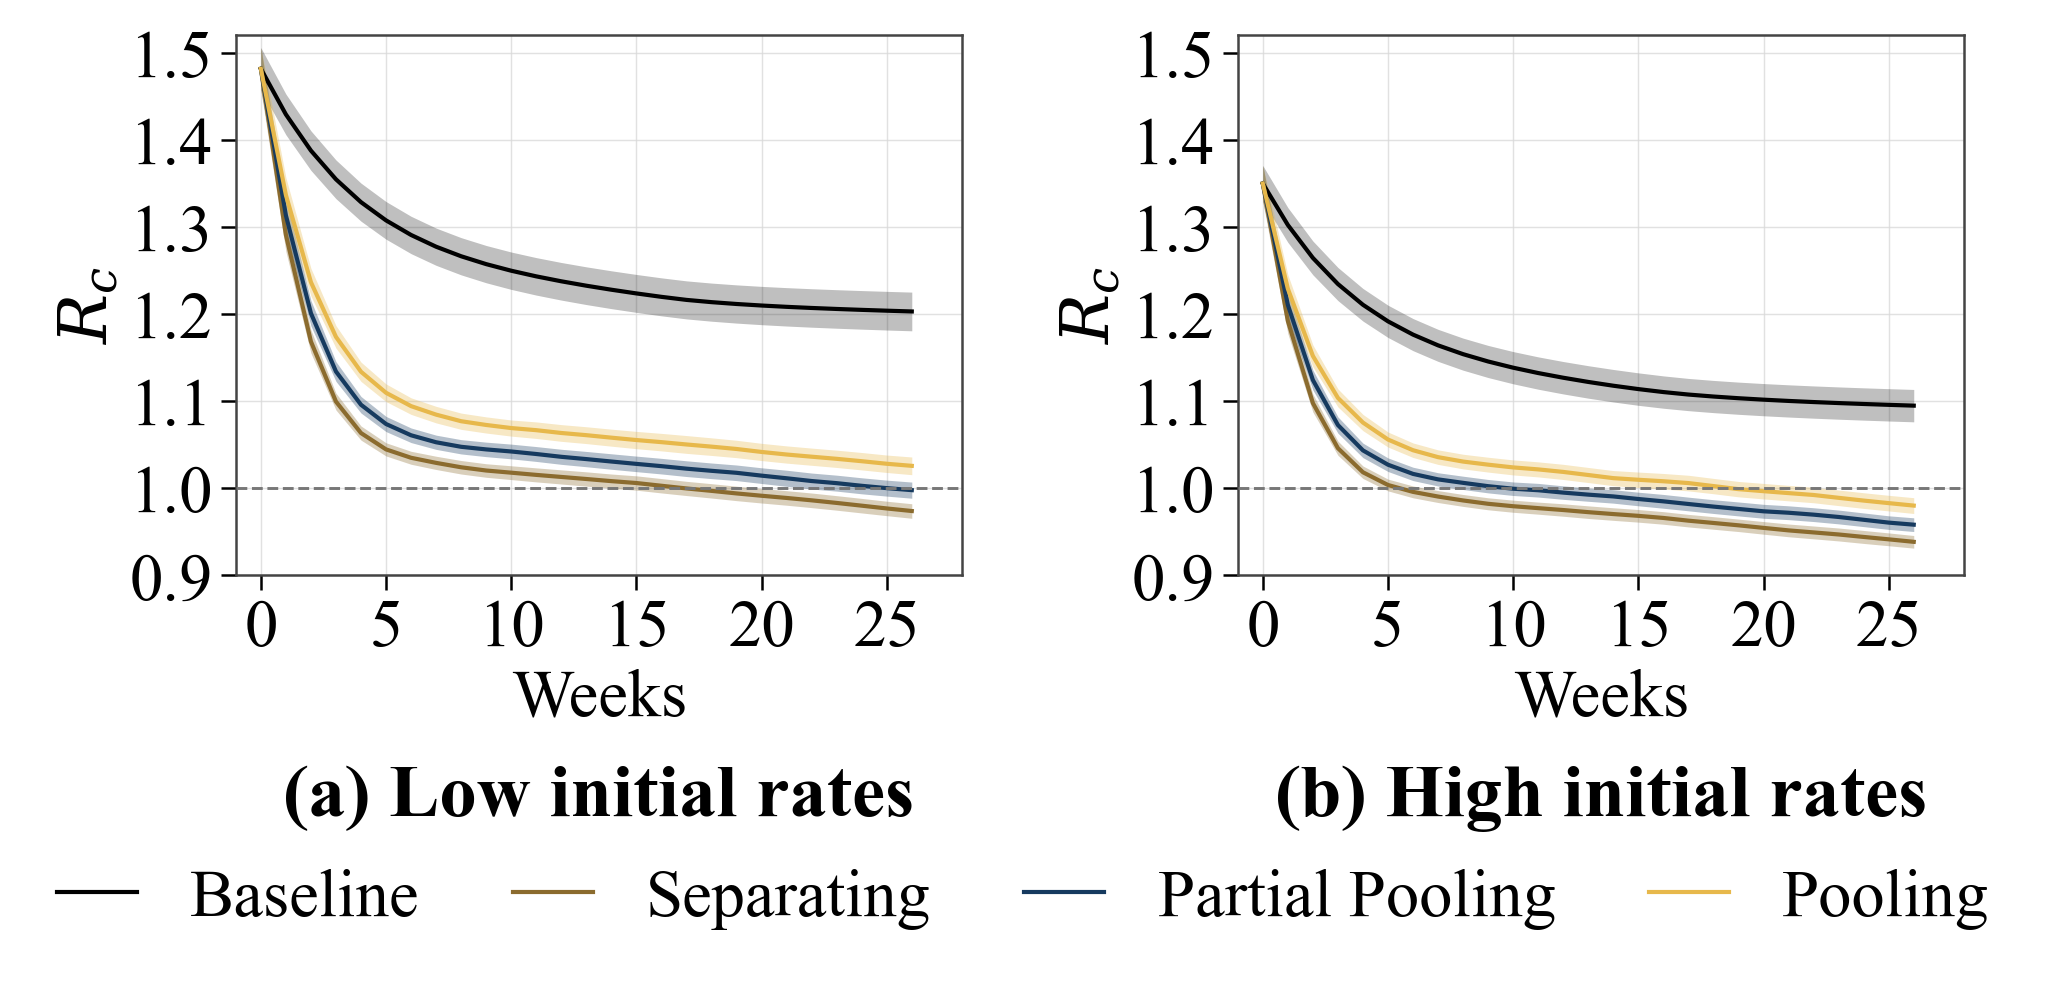
\includegraphics[width=.9\columnwidth]{figures/rc_comparison.png}
    \caption{Controlled reproduction number ($R_c$) across equilibria vs no-interaction baseline with low (a) and high (b) initial behavioral rates.}
    \label{fig:rc} 
    \vspace{-2mm}
\end{figure}


\begin{figure}[tbp]
    \centering
    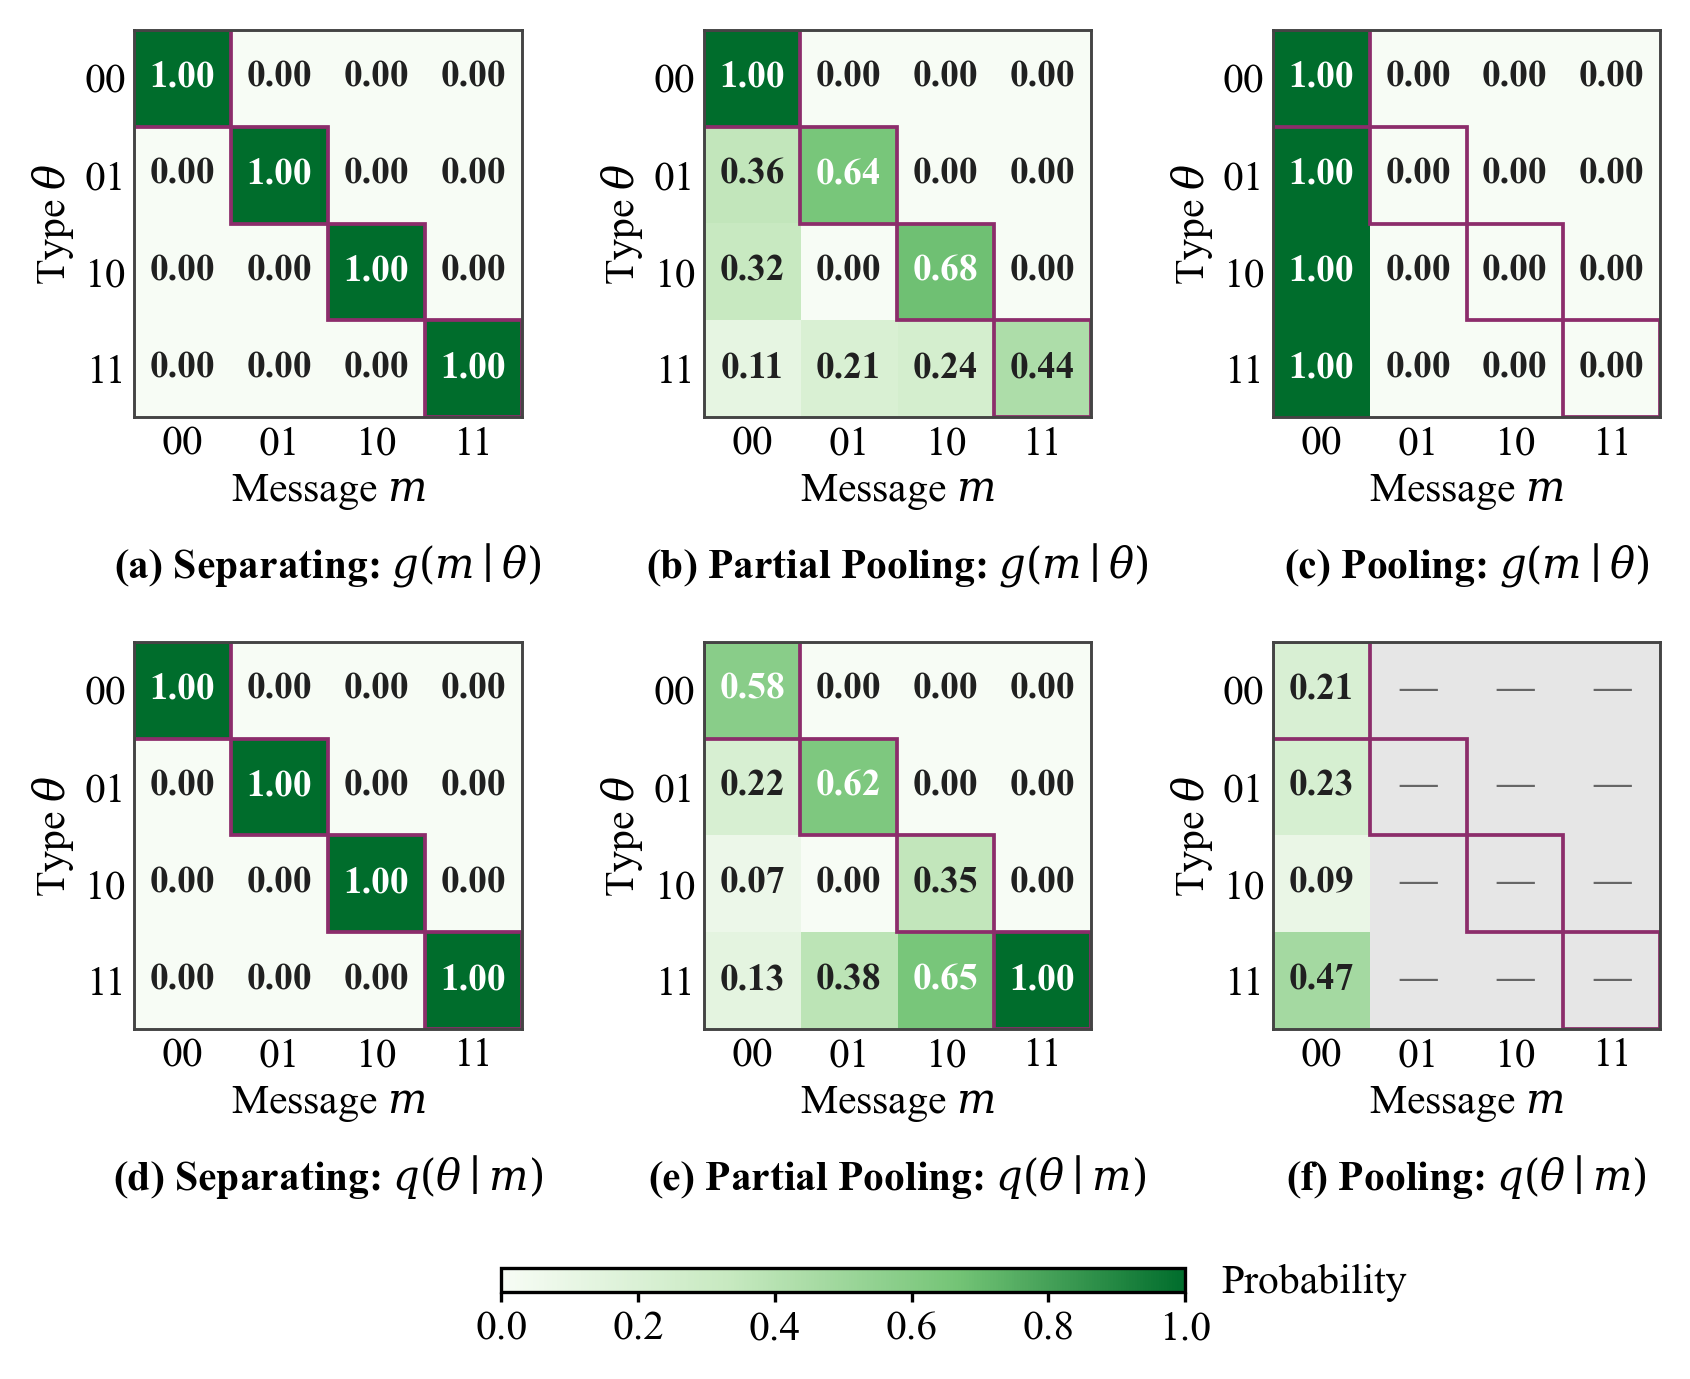
\includegraphics[width=\linewidth]{figures/belief_heatmap.png}
    \caption{Sender strategies $g(m \mid \theta)$ and receiver beliefs $q(\theta \mid m)$ across equilibria.}
    \label{fig:strategy-belief}
    \vspace{-2mm}
\end{figure}


\paragraph{Even imperfect behavioral reports provide informative signals for the PHA}

Figure~\ref{fig:strategy-belief} shows the sender communication strategy $g(m\mid\theta)$ and receiver belief $q(\theta\mid m)$ at the end of the simulation. In the separating equilibrium (Figure~\ref{fig:strategy-belief}a,d), each behavioral type sends a distinct message, allowing the receiver to recover the underlying type distribution with posterior probability one. In contrast, in the pooling equilibrium (Figure~\ref{fig:strategy-belief}c,f), all types send the same message, causing the receiver belief to collapse to the prior and making the behavioral reports uninformative.
The partial pooling equilibrium (Figure~\ref{fig:strategy-belief}b,e) represents an intermediate information regime. Although strategic misreporting introduces ambiguity between behavioral types, the received signals remain partially informative, enabling the receiver to recover non-trivial posterior beliefs. These results show that even imperfect behavioral reports can provide actionable information for the PHA, while the equilibrium structure determines the extent to which such information can be extracted.


\paragraph{Signaling game equilibria govern persistent deception patterns.}

The overall deception rate and separate deception rates for vaccination and masking are shown in Figure~\ref{fig:deception_low} and Figure~\ref{fig:deception_high}. Under low baseline rates (Figure~\ref{fig:deception_low}), pooling exhibits the highest deception: the overall deception rate starts above 0.8 and gradually declines toward about 0.65 by week 26. Partial pooling has intermediate deception, decreasing from 0.6 to 0.5, while separating maintains the lowest and most stable deception around 0.3 (reflection of non-responsive share). 
%Within each equilibrium, masking deception (dotted curves) is consistently higher than vaccination deception (dashed curves), indicating that individuals are more easily misreport masking.
The same ordering persists when baseline rates are high (Figure~\ref{fig:deception_high}). 
%Partial pooling shows a pronounced decline in masking deception, falling from above 0.5 to near 0.35 by week 26. Separating remains 0.3. 
These results highlight that equilibrium structure dominates the level of dishonesty, and that higher initial behavioral rates modestly reduces deceptive reporting.

\begin{figure}[tbp]
    \centering
    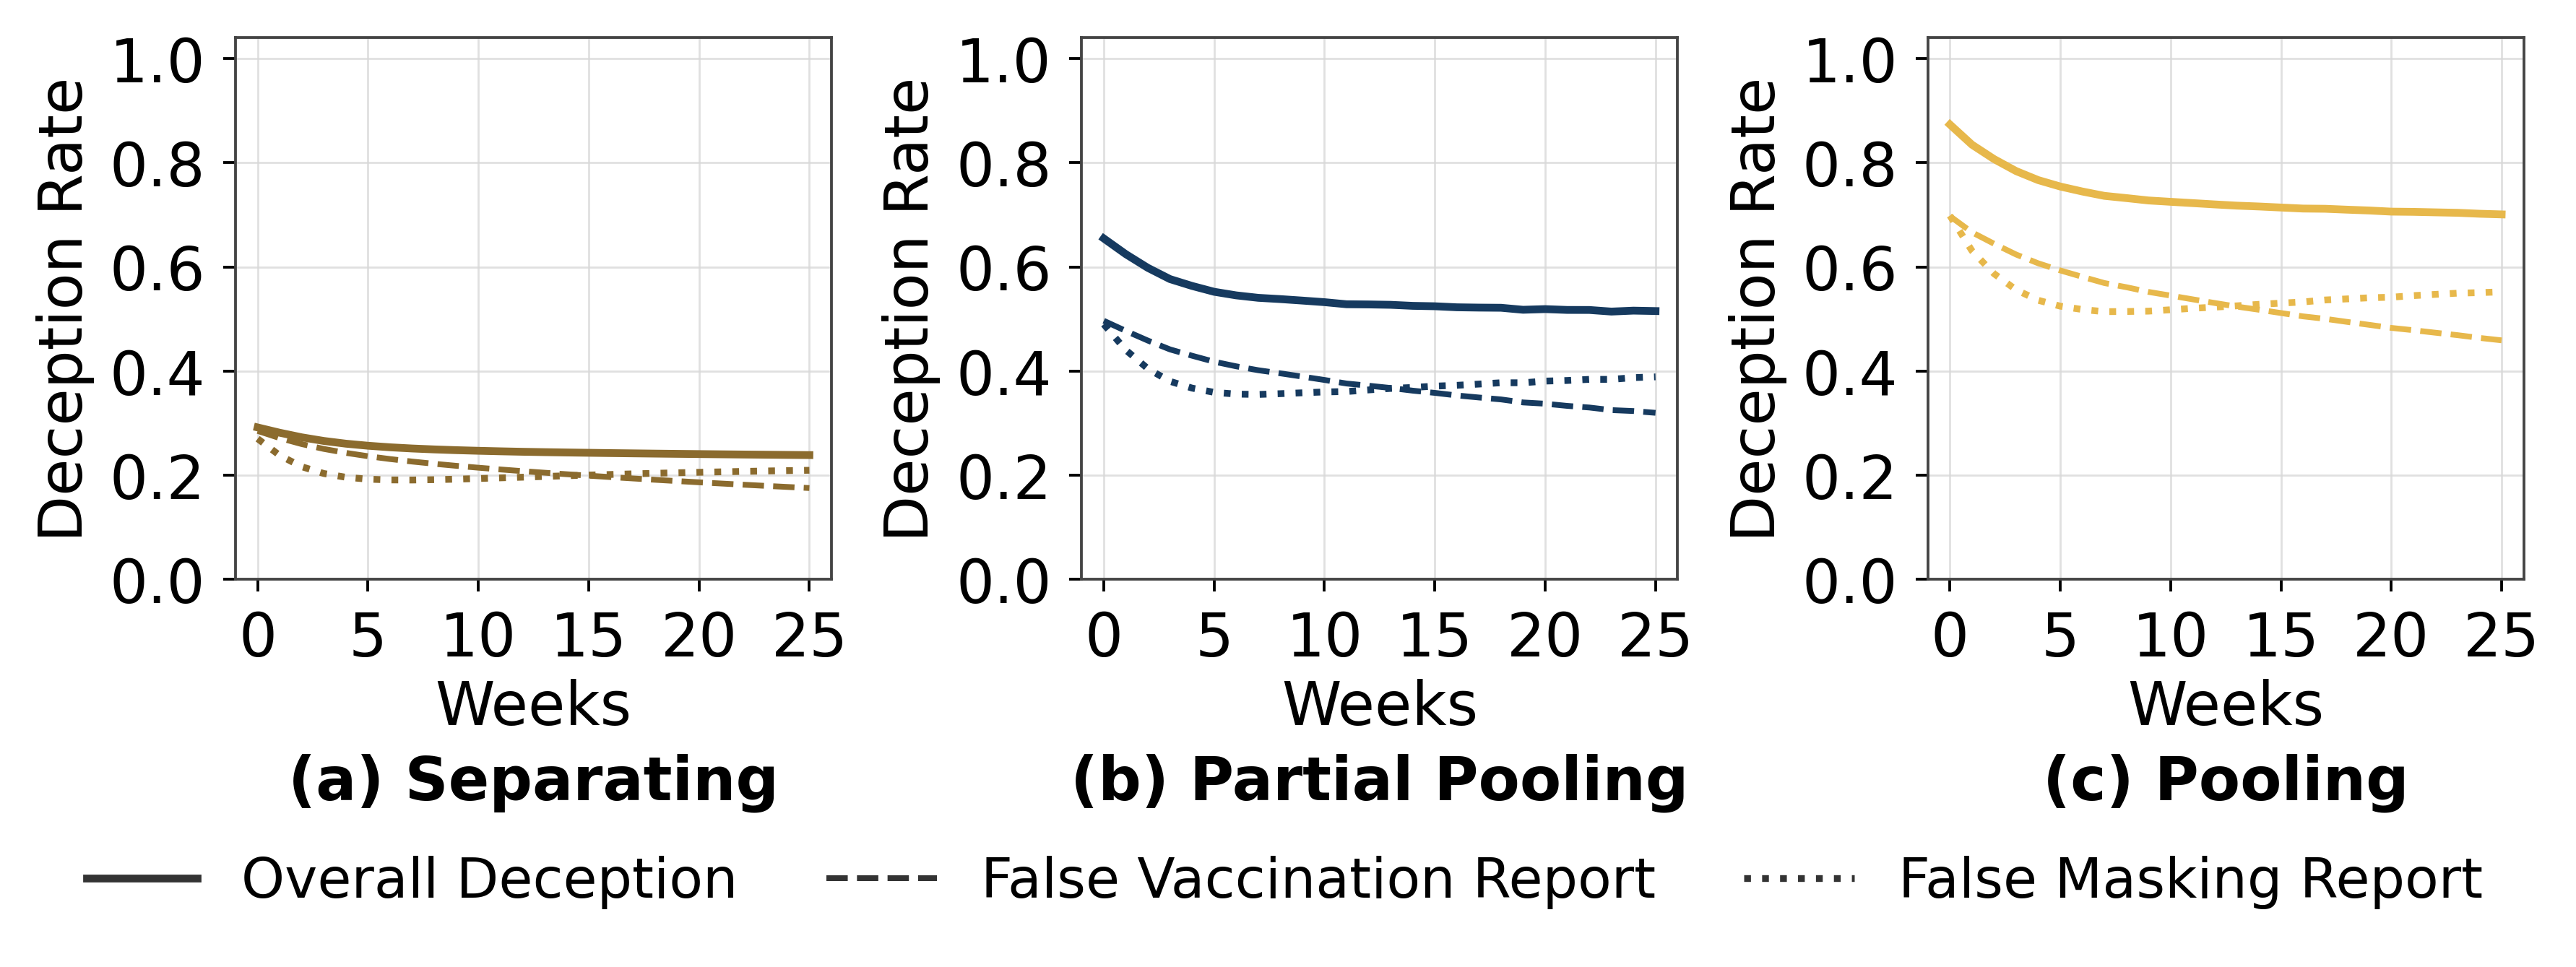
\includegraphics[width=\linewidth]{figures/deception_all-equilibria_low.png}
    \caption{The deception rates across equilibria under low initial behavioral rates.}
    \label{fig:deception_low}
    \vspace{-2mm}
\end{figure}


\begin{figure*}[tp]
    \centering
    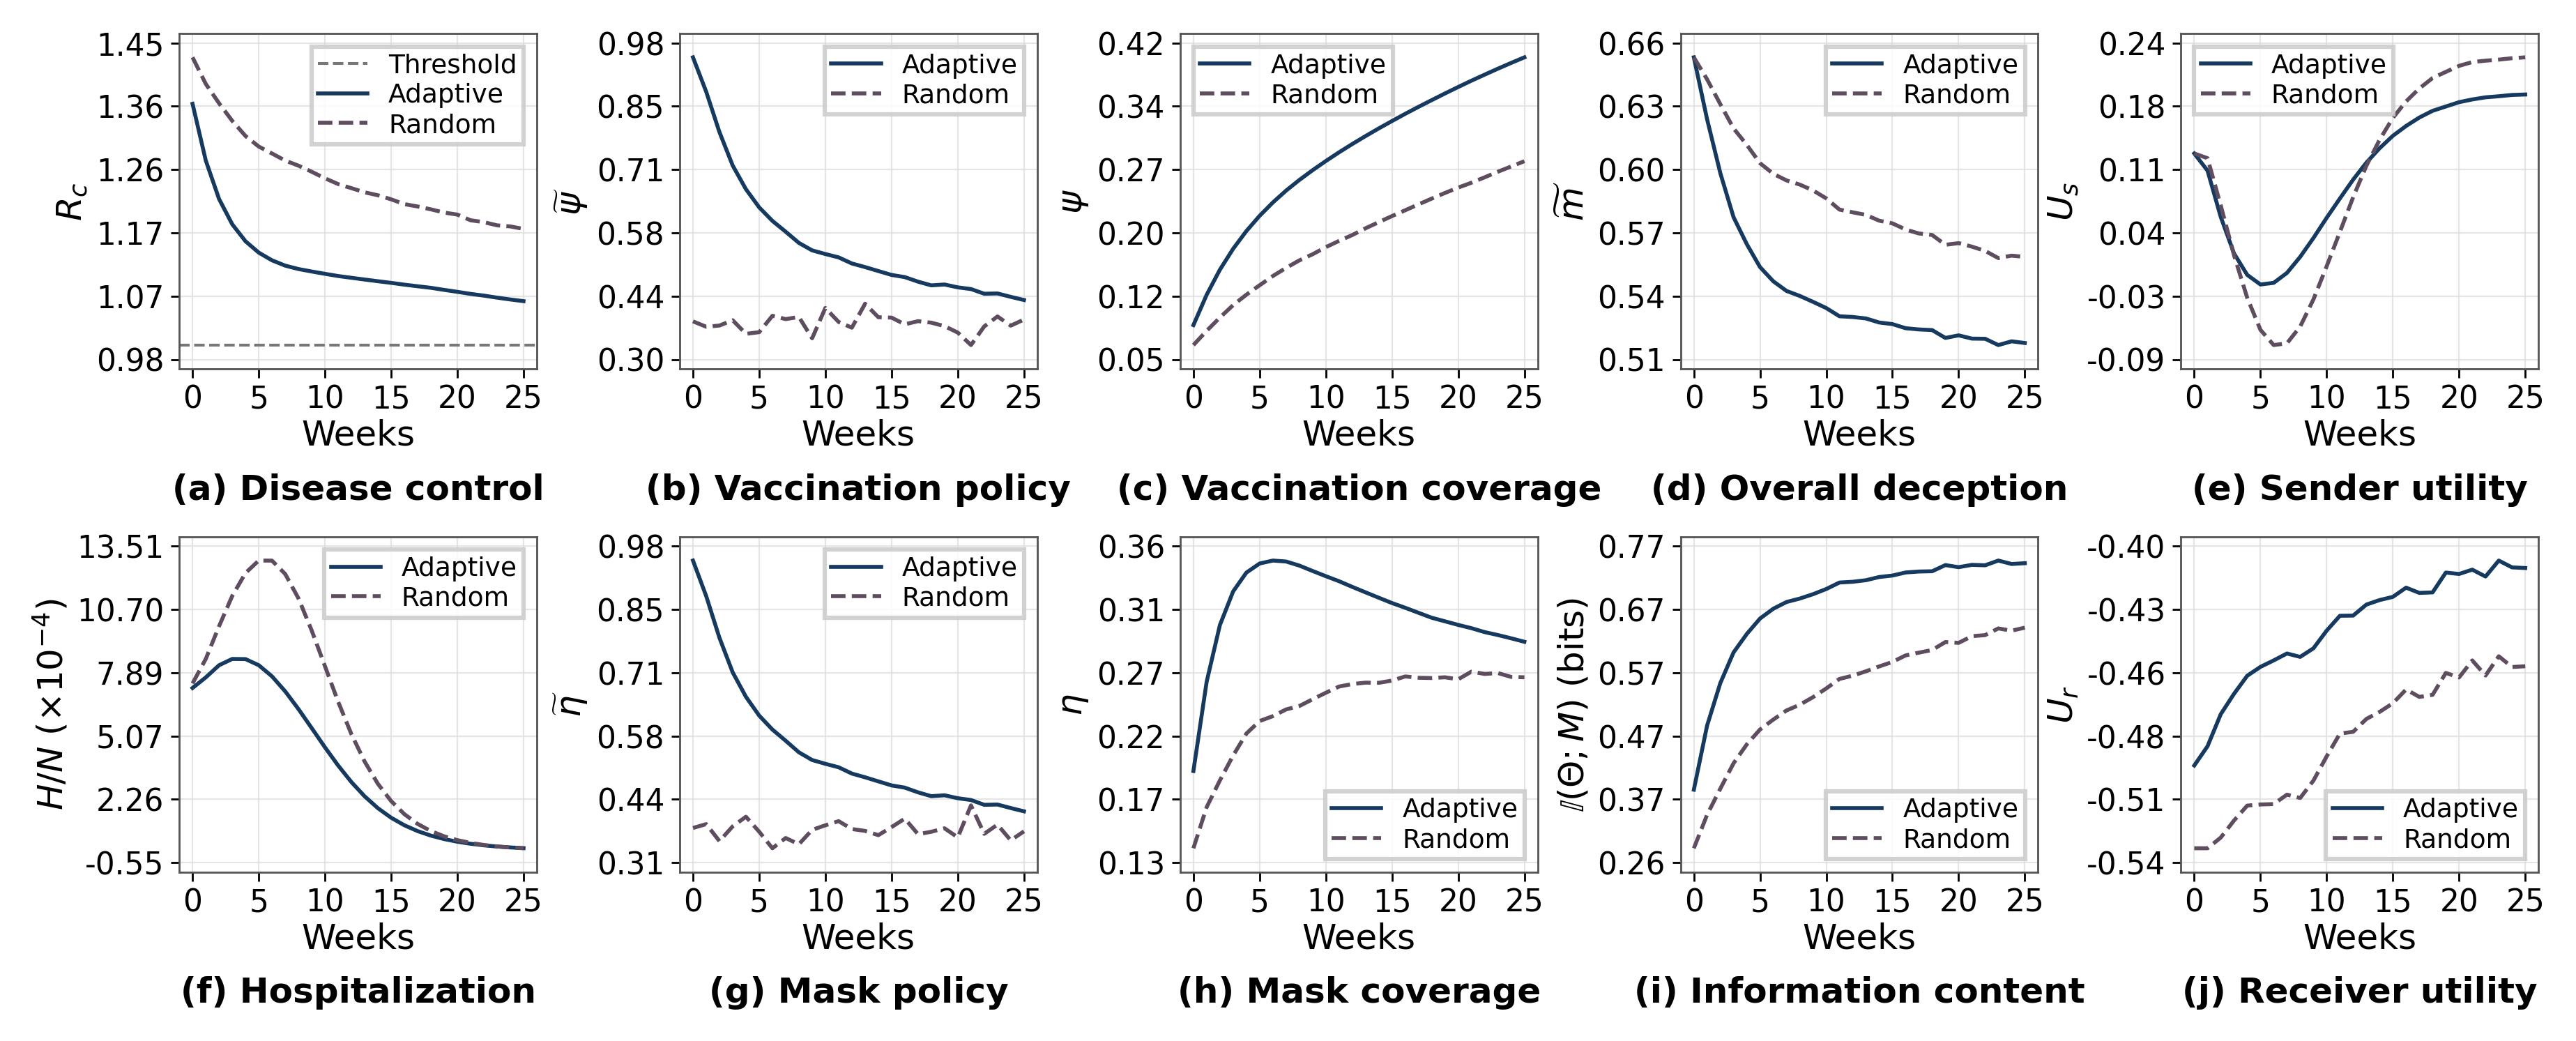
\includegraphics[width=\textwidth, height=4.7cm]{figures/policy_partial_pooling_low}
    \caption{Comparison of adaptive and random policies under partial pooling with low initial behavioral rates, across epidemic dynamics, policy actions, signaling behavior, and utilities.}
    \label{fig:gov_policy_partial_low} %\vspace{-4mm}
\end{figure*}

\paragraph{Adaptive, signal-informed policy supports epidemic mitigation.}

To quantify the value of behavioral information, we benchmark our adaptive, signal-informed PHA response against a random policy that ignores the information of reports under partial pooling with low initial behavioral rates. 
Under the adaptive policy, $R_c$ falls below one at week 22, associated with lower peak hospitalization (0.0037 vs 0.0058) (Figure~\ref{fig:gov_policy_partial_low}a,~\ref{fig:gov_policy_partial_low}f); whereas under the random policy disease not controlled.
Adaptive feedback drives vaccination and masking intensity near their caps between weeks 3--10 (Figure~\ref{fig:gov_policy_partial_low}b,~\ref{fig:gov_policy_partial_low}g), producing rapid gains in coverage to roughly 60\% by week 10, compared to below 20\% under random control (Figure~\ref{fig:gov_policy_partial_low}c,~\ref{fig:gov_policy_partial_low}h); despite higher early deception, the overall deception rate plateaus at $0.4$ vs a stable $\sim0.5$ under random policy (Figure~\ref{fig:gov_policy_partial_low}d), and more rapid growth of information content bits grow much faster, indicating more informative signals received by the PHA (Figure~\ref{fig:gov_policy_partial_low}i). Sender utility rises more under adaptive control (from 0.24 to 0.34) than under random (0.31), and receiver utility is markedly higher, peaking near 6 versus staying below 1.5 (Figure~\ref{fig:gov_policy_partial_low}e,~\ref{fig:gov_policy_partial_low}j). Similar patterns across equilibria and initial compliance are shown in Appendix~\ref{supp: policy_comparison}, where the overall quality of control follows the expected ordering separating $>$ partial pooling $>$ pooling.


\paragraph{Partial pooling quantifies the tolerance frontier between behavioral deception and epidemic control.}

\begin{figure}[tbp]
\centering
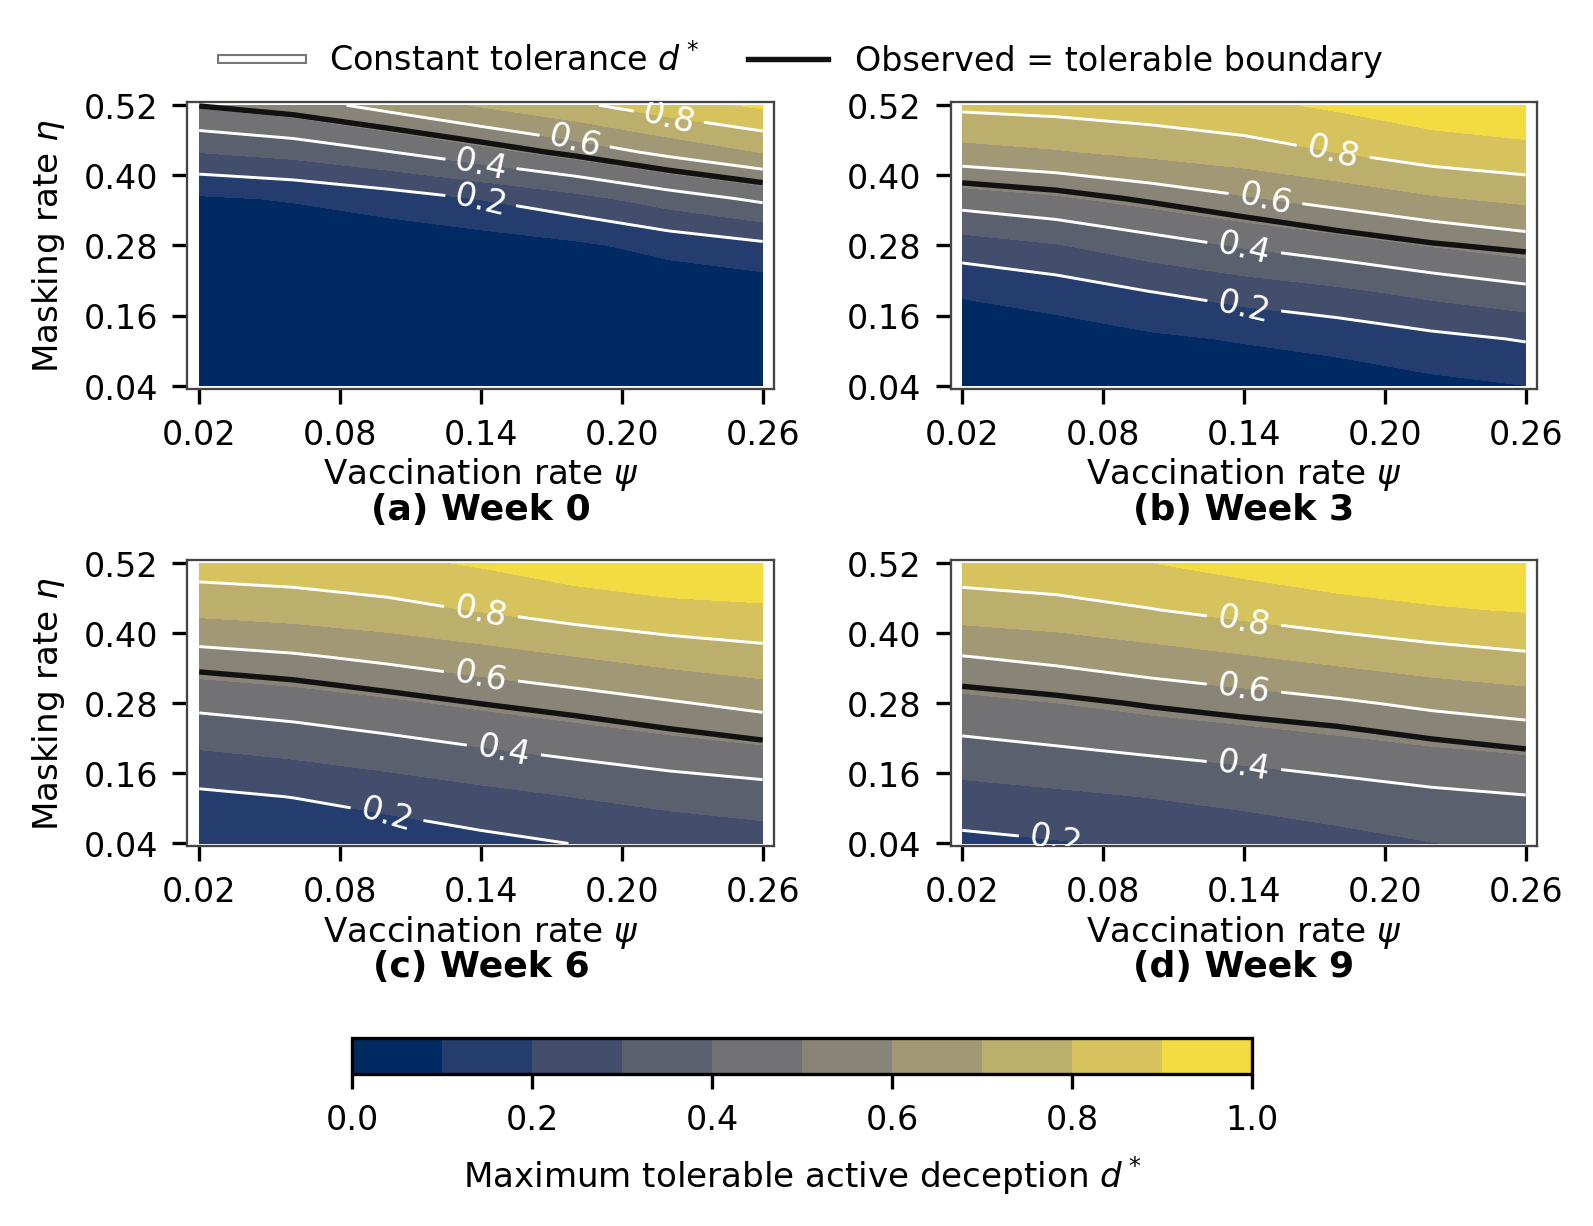
\includegraphics[width=\columnwidth]{figures/tolerance.png} 
\vspace{-2mm}
\caption{Maximum tolerable active deception under partial pooling across epidemic stages.}
\label{fig:tolerance_contours}% \vspace{-4mm}
\end{figure}

Figure~\ref{fig:tolerance_contours} characterizes the maximum tolerable active-deception level $d^*$ under partial pooling across combinations of vaccination rate $\psi$ and masking rate $\eta$. At Week~0, tolerance is limited when both behavioral rates are low but increases substantially as vaccination and masking coverage rises. The black curve marks combinations at which observed deception equals the tolerable level; regions above this boundary provide a positive tolerance margin. Across Weeks~3, 6, and 9, the tolerable region expands and the equality boundary shifts toward lower behavioral rates. Thus, under the modeled trajectory, the system becomes more robust to deception as behavioral protection accumulates and epidemic pressure is increasingly controlled. This pattern should not be interpreted as evidence that information quality becomes unimportant: low-coverage combinations continue to provide the smallest tolerance margins, particularly early in the outbreak. The contours also indicate complementarity between vaccination and masking. Higher adoption of either intervention can partly compensate for lower adoption of the other, although combinations with high values of both provide the greatest robustness to strategic misreporting. Overall, the figure quantifies how the behavioral protection profile and epidemic stage jointly determine the level of active deception that can be accommodated under the specified control criterion.


\begin{figure}[tbp]
    \centering
    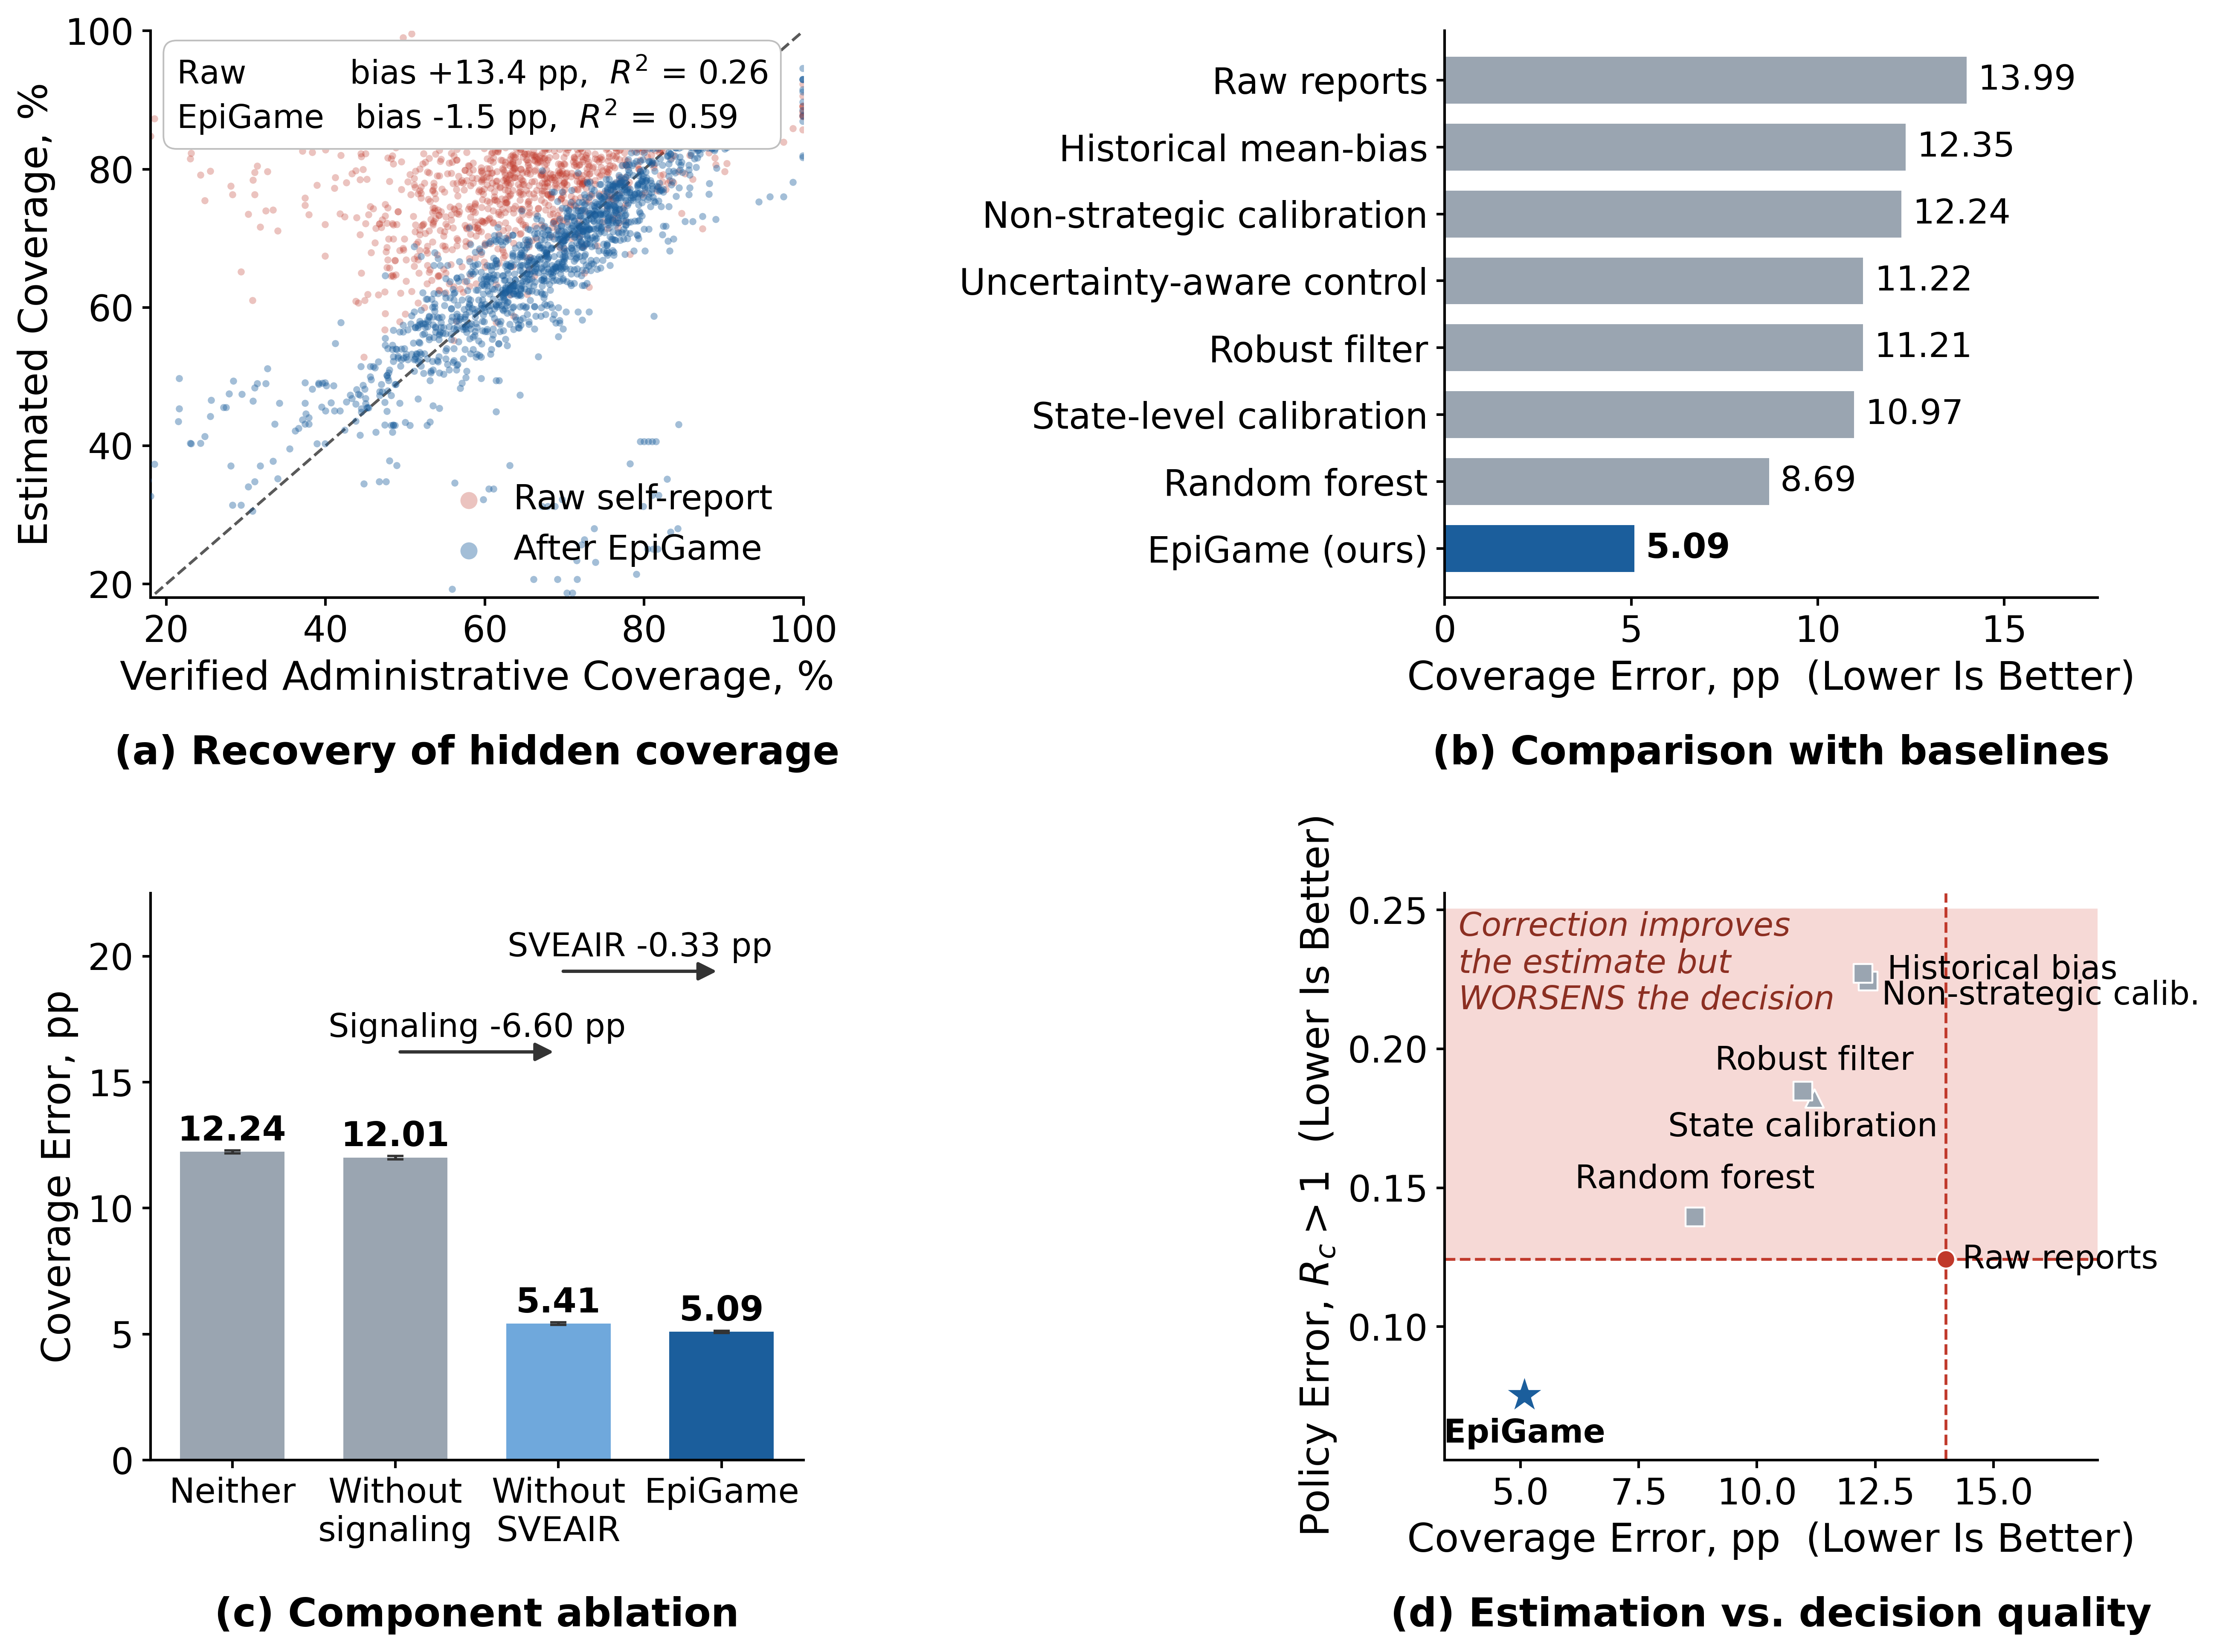
\includegraphics[width=\columnwidth]{figures/real_case.png}
    \caption{Real-world behavioral-state recovery and policy classification
    on held-out CTIS--CDC county-weeks.}
    % Shading marks improved coverage estimation but worse policy classification than raw reports.
    % Error bars show $\pm1.96$ standard errors over 30 paired audit draws.}
    \label{fig:real_case}
    \vspace{-3mm}
\end{figure}

% \paragraph{Real-world evidence supports strategic behavioral distortion modeling}
\paragraph{Real-world evaluation supports policy-relevant behavioral inference}
To examine whether real-world behavioral distortions exhibit the strategic structure assumed by \model{}, we evaluate CTIS self-reported vaccination against matched CDC adult administrative coverage across 10,039 county-weeks from 546 counties in 48 states. The 3,531 county-weeks after August 11, 2021 are held out, and only 25\% of training observations are audited. All methods use identical available inputs and splits, with ridge penalties selected on inner training splits. Correction reduces coverage bias from $+13.4$ to $-1.5$ percentage points (pp) and increases $R^2$ from $0.26$ to $0.59$ (Figure~\ref{fig:real_case}a). \model{} achieves the lowest coverage error at $5.09$ pp, compared with $13.99$ pp for raw reports and $8.69$ pp for the strongest alternative, random forest (Figure~\ref{fig:real_case}b). Removing the signaling component increases error to $12.01$ pp, while removing the SVEAIR consistency constraint increases it to $5.41$ pp (Figure~\ref{fig:real_case}c). Several corrections improve coverage estimates but worsen classification of $R_c>1$, whereas the coupled framework improves both outcomes under the common epidemiological mapping (Figure~\ref{fig:real_case}d). These results support integrating reporting correction with epidemiological structure for policy-relevant inference.  Figure~\ref{fig:real_case} reports (a) reported and corrected coverage against CDC records, (b) coverage error across baselines, (c) \model{} component ablations, and (d) coverage against policy error.

\begin{table}[tbp]
\centering
\caption{Separate control experiment on held-out CTIS--CDC
county-weeks. Lower error is better. }
\label{tab:control-comparison}
\vspace{-2mm}
\small
\setlength{\tabcolsep}{3pt}
\renewcommand{\arraystretch}{1.02}
\begin{tabularx}{\columnwidth}{
@{}
>{\raggedright\arraybackslash}X
rrr
@{}}
\toprule
Method
& \shortstack{Policy error}
& \shortstack{Intervention rate}
& \shortstack{Fixed-budget error} \\
\midrule
Raw reports
& \underline{0.1243} & \textbf{0.0006} & 0.1597 \\
Robust filter
& 0.1860 & 0.1730 & \underline{0.1547} \\
Uncertainty control
& 0.6597 & 0.6236 & 0.2417 \\
\model{}
& \textbf{0.0778} & \underline{0.1260} & \textbf{0.0779} \\
\bottomrule
\end{tabularx}
\vspace{1mm} \parbox{\columnwidth}{ \footnotesize \textit{Note:} Intervention rate is the fraction of county-weeks flagged for intervention.
Fixed-budget error is a retrospective diagnostic that evaluates score rankings at a common budget equal to the observed held-out exceedance count.}
\vspace{-5mm}
\end{table}

Table~\ref{tab:control-comparison} distinguishes estimation quality from intervention intensity. The framework achieves lower policy-classification error than the filtering and uncertainty-aware alternatives. The retrospective fixed-budget comparison additionally evaluates whether their scores prioritize the county-weeks requiring intervention. These results support integrating reporting correction with epidemiological structure for policy-relevant behavioral inference. Complementary individual-level validation uses paired household vaccination reports and provider records from NIS-Teen (Table~\ref{tab:nis-teen-validation}).

\paragraph{Performance depends on the reporting mechanism.}
We evaluate \model{} using CDC vaccination and HHS
hospitalization trajectories with controlled semi-synthetic
reporting distortions.
Under risk-dependent, persistent, and coordinated distortions,
\model{} reduces vaccination-state error by approximately
68\%, 34\%, and 21\%, respectively, relative to the best
alternative in each setting (Table~\ref{tab:mechanism-benchmark}).
Under mean-zero random error, its error is close to that
of raw reports, whereas drifting bias favors raw reports.
These results identify the reporting mechanisms under which
structured correction improves recovery and those under
which it offers limited benefit or increases error.

\begin{table}[tbp]
\centering
\caption{Vaccination-state error under semi-synthetic reporting distortions. Lower is better. }
\label{tab:mechanism-benchmark}
\vspace{-2mm}
\small
\setlength{\tabcolsep}{2pt}
\renewcommand{\arraystretch}{0.95}

\begin{tabularx}{\columnwidth}{
    @{}
    >{\raggedright\arraybackslash}p{0.24\columnwidth}
    *{5}{>{\centering\arraybackslash}X}
    @{}
}
\toprule
Method
& \shortstack{Risk-dep.}
& Persistent
& Coordinated
& \shortstack{Drifting}
& \shortstack{Random} \\
\midrule
Raw reports
& 0.0660
& 0.0479
& \underline{0.0378}
& \textbf{0.0133}
& \textbf{0.0351} \\

Historical mean
& \underline{0.0405}
& \underline{0.0290}
& 0.0714
& 0.0591
& \underline{0.0353} \\

Non-strategic
& 0.0747
& 0.0649
& 0.0967
& 0.0879
& 0.0610 \\

Random forest
& 0.0464
& 0.0399
& 0.0574
& 0.0593
& 0.0450 \\

\model{}
& \textbf{0.0128}
& \textbf{0.0190}
& \textbf{0.0299}
& \underline{0.0328}
& \underline{0.0353} \\
\bottomrule
\end{tabularx}
% \vspace{-5mm}
\end{table}



\paragraph{Robustness of \model{} to stress factors across equilibria.}

\begin{table}[tbp]
\centering
\caption{Stress-test outcomes across equilibria. Disease control score shows
changes relative to baseline, while peak hospitalization reports ratios
relative to baseline.}
\label{tab:stress}

\vspace{-2mm}
\small
\setlength{\tabcolsep}{2.5pt}
\renewcommand{\arraystretch}{.95}

\begin{tabular}{@{}lcccccc@{}}
\toprule
& \multicolumn{3}{c}{Disease Control Score ($\Delta$)}
& \multicolumn{3}{c}{Peak Hospitalization (ratio)} \\
\cmidrule(lr){2-4}
\cmidrule(lr){5-7}

Factor 
& Sep.
& Partial
& Pooling
& Sep.
& Partial
& Pooling \\

\midrule

IHR
& 0.065
& 0.046
& 0.028
& 1.993
& 1.985
& 1.975 \\

Incentives
& -0.085
& -0.065
& -0.042
& 1.021
& 1.029
& 1.035 \\

NRS
& -0.263
& -0.188
& -0.117
& 1.120
& 1.144
& 1.163 \\

Vaccine efficacy
& 0.325
& 0.320
& 0.243
& 0.989
& 0.981
& 0.972 \\

\bottomrule
\end{tabular}
\vspace{1mm} \parbox{\columnwidth}{ \footnotesize \textit{Note:} Disease control scores are reported as changes relative to the baseline setting, where positive values indicate improved control. Peak hospitalization values are ratios relative to the baseline peak hospitalization. IHR denotes the infection--hospitalization ratio and NRS denotes the non-responsive share. Sep., Partial, and Pooling denote the separating, partial pooling, and pooling equilibria, respectively. }
\vspace{-5mm}
\end{table}

We perform a series of stress tests to validate our simulation framework under key factors, including infection--hospitalization ratios (IHRs), incentives for vaccination and masking, the non-responsive share (NRS) to surveys, and vaccine efficacy. Table~\ref{tab:stress} summarizes how robust epidemic control is to these perturbations under all equilibria. Differences in disease control scores and ratios of peak hospitalization are reported relative to the baseline setting defined in Table~\ref{tab:param-summary}. As expected, increasing the IHR approximately doubles peak hospitalization across all equilibria (1.975--1.993$\times$ the baseline peak), while producing modest improvements in disease control scores. Increasing vaccine efficacy provides the largest improvement in epidemic control, increasing the disease control score by 0.325, 0.320, and 0.243 under separating, partial pooling, and pooling equilibria, respectively, while slightly reducing peak hospitalization. By contrast, changes in incentives have relatively limited effects on epidemic outcomes, suggesting that moderate variations in behavioral incentives do not substantially alter the long-term control dynamics. Increasing the non-responsive share has a more pronounced negative impact, reducing disease control scores by 0.263, 0.188, and 0.117 across the three equilibria, highlighting the importance of obtaining sufficient behavioral participation for reliable inference. %Overall, the framework remains robust across stress factors, while the results indicate that clinical severity (IHR), intervention effectiveness (vaccine efficacy), and behavioral observability (NRS) influence epidemic control through distinct mechanisms.


\section{Conclusion}
This paper introduces \model{}, a dynamic SVEAIR epidemic model with a game-theoretic signaling framework to study how strategic misreporting of vaccination and masking affects epidemic control and policy response. 
% Our results reveal main insights. Equilibrium structure largely determines both the informational content of self-reported behaviors and the achievable quality of control: separating $>$ partial pooling $>$ pooling. interventions.
Simulations show that even with nontrivial deception, infections can still be brought under control governed by signal-informed policy. 
On held-out CTIS--CDC county-weeks, the framework reduces vaccination-coverage error from 13.99 to 5.09 percentage points and improves policy classification. 
Semi-synthetic experiments identify advantages under risk-dependent, persistent, and coordinated distortions. 
These findings support integrating reporting correction with epidemiological structure for policy-relevant inference from unreliable behavioral data.

In future work, we plan to extend our framework to state--dependent deception, and richer message spaces. %that reflect modern non-pharmaceutical intervention (NPI) channels, and more detailed economic or network-based models. 
Such extensions would allow us to study how misreporting itself spreads over contact networks, and how PHAs can design feedback rules that remain effective in the face of decentralized, adaptive behavioral responses.


% \section{Acknowledgments}

% Identification of funding sources and other support, and thanks to
% individuals and groups that assisted in the research and the
% preparation of the work should be included in an acknowledgment
% section, which is placed just before the reference section in your
% document.

% This section has a special environment:
% \begin{verbatim}
%   \begin{acks}
%   ...
%   \end{acks}
% \end{verbatim}
% so that the information contained therein can be more easily collected
% during the article metadata extraction phase, and to ensure
% consistency in the spelling of the section heading.

% Authors should not prepare this section as a numbered or unnumbered {\verb|\section|}; please use the ``{\verb|acks|}'' environment.


%%
% The acknowledgments section is defined using the "acks" environment
% (and NOT an unnumbered section). This ensures the proper
% identification of the section in the article metadata, and the
% consistent spelling of the heading.
% \begin{acks}
% \ys{Add ack}
% \end{acks}


\section*{Limitations and Ethical Considerations}

Our framework makes several simplifying assumptions that can be relaxed in future work. First, the SVEAIR dynamics and signaling layer are modeled at the population level and do not capture individual heterogeneity in behavior or transmission. Second, we fix the non-responsive share, whereas practical non-response may also arise from logistical or accessibility factors. Finally, we consider a single PHA with a fixed adaptive policy rule; richer policy classes and multi-agent decision settings may alter equilibrium outcomes.

Ethical considerations are important when applying strategic behavioral models to public-health decision making. Our framework uses no personally identifiable information and is designed for population-level analysis, not individual profiling or automated decisions. However, such models could be misused for manipulative interventions or policies that disproportionately affect populations. Responsible deployment requires transparent assumptions, privacy-preserving practices, diverse validation, and human oversight.

\section*{Generative AI Usage}

During the preparation of this manuscript, the authors used generative AI tools for limited assistance with writing refinement, grammar checking, and improving presentation clarity. All research ideas, mathematical formulations, experimental designs, analyses, and conclusions were developed and verified by the authors. The authors take full responsibility for the content of this paper.

% \section{Conclusion}
% This paper demonstrates how we can integrate a dynamic SVEAIR epidemic model
% with a game-theoretic signaling framework to analyze how individual misreporting of protective behaviors (vaccination and masking) affects epidemic control and policy response.
% Our results reveals that signaling game equilibria offer an effective compromise between the public health authority (PHA) and the population, enabling robust disease control even in the presence of strategic deception. Notably, active participation in vaccination or masking contributes meaningfully to suppressing disease spread, with vaccination having stronger leverage in reducing $R_c$. 

% The comparison between equilibria reveals several interesting insights.
% Separating equilibria preserve truthful message content, enabling adaptive policies to track actual behavior and achieve control more efficiently. Pooling equilibria obscure behavioral differences, forcing policies to rely on less precise interventions and thus requiring more time to bring the epidemic under control.

% In future, we plan to extend our framework to modeling state-dependent deception where incentives vary across susceptible, infected, or recovered individuals. We also plan to explore richer and overlapping message spaces to reflect modern non-pharmaceutical interventions (NPI) methodologies and reporting applications.
% Finally, coupling our signaling game with economic or network-based models would allow investigation of how misreporting spreads socially and how policy can adapt to decentralized behavioral feedback. 



% \newpage
\clearpage
\bibliographystyle{ACM-Reference-Format}
\bibliography{signaling_games}


\newpage
% Measurement aid: \ref{marker:endmain} resolves to the last page of the main text.
\label{marker:endmain}
\appendix
\setcounter{table}{0}
\renewcommand{\thetable}{A\arabic{table}}

\setcounter{figure}{0}
\renewcommand{\thefigure}{A\arabic{figure}}

\section{Epidemiological Model}
\label{supp:epi_model}
The epidemiological model studied in this paper is given by:

\begin{align}
S^{\prime}(t) &= \Lambda - \lambda(t)(1-\eta)S(t) - (\psi + \mu)S(t), \nonumber \\
V^{\prime}(t) &= \psi S(t) - \lambda(t)(1-\delta)V(t) - \mu V(t), \nonumber \\
E^{\prime}(t) &= \lambda(t)\left((1-\eta)S(t) + (1-\delta)V(t)\right)- (k+\mu)E(t), \nonumber \\
A^{\prime}(t) &= k(1-p)E(t) - (\gamma+\mu)A(t), \nonumber \\
I^{\prime}(t) &= kpE(t) - (\gamma+\mu)I(t), \nonumber \\
R^{\prime}(t) &= \gamma (A(t) + I(t)) - \mu R(t), \label{eq_ODE}
\end{align}
where $X^{\prime}(t) = \frac{d X(t)}{d t}$. We define the vaccination rate as $\psi\ (0\leq \psi \leq 1)$ and the masking rate as $\eta\ (0\leq \eta \leq 1)$, indicating that susceptible individuals reduce the contact rate by a fraction of $\eta$. 
Vaccine efficiency is described using the factor $\delta$, which quantifies the rate of reduction in infection rate for vaccinated individuals. 
Disease-free individuals enter the susceptible class through birth or immigration at a constant rate $\Lambda$ and their natural death rate is denoted by $\mu$. It is assumed that susceptible individuals become infected at a rate of $\lambda(t) = \frac{\beta_0(t)(I(t)+bA(t))}{K(t)}$. Here, $\beta_0$ is the transmission rate, $b$ is the rate of relative infectiousness of asymptomatic cases compared to symptomatic cases, and $K(t) = S(t) + V(t) + E(t) + I(t) + A(t)+R(t)$. We define $1/k$ as the duration of the latent period, which is defined as the time between when a person is exposed to the disease and when they become infectious. We also assume that a proportion $p$ of infected individuals become symptomatic.  Both symptomatic and asymptomatic individuals are assumed to recover at a rate of $\gamma$. 
Likewise, the ODE model estimated by the receiver (i.e., the PHA) is given by:

\begin{align}
\hat{S}'(t) &= \Lambda - \hat{\lambda}(t) (1 - \hat{\eta}) \hat{S}(t) - (\hat{\psi} + \mu) \hat{S}(t), \nonumber \\
\hat{V}'(t) &= \hat{\psi} \hat{S}(t) - \hat{\lambda}(t) (1 - \delta) \hat{V}(t) - \mu \hat{V}(t), \nonumber \\
\hat{E}'(t) &= \hat{\lambda}(t) \left((1 - \hat{\eta}) \hat{S}(t) + (1 - \delta) \hat{V}(t)\right) - (k + \mu) \hat{E}(t), \nonumber \\
\hat{A}'(t) &= k(1 - p) \hat{E}(t) - (\hat{\gamma} + \mu) \hat{A}(t), \nonumber \\
\hat{I}'(t) &= kp \hat{E}(t) - (\hat{\gamma} + \mu) \hat{I}(t), \nonumber \\
\hat{R}'(t) &= \hat{\gamma} (\hat{A}(t) + \hat{I}(t)) - \mu \hat{R}(t).
\label{eq_ODE_est}
\end{align}

%The ODE model as described by Eq.~\ref{eq_ODE} is illustrated by the logical flow diagram of Fig.~\ref{fig:sveair}. Next, we discuss in detail the specifics of signaling game. For notational convenience, we may omit the time index $t$; however, time dependency is understood to be implicit in the formulation.


\section{Behavioral Types}
Table~\ref{tab:truth-table-9types}
denote 9 behavioral types of individuals capturing their true status and how they report their vaccination and/or masking status. To interpret the `True Status' column, note that 0 indicates compliance and 1 indicates non-compliance. The first number in the True Status column is meant for vaccination status and the second number denotes masking status. 
In row 2, for instance, the true status is 01, i.e., the individual is vaccinated but not masking.
However, this individual reports 00 (i.e., they are honest about their vaccination status but deceptive about their masking status). The number of possible types is not a true cross-product because individuals who are masked or who are vaccinated are assumed to have no incentive to lie about their status. Thus there is a `Deceptive' value in a row only if the corresponding entry in True Status is a 1 (i.e., non-compliance).

\begin{table}[t]
\centering
\caption{Nine behavioral types defined in terms of how people with different compliance combinations report truthfully or deceive about their vaccination and/or masking status.}
\label{tab:truth-table-9types}
\begin{tabular}{l|l|l|l}
\hline
\textbf{Type} & \textbf{True status} & \textbf{Vaccine report} & \textbf{Mask report} \\
\hline
$T_1$ & 00 & 0 (Honest) & 0 (Honest) \\
$T_2$ & 01 & 0 (Honest) & 0 (Deceptive) \\
$T_3$ & 01 & 0 (Honest) & 1 (Honest) \\
$T_4$ & 10 & 0 (Deceptive) & 0 (Honest) \\
$T_5$ & 10 & 1 (Honest) & 0 (Honest) \\
$T_6$ & 11 & 0 (Deceptive) & 0 (Deceptive) \\
$T_7$ & 11 & 0 (Deceptive) & 1 (Honest) \\
$T_8$ & 11 & 1 (Honest) & 0 (Deceptive) \\
$T_9$ & 11 & 1 (Honest) & 1 (Honest) \\
\hline
\end{tabular}
\end{table}


% \section{Controlled $\mathcal{R}_c$ Derivation via the Next-Generation Matrix}
% \label{rc_derivation}
% We derive the controlled reproduction number $\mathcal{R}_c$ for the $\text{SVEAIR}$ model under vaccination, masking, and distancing. 
% Let the compartmental states be $(\hat{S}, \hat{V}, \hat{E}, \hat{A}, \hat{I}, \hat{R})$, with total population 
% $N = \hat{S} + \hat{V} + \hat{E} + \hat{A} + \hat{I} + \hat{R}$. 
% The controlled dynamics are given by Eq.~(23).

% \paragraph{Step 1. Disease-Free Equilibrium (DFE).}
% At the DFE, $\hat{E}^*=\hat{A}^*=\hat{I}^*=0$ and $\hat{S}^*=(1-\hat{\psi})N$. 
% Linearizing the infected subsystem $(\hat{E},\hat{A},\hat{I})$ around the DFE gives
% \begin{equation}
% \frac{d}{dt}
% \begin{bmatrix}
% \hat{E}\\[2pt]\hat{A}\\[2pt]\hat{I}
% \end{bmatrix}
% = \mathcal{F} - \mathcal{V}.
% \end{equation}

% \paragraph{Step 2. New-infection and transition terms.}
% At the DFE,
% \begin{align}
% \begin{aligned}
% \mathcal{F} &=
% \begin{bmatrix}
% \hat{\beta}(1-\hat{\eta})(1-\delta)(1-\hat{\psi})(\hat{I} + \kappa \hat{A})\\[4pt]
% 0\\[4pt]
% 0
% \end{bmatrix},\\[10pt]
% \mathcal{V} &=
% \begin{bmatrix}
% (k+\mu)\hat{E}\\[4pt]
% -(1-p)k\hat{E} + (\hat{\gamma}+\mu)\hat{A}\\[4pt]
% - pk\hat{E} + (\hat{\gamma}+\mu)\hat{I}
% \end{bmatrix}.
% \end{aligned}
% \end{align}

% \paragraph{Step 3. Jacobians at the DFE.}
% \begin{align}
% \begin{aligned}
% F &=
% \begin{bmatrix}
% 0 & \hat{\beta}(1-\hat{\eta})(1-\delta)(1-\hat{\psi})\kappa & \hat{\beta}(1-\hat{\eta})(1-\delta)(1-\hat{\psi})\\[4pt]
% 0 & 0 & 0\\[4pt]
% 0 & 0 & 0
% \end{bmatrix},\\[10pt]
% V &=
% \begin{bmatrix}
% k+\mu & 0 & 0\\[4pt]
% -(1-p)k & \hat{\gamma}+\mu & 0\\[4pt]
% - pk & 0 & \hat{\gamma}+\mu
% \end{bmatrix}.
% \end{aligned}
% \end{align}

% \paragraph{Step 4. Next-Generation Matrix and Controlled $\mathcal{R}_c$.}
% The next-generation matrix is
% \begin{equation}
% K = F V^{-1}, \qquad
% \mathcal{R}_c = \rho(K),
% \end{equation}
% where $\rho(\cdot)$ denotes the spectral radius. 
% After simplification,
% \begin{align}
% \mathcal{R}_c 
% &= (1-\hat{\psi})(1-\hat{\eta})(1-\delta)\,\hat{\beta}
%    \!\left(
%    \frac{p}{\hat{\gamma}+\mu}
%    + \kappa\,\frac{1-p}{\hat{\gamma}+\mu}
%    \right).
% \end{align}

% \paragraph{Interpretation.}
% Equation~(X.1) shows that $\mathcal{R}_c$ decreases multiplicatively with control measures:
% \begin{itemize}
%   \item $(1-\hat{\psi})$ reduces susceptibility via vaccination,
%   \item $(1-\hat{\eta})$ attenuates transmission via masking,
%   \item $(1-\delta)$ reduces contact rates via distancing.
% \end{itemize}
% The disease-free equilibrium is stable when $\mathcal{R}_c < 1$.

% \section{Effective Transmission Term under Masking and Vaccination}

% From Eq.~(22), the dynamics of the susceptible and vaccinated compartments are:
% \begin{align}
% S'(t) &= \Lambda - \lambda(t)(1-\eta)S(t) - (\psi + \mu)S(t), \\
% V'(t) &= \psi S(t) - \lambda(t)(1-\delta)V(t) - \mu V(t),
% \end{align}
% where $\lambda(t) = \beta_0(t)\dfrac{I(t) + bA(t)}{K(t)}$ is the force of infection. 
% Here, $\beta_0$ is the baseline transmission rate, $\eta$ is the masking rate 
% ($0 \le \eta \le 1$) describing the fraction of transmission reduction due to masking, 
% $\psi$ is the vaccination rate, and $\delta$ is vaccine efficacy (the reduction in susceptibility 
% for vaccinated individuals).

% % \vspace{0.5em}
% \noindent\textbf{Step 1. Effective susceptibility.} 
% At any time $t$, the unvaccinated fraction $(1-\psi)$ remains fully susceptible, 
% while the vaccinated fraction $\psi$ has its susceptibility reduced by $(1-\delta)$. 
% The average (population-level) residual susceptibility is therefore
% \begin{equation}
% S_{\text{eff}} = (1-\psi) + (1-\delta)\psi = 1 - \psi\delta.
% \label{eq:Seff}
% \end{equation}

% % \vspace{0.5em}
% \noindent\textbf{Step 2. Incorporating masking.}
% Masking reduces transmission probability or contact rate by a multiplicative factor $(1-\eta)$. 
% Hence, the overall effective transmission coefficient becomes:
% \begin{equation}
% \beta_{\text{eff}} = \beta_0 (1-\eta)[1-\psi\delta].
% \label{eq:beta_eff}
% \end{equation}

% % \vspace{0.5em}
% \noindent\textbf{Step 3. Interpretation.}
% \begin{itemize}
%     \item $\beta_0$ --- baseline transmission rate in the absence of interventions.
%     \item $(1-\eta)$ --- residual transmission after masking or contact-rate reduction.
%     \item $[1-\psi\delta]$ --- residual susceptibility after vaccination, i.e., 
%     the proportion of individuals who remain susceptible despite vaccination.
% \end{itemize}
% The product in Eq.~\eqref{eq:beta_eff} therefore represents the \emph{effective transmission strength} 
% under masking and vaccination.

% % \vspace{0.5em}
% \noindent\textbf{Step 4. Effective force of infection.}
% The effective population-level force of infection can thus be expressed as:
% \begin{equation}
% \lambda_{\text{eff}}(t) = 
% \beta_0 (1-\eta)[1-\psi\delta]\,
% \dfrac{I(t) + bA(t)}{K(t)}.
% \label{eq:lambda_eff}
% \end{equation}

% % \vspace{0.5em}
% \noindent\textbf{Step 5. Identifiability implication.}
% Because masking $(1-\eta)$ and vaccination $[1-\psi\delta]$ appear multiplicatively 
% in Eq.~\eqref{eq:lambda_eff}, their effects on epidemic outcomes 
% (e.g., cases or hospitalizations) are statistically confounded. 
% An increase in masking can be offset by a decrease in vaccination and vice versa, 
% leading to the same epidemic trajectory. 
% Hence, only the combined quantity
% \begin{equation}
% \chi = (1-\eta)[1-\psi\delta]
% \label{eq:chi}
% \end{equation}
% is structurally identifiable from observable data.

\section{Equilibrium Characterization}
\label{supp:equilibrium}
\subsection{Pooling equilibrium}
In pooling, all types send the same message $m^* = 00$ (claim full compliance).
Here, the sender Strategy can be written as:
\begin{equation}
    g^*(m\mid \theta) = 
\begin{cases}
1 & \text{if } m = 00 \\
0 & \text{otherwise}
\end{cases}
\quad \forall \theta
\end{equation}
Receiver belief  can be written as:
\begin{equation}
    p^*(\theta \mid m = 00) = q(\theta) \quad \text{(prior probability)}
\end{equation}
The PHA learns nothing from messages and must rely on rior population compliance rates and observable hospitalizations $H(t)$.
Pooling exists when deviating to truth-telling is not profitable. For a non-compliant individual ($\theta \neq 00$):
$
U_s(m = 00 \mid \theta) \geq U_s(m = \theta \mid \theta)$.
This holds when incentives dominate semantic accuracy. 
$
I_v + I_m \succ \frac{1}{|M|} \cdot \frac{1}{K}$. 

\[
e^{-a R_c^{\text{pooling}}} (I_v + I_m) > \lambda_1 \cdot K^{-1}
\]
\emph{Receiver's Best Response:}
Under pooling, the PHA must estimate $\hat{\omega}, \hat{\epsilon}$ from hospitalizations alone, i.e.,
\[
\hat{\psi}(t) = \omega_0 + \psi_{\Delta}(t)
\]
\[
\hat{\eta}(t) = \eta + \eta_{\Delta}(t),
\]
Where corrections $\psi{\Delta}, \eta{\Delta}$ solve:
\[
\min_{\psi_{\Delta}, \eta_{\Delta}} \left| H(t) - \xi\hat{I}(t; \psi + \psi_{\Delta}, \eta + \eta_{\Delta}) \right|^2
\]
subject to distortion constraint:
$
D(t) \leq D^*$.
\emph{Deception Rate}
can be written as:
$\tilde{m}^* = \frac{1}{2} \sum_{k \in K_c} \| m_k - \theta_k \|_H + |K_s|
$, where $\| m_k - \theta_k \|_H$ is Hamming distance. In pure pooling with $m = 00$ for all, we obtain
$
\tilde{m}^* = \frac{1}{2} |K_c| \cdot \mathbb{E}[\| 00 - c \|_H] + |K_s|
$.
If population has baseline rates $(\psi^\ast, \eta^\ast)$ (round truth), then we get
\begin{equation}
\begin{aligned}
\tilde{m}^* &= |K_c|(1 - \psi^\ast)(1 - \eta^\ast) + \frac{1}{2}|K_c|\psi^\ast(1 - \eta^\ast) \\ &+\frac{1}{2}|K_c|(1-\psi^\ast) \eta^\ast+  |K_s|.
\end{aligned}
\end{equation}

\subsection{Partial pooling equilibrium}
\label{supp:equilibrium-pooling}
Here some senders separate and others pool, with mixing probability $\alpha$. The sender
strategy is
\begin{equation}
    g^*(m\mid \theta) =
\begin{cases}
1 & \text{if } \theta = 00 \text{ and } m = 00 \\
\alpha & \text{if } \theta \in \{01,10\} \text{ and } m = 00 \\
1-\alpha & \text{if } \theta \in \{01,10\} \text{ and } m = \theta \\
1 & \text{if } \theta = 11 \text{ and } m = 00 \\
0 & \text{otherwise}
\end{cases}
\end{equation}
with $\pi_{00}$ truly compliant, $\pi_{01}$ vaccinated but not masking, $\pi_{10}$ masking
but not vaccinated, $\pi_{11}$ non-compliant on both, summing to one. The message shares
are
\begin{equation}
\begin{aligned}
P(m = 00) &= \pi_{00} + \alpha(\pi_{01} + \pi_{10}) + \pi_{11}\\
P(m = 01) &= (1 - \alpha)\pi_{01},\\
P(m = 10) &= (1 - \alpha)\pi_{10}\\
P(m = 11) &= 0 \quad \text{(no one admits full non-compliance)}
\end{aligned}
\end{equation}
and Bayes' rule gives, writing $Z=\pi_{00}+\alpha(\pi_{01}+\pi_{10})+\pi_{11}$,
\begin{equation}
\begin{aligned}
q(\theta_{00}\mid 00)&=\tfrac{\pi_{00}}{Z},
& q(\theta_{01}\mid 00)&=\tfrac{\alpha\pi_{01}}{Z},\\
q(\theta_{10}\mid 00)&=\tfrac{\alpha\pi_{10}}{Z},
& q(\theta_{11}\mid 00)&=\tfrac{\pi_{11}}{Z}.
\end{aligned}
\label{eq:bayes-pool}
\end{equation}
A non-pooling report $m_\theta$ is sent only by type $\theta$ whenever $\alpha<1$, so it is
fully revealing and $q(\theta\mid m_\theta)=1$. The PHA's estimates are
$\hat\psi(\alpha)=\pi_{00}+\pi_{01}+\alpha\pi_{10}+\pi_{11}$ and
$\hat\eta(\alpha)=\pi_{00}+\pi_{10}+\alpha\pi_{01}+\pi_{11}$, both overestimates of true
compliance, so the PHA under-responds and $R_c(\alpha)$ rises with $\alpha$.

\paragraph{Payoffs.}
By \eqref{eq:sender-utility} the semantic payoff is the posterior on the sender's true type
given the message \emph{actually sent}. For type $\theta_{01}$,
\begin{equation}
U^{01}_{\text{pool}}(\alpha)=e^{-aR_c(\alpha)}I_m+\lambda_1 q(\theta_{01}\mid m=00),
\qquad
U^{01}_{\text{sep}}=\lambda_1 .
\label{eq:payoffs-correct}
\end{equation}
The submitted version instead wrote the pooling payoff with the bracket
$\alpha\,q(\theta_{01}\mid 00)+(1-\alpha)$, which is the \emph{ex-ante} semantic payoff
averaged over the sender's own mixture rather than the payoff conditional on pooling. At
$\alpha\to0$ that bracket tends to $1$, crediting a pooling sender as though it had
separated, which made deviation from separation profitable for every parameter value and
produced the contradiction with the separating theorem. Equation~\eqref{eq:payoffs-correct}
removes it.

\paragraph{Proof of Theorem~\ref{thm:characterisation}.}
Subtracting in \eqref{eq:payoffs-correct} gives $F_\theta$ of \eqref{eq:indiff}. The
sender's expected payoff is affine in $\alpha_\theta$ with slope $F_\theta$, so a linear
program on $[0,1]$ attains its maximum at $0$ if the slope is negative, at $1$ if positive,
and anywhere if zero. At $\alpha=0$, \eqref{eq:bayes-pool} gives
$q(\theta\mid 00)\to 0$, so $F_\theta(0)=e^{-aR_c(0)}I(\theta)-\lambda_1$ and
$F_\theta(0)\le0$ is \eqref{eq:sep}. At $\alpha=1$ we have $Z=1$ and
$q(\theta\mid 00)=\pi_\theta$, so $F_\theta(1)=e^{-aR_c(1)}I(\theta)-\lambda_1(1-\pi_\theta)$
and $F_\theta(1)\ge0$ is \eqref{eq:pool}. An interior optimum needs $F_\theta=0$, which can
occur in $(0,1)$ only if $F_\theta(0)>0>F_\theta(1)$, the strict reversals of
\eqref{eq:sep} and \eqref{eq:pool}, and these two inequalities are \eqref{eq:window}.
\hfill$\square$

\paragraph{Proof of Corollary~\ref{cor:nonempty}.}
The window is non-empty iff its lower end lies below its upper end,
\begin{equation}
\frac{e^{-aR_c(1)}I(\theta)}{1-\pi_\theta}<e^{-aR_c(0)}I(\theta)
\iff e^{a[R_c(0)-R_c(1)]}<1-\pi_\theta ,
\end{equation}
and taking logarithms and multiplying by $-1$ gives \eqref{eq:nonempty}. \hfill$\square$

\paragraph{Proof of Corollary~\ref{cor:exhaust}.}
Failure of \eqref{eq:sep} is $\lambda_1<e^{-aR_c(0)}I(\theta)$ and failure of
\eqref{eq:pool} is $\lambda_1>e^{-aR_c(1)}I(\theta)/(1-\pi_\theta)$; together these are
exactly \eqref{eq:window}, and the endpoint signs then give an interior root by the
intermediate value theorem since $F_\theta$ is continuous on $[0,1]$. If both hold then
$e^{-aR_c(0)}I(\theta)\le\lambda_1\le e^{-aR_c(1)}I(\theta)/(1-\pi_\theta)$, so the lower
end of \eqref{eq:window} lies weakly above its upper end and, by
Corollary~\ref{cor:nonempty}, \eqref{eq:nonempty} fails. \hfill$\square$

\paragraph{Proof of Theorem~\ref{thm:existence}.}
The strategy space $A=[0,1]^{|\Theta|}$ is non-empty, compact and convex. Each sender's
payoff $\alpha_\theta F_\theta(\alpha)+\lambda_1$ is affine, hence continuous and
quasi-concave, in $\alpha_\theta$, and jointly continuous in $\alpha$ given continuity of
the belief map and of $R_c$, with off-path beliefs at $m^{*}$ fixed by any selection
$\mu\in\Delta(\Theta)$ where that message is unsent. The best-response correspondence is
therefore non-empty, convex valued and upper hemicontinuous by Berge's maximum theorem, and
Kakutani's fixed point theorem applies to the product correspondence on $A$. The fixed
point is a profile in which every type best responds; at $\lambda_2=0$ the belief map is
Bayes, so the pair is a Perfect Bayesian Equilibrium. \hfill$\square$

\paragraph{Remark on uniqueness.}
$R_c(\alpha)$ is not monotone, so $F_\theta$ need not be either, and \eqref{eq:window} may
admit several interior roots. Theorem~\ref{thm:existence} therefore gives existence without
uniqueness. The simulator returns the smallest root in the bracket it searches, which is a
computational convention rather than an equilibrium refinement.

\subsection{Tolerance frontiers}

In partial pooling equilibrium, the key question is: \emph{to what extent can deception be tolerated while still ensuring the epidemic converges to an equilibrium with negligible infections?}

\begin{theorem}[Partial Pooling and Tolerable Deception]
\label{thm:partial}
There exists a partial pooling equilibrium in which some non-compliant individuals misreport while others report truthfully if and only if the induced deception level $\tilde{m}$ remains below a critical tolerance threshold $\tilde{m}_{\max}$ such that the PHA can select policies satisfying
\[
R_c(\psi,\eta) < 1 \quad \text{and} \quad \widehat{\psi} > \psi_{HI}.
\]
In this regime, epidemic control is preserved despite strategic misreporting.
\end{theorem}

The population strategy that maximizes deception while preserving epidemic control can be expressed as:
\begin{equation}
\begin{aligned}
g^{\ast}(\boldsymbol{m}\mid \boldsymbol{\theta})
= \argmax_{g(\boldsymbol{m}\mid\boldsymbol{\theta}),\,\tilde{\psi}} \ \tilde{m}
\quad
\text{s.t.}\quad
\psi^{\ast} + \tilde{\psi} > \psi_{HI}.
\end{aligned}
\end{equation}

The resulting equilibrium deception level is given by:
\begin{equation}
\begin{aligned}
\tilde{m}^{\ast}
=
\frac{1}{2}\sum_{k\in \mathcal{K}_c}\sum_{m_k} g^{\ast}(m_k\mid \theta_k)\lVert m_k-m_k^{(\ast)} \rVert_H
+ |\mathcal{K}_s|.
\end{aligned}
\end{equation}

This characterization defines a \emph{tolerance frontier} that quantifies how much strategic misreporting can be absorbed before epidemic control breaks down.

We further decompose the deception into vaccination and masking components.
Let $h_v(m_k,m_k^{(*)}) \in \{0,1\}$ and $h_\eta(m_k,m_k^{(*)}) \in \{0,1\}$
denote the Hamming distance restricted to the vaccination bit and the
masking bit, respectively. Then the vaccination deception $\tilde{m}^{(v)}$
and masking deception $\tilde{m}^{(\eta)}$ can be written as
\begin{align}
\tilde{m}^{(v)}
  &= \frac{1}{|\mathcal K|}
\left[\sum_{k \in \mathcal{K}_c} \sum_{m_k} g(m_k \mid \theta_k)\,
     h_v\!\bigl(m_k, m_k^{(*)}\bigr)
     + \abs{\mathcal{K}_s}\right], \label{eq:vax-deception} \\[4pt]
\tilde{m}^{(\eta)}
  &= \frac{1}{|\mathcal K|}
\left[\sum_{k \in \mathcal{K}_c} \sum_{m_k} g(m_k \mid \theta_k)\,
     h_\eta\!\bigl(m_k, m_k^{(*)}\bigr)
     + \abs{\mathcal{K}_s}\right]. \label{eq:mask-deception}
\end{align}


\section{Weekly Population--PHA Interaction Loop}
\label{supp:weekly-loop}


% \begin{table*}[t]
% \centering
% \begin{minipage}{\textwidth}
% \begin{algorithm}[H]
% \caption{Weekly Interactive Loop Between Population and PHA}
% \label{alg:weekly_loop}
% \begin{algorithmic}[1]
% \Require Initial states $(S,V,E,A,I,R)$, initial policies $(\psi_0,\eta_0)$, parameters $(\beta_0,k,p,\gamma,\mu,\xi)$
% \For{each week $t = 1$ to $T$}
%     \State \textbf{Population reporting:}
%     \For{each individual $i \in \mathcal{K}$}
%         \State Decide true behaviors $(v_i, m_i)$ (vaccination, masking)
%         \State Generate reported message $(\hat{v}_i, \hat{m}_i)$ according to equilibrium type (truthful or deceptive)
%     \EndFor
%     \State Aggregate reports to obtain $\hat{\psi}_t$, $\hat{\eta}_t$, and deception rate $d_t$
%     \Statex

%     \State \textbf{PHA update:}
%     \State Observe hospitalization $H_t = \xi I_t$
%     \State Use internal SVEAIR model and current beliefs to compute $\hat{H}_t$
%     \State Compute distortion $D_t = (H_t - \hat{H}_t)^2$
%     \If{$D_t > D^*$}
%         \State Update policy recommendations via a gradient step:
%         \Statex\hspace{1.2em}$\psi_{r,t} = \psi_t + \Delta_\psi,\quad \eta_{r,t} = \eta_t + \Delta_\eta$
%         \State where $(\Delta_\psi,\Delta_\eta)$ are obtained by minimizing $D_t$
%     \Else
%         \State Keep previous recommendations $(\psi_{r,t}, \eta_{r,t}) \gets (\psi_t, \eta_t)$
%     \EndIf
%     \Statex

%     \State \textbf{Epidemic propagation:}
%     \State Integrate SVEAIR ODEs for one week using $(\psi_{r,t}, \eta_{r,t})$
%     \State Update population states $(S,V,E,A,I,R)_{t+1}$
%     \State Store weekly metrics: $R_c(t)$, deception rate $d_t$, distortion $D_t$, utilities
% \EndFor
% \end{algorithmic}
% \end{algorithm}
% \end{minipage}
% \end{table*}

\begin{algorithm}[tbp]
\small
\caption{Weekly Population--PHA Interaction Loop}
\label{alg:weekly_loop}
\begin{algorithmic}[1]
\Require Initial states $(S,V,E,A,I,R)$,
    policies $(\psi_0,\eta_0)$, and parameters
    $(\beta_0,k,p,\gamma,\mu,\xi)$

\For{each week $t = 1$ to $T$}
    \State \textbf{Population reporting}
    \For{each individual $i \in \mathcal{K}$}
        \State Decide true vaccination and masking
            behaviors $(v_i,m_i)$
        \State Generate report $(\hat v_i,\hat m_i)$
            according to equilibrium type
    \EndFor
    \State Aggregate reports into
        $\hat\psi_t$, $\hat\eta_t$, and $d_t$
    \Statex

    \State \textbf{PHA update}
    \State Observe hospitalization $H_t=\xi I_t$
    \State Compute $\hat H_t$ using SVEAIR
        and current beliefs
    \State Compute $D_t=(H_t-\hat H_t)^2$
    \If{$D_t>D^*$}
        \State Obtain $(\Delta_\psi,\Delta_\eta)$
            by minimizing $D_t$
        \State Update policy recommendations
        \Statex \hspace{\algorithmicindent}
            $\psi_{r,t}=\psi_t+\Delta_\psi$
        \Statex \hspace{\algorithmicindent}
            $\eta_{r,t}=\eta_t+\Delta_\eta$
    \Else
        \State Retain recommendations
        \Statex \hspace{\algorithmicindent}
            $(\psi_{r,t},\eta_{r,t})
            \gets(\psi_t,\eta_t)$
    \EndIf
    \Statex

    \State \textbf{Epidemic propagation}
    \State Integrate SVEAIR for one week
        using $(\psi_{r,t},\eta_{r,t})$
    \State Update $(S,V,E,A,I,R)_{t+1}$
    \State Store $R_c(t)$, $d_t$, $D_t$,
        and utilities
\EndFor
\end{algorithmic}
\end{algorithm}
% \vspace{-3mm}

Algorithm~\ref{alg:weekly_loop} summarizes the iterative feedback mechanism that governs the interaction between the population and the PHA in each simulation cycle. Each week, individuals report (truthfully or deceptively) their behavioral status, and the PHA updates its epidemiological model and policy recommendations based on these reports and observed hospitalization outcomes. The two-stage loop between players sketched in Figure~\ref{fig:System_Model}:

\begin{enumerate}
\item {\bf Individuals reporting.} Individuals decide whether to reveal or to misreport their current vaccination and masking status, weighing economic incentives against the costs of deception. To reflect realistic behavioral constraints, only non-compliers who forego either vaccination or masking are eligible to lie for the corresponding behavior. Moreover, individuals in the recovered (R) compartment are barred from deception because their acquired immunity leaves them little incentive to falsify their status.

\item {\bf Public Health Authority (PHA) updates.} The PHA receives the (possibly distorted) reports, updates its belief over population behavior, and issues revised policy recommendations for vaccination uptake and contact-rate reduction.
\end{enumerate}


\section{Experimental Settings}
\label{supp:settings} 

% \subsection{Experimental conditions.}
% We evaluate the model over a full factorial grid: three equilibrium structures (separating, partial pooling, pooling) crossed with public-health policy (adaptive vs. random), baseline behavioral-rate level (low vs. high), and incentives for vaccination and masking.
% Daily outputs are aggregated into weekly steps. Epidemiological and behavioral series are smoothed with a Savitzky--Golay filter, whereas strategic variables are updated by exponential smoothing to retain short-term fluctuations.

\subsection{Assumption Ledger}
Table~\ref{tab:coupling-assumptions} separates assumptions inherited from the two layers from those introduced by their integration.
\begin{table}[tbp]
\centering
\caption{Assumptions inherited from each model and introduced
by their coupling.}
\label{tab:coupling-assumptions}
\small
\setlength{\tabcolsep}{3pt}
\renewcommand{\arraystretch}{1.02}
\begin{tabularx}{\columnwidth}{
@{}
>{\raggedright\arraybackslash}p{0.22\columnwidth}
>{\raggedright\arraybackslash}X
@{}}
\toprule
\textbf{Source} & \textbf{Assumptions} \\
\midrule
SVEAIR
& Well-mixed contacts; exponential compartment dwell times;
homogeneous vaccine efficacy $\delta$;
hospitalization observation $H=\xi I$. \\
\midrule
Signaling game
& Common-knowledge payoffs; two-bit reports;
a Bayes-rational receiver; sender payoffs combining
deception benefits and semantic accuracy. \\
\midrule
Coupling
& Population-level aggregation; discrete behavioral states
mapped to continuous population quantities;
weekly reporting and policy updates over daily dynamics;
behavioral estimates mapped to transmission. \\
\bottomrule
\end{tabularx}
\end{table}

\subsection{Baselines} 
Two baselines benchmark the two-player \model{} scheme:

\begin{enumerate}
\item {\bf No interaction}. Individuals never report behaviors and the PHA issues no recommendations, providing a lower-bound for epidemic control across equilibria.

\item {\bf Random policy.} PHA replaces its adaptive rule with weekly recommendations perturbed by zero-mean noise whose variance matches the empirical variance of the adaptive policy's gradient (estimated from hospitalisations), isolating the value of behavior-aware adaptation.
\end{enumerate}

\subsection{Datasets}
\label{data}
\subsubsection{Simulations}
As described in the main text, for each scenario considered, we run Monte-Carlo simulations of a K=10{,}000--person population over a 26-week horizon with the baseline parameter set listed in Table~\ref{tab:param-summary}.


% \begin{table*}[tp]
% \begin{minipage}{\textwidth}
% \centering
% \caption{Summary of model parameters and baseline values used in our experiments.}
% \label{tab:param-summary}
% % \small
% \begin{tabular}{l|l|l|l}
% \toprule
% \textbf{Parameter} & \textbf{Description} & \textbf{Value} & \textbf{References} \\
% \midrule
% \multicolumn{4}{l}{\textit{Epidemiological model parameters}} \\
% \midrule
% $\mu$         & Natural death rate                         & $1/(75 \times 365)$ & ~\cite{Longini2004}\\
% $\beta_0$     & Baseline transmission rate                 & $0.35$ & ~\cite{JING2021}\\
% % $\psi$        & Vaccination rate                           & varies \\
% $\delta$      & Vaccine efficacy                                      & $0.45$ & ~\cite{Dawood2020}\\
% $1/\gamma$    & Infectious period (days)                              & $10$ & ~\cite{Walsh2020}\\
% $b$           & Infectiousness of asymptomatic                        & $0.5$ & ~\cite{Longini2004}\\
% % $\eta$        & Masking/contact reduction                             & varies \\
% $1/k$         & Latent period (days)                                  & $5$ & ~\cite{RELUGA2011}\\
% $p$           & Probability exposed to infected                       & $0.67$ &~\cite{Longini2004}\\
% $\xi$         & Hospitalization ratio                                 & $0.05$ & ~\cite{FoxPNAS2022} \\
% \midrule
% \multicolumn{4}{l}{\textit{Signaling-game parameters}} \\
% \midrule
% $I_v$         & Lying incentive for vaccination                       & $1.0$ & ~NA\\
% $I_m$         & Lying incentive for masking                           & $0.5$ & ~NA\\
% $\lambda_1$   & Weight on semantic loss                               & $0.2$ & ~NA\\
% $\alpha$      & Surprise weight in receiver utility                   & $1.0$ & ~NA\\
% $a$           & Economic factor                                       & $0.5$ & ~NA\\
% % \hline
% % \multicolumn{3}{l}{\textit{Survey and policy parameters}} \\
% % \hline
% % non\_responsive\_share & Non-responsive population share              & $0.3$ \\
% % $\psi_{\max}$ & Max vaccination recommendation                        & $0.95$ \\
% % $\psi_{\min}$ & Min vaccination recommendation                        & $-0.05$ \\
% % $\eta_{\max}$ & Max masking recommendation                            & $0.90$ \\
% % $\eta_{\min}$ & Min masking recommendation                            & $-0.05$ \\
% \midrule
% \multicolumn{4}{l}{\textit{Initial conditions}} \\
% \midrule
% $\psi_{\text{init}}$ & Baseline vaccination rate                      & $0.05$  & ~\cite{Oguz2019}\\
% $\eta_{\text{init}}$ & Baseline masking rate                      & $0.10$ & ~\cite{pnas2021}\\
% $I_0$                & Initial infected count                        & $150$  & ~NA\\
% $P(K_s)$             & Non-responsive population share               & $0.3$ & ~\cite{sciadv.adj0266}\\
% \midrule
% \multicolumn{4}{l}{\textit{Simulation parameters}} \\ 
% \midrule
% $K$           & Population size                                       & $10\,000$ & ~NA \\
% $T$           & Simulation duration (weeks)                           & $26$ & ~\cite{NEJMc}\\
% \bottomrule
% \end{tabular}
% \end{minipage}
% \end{table*}

\begin{table}[tbp]
\centering
\caption{Model Parameters and Baseline Values}
\label{tab:param-summary}
\vspace{-2mm}
\footnotesize
\setlength{\tabcolsep}{2.5pt}
\renewcommand{\arraystretch}{1.1}

% \begin{tabularx}{\columnwidth}{
%     @{}l>{\raggedright\arraybackslash}Xll@{}
% }
\begin{tabular}{
    @{}
    l
    >{\raggedright\arraybackslash}p{0.48\columnwidth}
    >{\centering\arraybackslash}p{0.16\columnwidth}
    >{\centering\arraybackslash}p{0.08\columnwidth}
    @{}
}
\toprule
\textbf{Parameter} & \textbf{Description}
    & \textbf{Value} & \textbf{Ref.} \\
\midrule

\multicolumn{4}{@{}l}{\textit{Epidemiological parameters}} \\
\midrule
$\mu$ & Natural death rate
    & $\frac{1}{75\times365}$ & \cite{Longini2004} \\
$\beta_0$ & Baseline transmission rate
    & $0.35$ & \cite{JING2021} \\
$\delta$ & Vaccine efficacy
    & $0.45$ & \cite{Dawood2020} \\
$1/\gamma$ & Infectious period (days)
    & $10$ & \cite{Walsh2020} \\
$b$ & Relative asymptomatic infectiousness
    & $0.5$ & \cite{Longini2004} \\
$1/k$ & Latent period (days)
    & $5$ & \cite{RELUGA2011} \\
$p$ & Symptomatic fraction
    & $0.67$ & \cite{Longini2004} \\
$\xi$ & Hospitalization ratio
    & $0.05$ & \cite{FoxPNAS2022} \\
\midrule

\multicolumn{4}{@{}l}{\textit{Signaling-game parameters}} \\
\midrule
$I_v$ & Vaccination misreporting incentive
    & $1.0$ & -- \\
$I_m$ & Masking misreporting incentive
    & $0.5$ & -- \\
$\lambda_1$ & Semantic-loss weight
    & $0.2$ & -- \\
$\alpha$ & Receiver surprise weight
    & $1.0$ & -- \\
$a$ & Economic factor
    & $0.5$ & -- \\
\midrule

\multicolumn{4}{@{}l}{\textit{Initial conditions}} \\
\midrule
$\psi_{\mathrm{init}}$ & Initial vaccination rate
    & $0.05$ & \cite{Oguz2019} \\
$\eta_{\mathrm{init}}$ & Initial masking rate
    & $0.10$ & \cite{pnas2021} \\
$I_0$ & Initial infected count
    & $150$ & -- \\
$P(K_s)$ & Non-responsive share
    & $0.3$ & \cite{sciadv.adj0266} \\
\midrule

\multicolumn{4}{@{}l}{\textit{Simulation parameters}} \\
\midrule
$K$ & Population size
    & $10\,000$ & -- \\
$T$ & Duration (weeks)
    & $26$ & \cite{NEJMc} \\
\bottomrule
\end{tabular}
\end{table}



\subsubsection{Real-world data}
\label{supp:real-data}

\paragraph{Primary evaluation panel.}
Our core real-data evaluation pairs self-reported vaccination from the COVID-19 Trends
and Impact Survey (CTIS) with administrative coverage published by the CDC
\cite{sciadv.adj0266}. CTIS is a large daily survey run by the Delphi group at Carnegie
Mellon in partnership with Meta, in which respondents report their own vaccination status;
aggregates are distributed through the COVIDcast API
(\url{https://delphi.cmu.edu/covidcast/}). We pair county-week CTIS estimates with CDC
county-level administrative coverage on a matched adult denominator
(\url{https://data.cdc.gov}), giving 10,039 county-weeks over 546 counties and 48 states
for 26 weeks in 2021. CTIS supplies the report $m$ and CDC the independently measured
truth $\psi$ for the same unit and week, which is what makes the pair usable for
behavioral-state recovery. Hospitalisation trajectories used for the epidemic channel come
from the HHS reported-capacity series (\url{https://healthdata.gov}).

\paragraph{Paired individual validation.}
The 2021 National Immunization Survey--Teen links household-reported vaccination to
provider records for the same adolescent, and is the only source here that observes a
report and an independent record of the same individual
(\url{https://ftp.cdc.gov/pub/Vaccines_NIS/NISTEENPUF21.DAT}).

\paragraph{Component-level corpora.}
Three further corpora support assumptions about the reporting environment rather than the
framework itself, as set out in Appendix~\ref{supp:indirect-evidence}. CHECKED contains 332
verified-false COVID-19 Weibo posts with 26,501 timestamped receiver actions; CoAID
contains 166 false and 1,730 reliable COVID-19 items with associated tweets and replies;
and an accuracy-nudge experiment provides 25,627 headline ratings from 855 randomised
participants. None observes an individual's true behaviour alongside that individual's
report.

\paragraph{Supplementary cases.}
Germany COSMO reports against RKI administrative coverage, and a Gujarat audit sample, are
reported as supplementary validation. Semi-synthetic reporting channels with controlled
distortion mechanisms are built on the CDC--HHS trajectories to evaluate performance by
misreport mechanism, which the real panel cannot isolate.

\subsection{Experimental conditions}
We evaluate the model over a full factorial grid: three equilibrium structures (separating, partial pooling, pooling) crossed with public-health policy (adaptive vs. random), baseline behavioral-rate level (low vs. high), and incentives for vaccination and masking. Table~\ref{tab:baseline-definitions} gives the operational definition of every comparator, the observations it is fitted on, and whether any hyperparameter is selected using training data only.
Daily outputs are aggregated into weekly steps. Epidemiological and behavioral series are smoothed with a Savitzky--Golay filter, whereas strategic variables are updated by exponential smoothing to retain short-term fluctuations.


\begin{table*}[t]
\centering
\caption{Operational definitions of empirical comparators.
Audited observations refer exclusively to the training
period; held-out administrative coverage is reserved for
evaluation.}
\label{tab:baseline-definitions}
\small
\setlength{\tabcolsep}{4pt}
\renewcommand{\arraystretch}{1.05}
\begin{tabularx}{\textwidth}{
@{}
>{\raggedright\arraybackslash}p{0.18\textwidth}
>{\raggedright\arraybackslash}X
>{\raggedright\arraybackslash}p{0.25\textwidth}
@{}}
\toprule
Method & Fitted operation & Training information \\
\midrule
Raw reports
& Uses reported coverage without correction.
& No fitting. \\

Historical mean-bias correction
& Subtracts the mean report--administrative coverage gap.
& Audited training pairs. \\

Non-strategic calibration
& Fits ridge regression of administrative coverage on
reported coverage.
& Audited training pairs. \\

State-level calibration
& Adds state indicators to report-based ridge calibration.
& Audited training pairs and state labels. \\

Random forest
& Predicts administrative coverage using the same available
features as the structured estimator.
& Audited training pairs and covariates. \\

Robust filter
& Uses a county-level local-state model with
Huber-bounded innovation updates.
& Bias and noise parameters estimated from audited
training observations. \\

Uncertainty-aware control
& Propagates filtering uncertainty through the common
epidemiological mapping and acts when
$P(R_c>1)>\tau_c$.
& Variance inflation and $\tau_c$ selected on an
inner training split. \\

\model{}
& Fits contextual reporting correction, adds shrunk
county residual adjustments, and applies a monotone
coverage-consistency projection.
& Audited training pairs; regularization selected on
an inner training split. \\
\bottomrule
\end{tabularx}
\end{table*}


\subsection{Empirical behavioral-state inference}
\label{sec:empirical-inference}

For the CTIS evaluation, we instantiate behavioral-state recovery
using a supervised population-level estimator. Let $r_{jt}$ denote
self-reported vaccination coverage and $c_{jt}$ administrative
coverage for county $j$ in week $t$. Administrative coverage is
revealed only for the audited subset $\mathcal{A}$ of training
observations; held-out administrative coverage is reserved for
evaluation.

The feature vector $x_{jt}$ contains reported coverage, a
hospital-admission risk proxy, a weekly time index, state indicators,
and two policy-based incentive proxies: an indicator for the
state's mask-mandate relaxation and clipped weeks relative to that
date. These policy variables represent observable reporting
conditions, not identified individual incentives.
We fit a ridge correction
\[
\hat f
=\arg\min_f
\sum_{(j,t)\in\mathcal{A}}
\bigl(c_{jt}-f(x_{jt})\bigr)^2
+\rho\|w\|_2^2,
\]
where $f(x)=b+w^\top x$. The penalty $\rho$ is selected on an
inner temporal training split. To capture residual county
heterogeneity, we add a shrunk county adjustment:
\[
\tilde c_{jt}
=\operatorname{clip}_{[0,1]}
\left[
\hat f(x_{jt})
+\frac{n_j}{n_j+2}\bar e_j
\right],
\]
where $n_j$ is the number of audited training observations in county $j$ and $\bar e_j$ their mean fitted residual. Counties without audited observations receive zero adjustment.

We impose an SVEAIR-inspired consistency constraint by projecting each county's estimated coverage trajectory onto a non-decreasing sequence using isotonic regression. This operationalizes the accumulating-vaccination assumption over the evaluation period. The projection uses reports and fitted estimates, not held-out administrative coverage. All configurations subsequently use the same fixed epidemiological mapping and policy threshold for evaluation.

This estimator learns an audited mapping from reports and observable context to population coverage. It does not identify individual utility functions or establish that observed reporting discrepancies reflect deliberate deception.

\subsection{Component attribution} 
The structured-correction ablation replaces the full estimator with report-only ridge calibration, removing contextual features and county adjustments together. It therefore measures the contribution of structured correction as a whole, not signaling incentives alone. A separate feature-matched ablation removes only the risk and incentive proxies while retaining reported coverage, time, state effects, and county adjustments. Removing SVEAIR consistency omits the isotonic projection; removing both components combines report-only calibration with no projection. Every configuration retains the same evaluation mapping and policy rule. Table~\ref{tab:full-component-ablation} reports the full configuration grid on held-out county-weeks.

\begin{table*}[tp]
\centering
\caption{Component ablation on held-out CTIS--CDC county-weeks.
Coverage intervals are mean $\pm1.96$ standard errors across
30 paired audit draws. All configurations use the same
epidemiological mapping and policy threshold for evaluation.
Lower is better.}
\label{tab:full-component-ablation}
\small
\setlength{\tabcolsep}{6pt}
\begin{tabular}{@{}lrrr@{}}
\toprule
Configuration
& Coverage error in pp [95\% interval]
& $R_c$ error
& Policy error \\
\midrule
Report-only calibration
& 12.24 [12.18, 12.30] & 0.0724 & 0.2271 \\
Report-only calibration + consistency
& 12.01 [11.94, 12.08] & 0.0711 & 0.2140 \\
Structured correction without consistency
& 5.41 [5.37, 5.46] & 0.0320 & 0.0810 \\
Full framework
& \textbf{5.09 [5.04, 5.14]}
& \textbf{0.0301}
& \textbf{0.0754} \\
\bottomrule
\end{tabular}
\end{table*}

\subsection{Evaluation metrics} We measure the $week_{control}$  when $R_c$ first falls $<$ 1 (converted to a disease-control score as $1-week_{control}/26$), deception rate, vaccination and masking coverage, peak hospitalization, sender utility (benefit from recommendations) and receiver distortion (cost from deviating signals). 

\subsection{Data and code}
All code for running simulations and reproducing results is available at: \url{https://github.com/yiqisu/epi-signaling-games}.


\section{Supplemental experimental results}
\subsection{Comparison of adaptive and random policies across equilibria}
\label{supp: policy_comparison}
Across all three information regimes, the adaptive policy consistently outperforms the random policy in epidemic control, driving lower $R_c$, smaller peak hospitalization, and better receiver utility. Moreover, the overall quality of control follows the expected ordering separating $>$ partial pooling $>$ pooling, with both peak hospitalization and equilibrium deception rates smallest under separating, larger under partial pooling, and largest under pooling. Figures~\ref{fig:policy_partial_high}--\ref{fig:policy_pool_high} show the full comparison for each regime and initial-compliance setting.

An interesting nuance is that when initial compliance is already high, sender utility under the random policy is often comparable to, or slightly higher than, under adaptive control---because in that regime the epidemic can be kept in check even with relatively mild, noisy recommendations, so the population ``pays'' less in terms of strong, targeted interventions while still enjoying reasonably low infection risk.

\begin{figure*}[h]
    \centering
    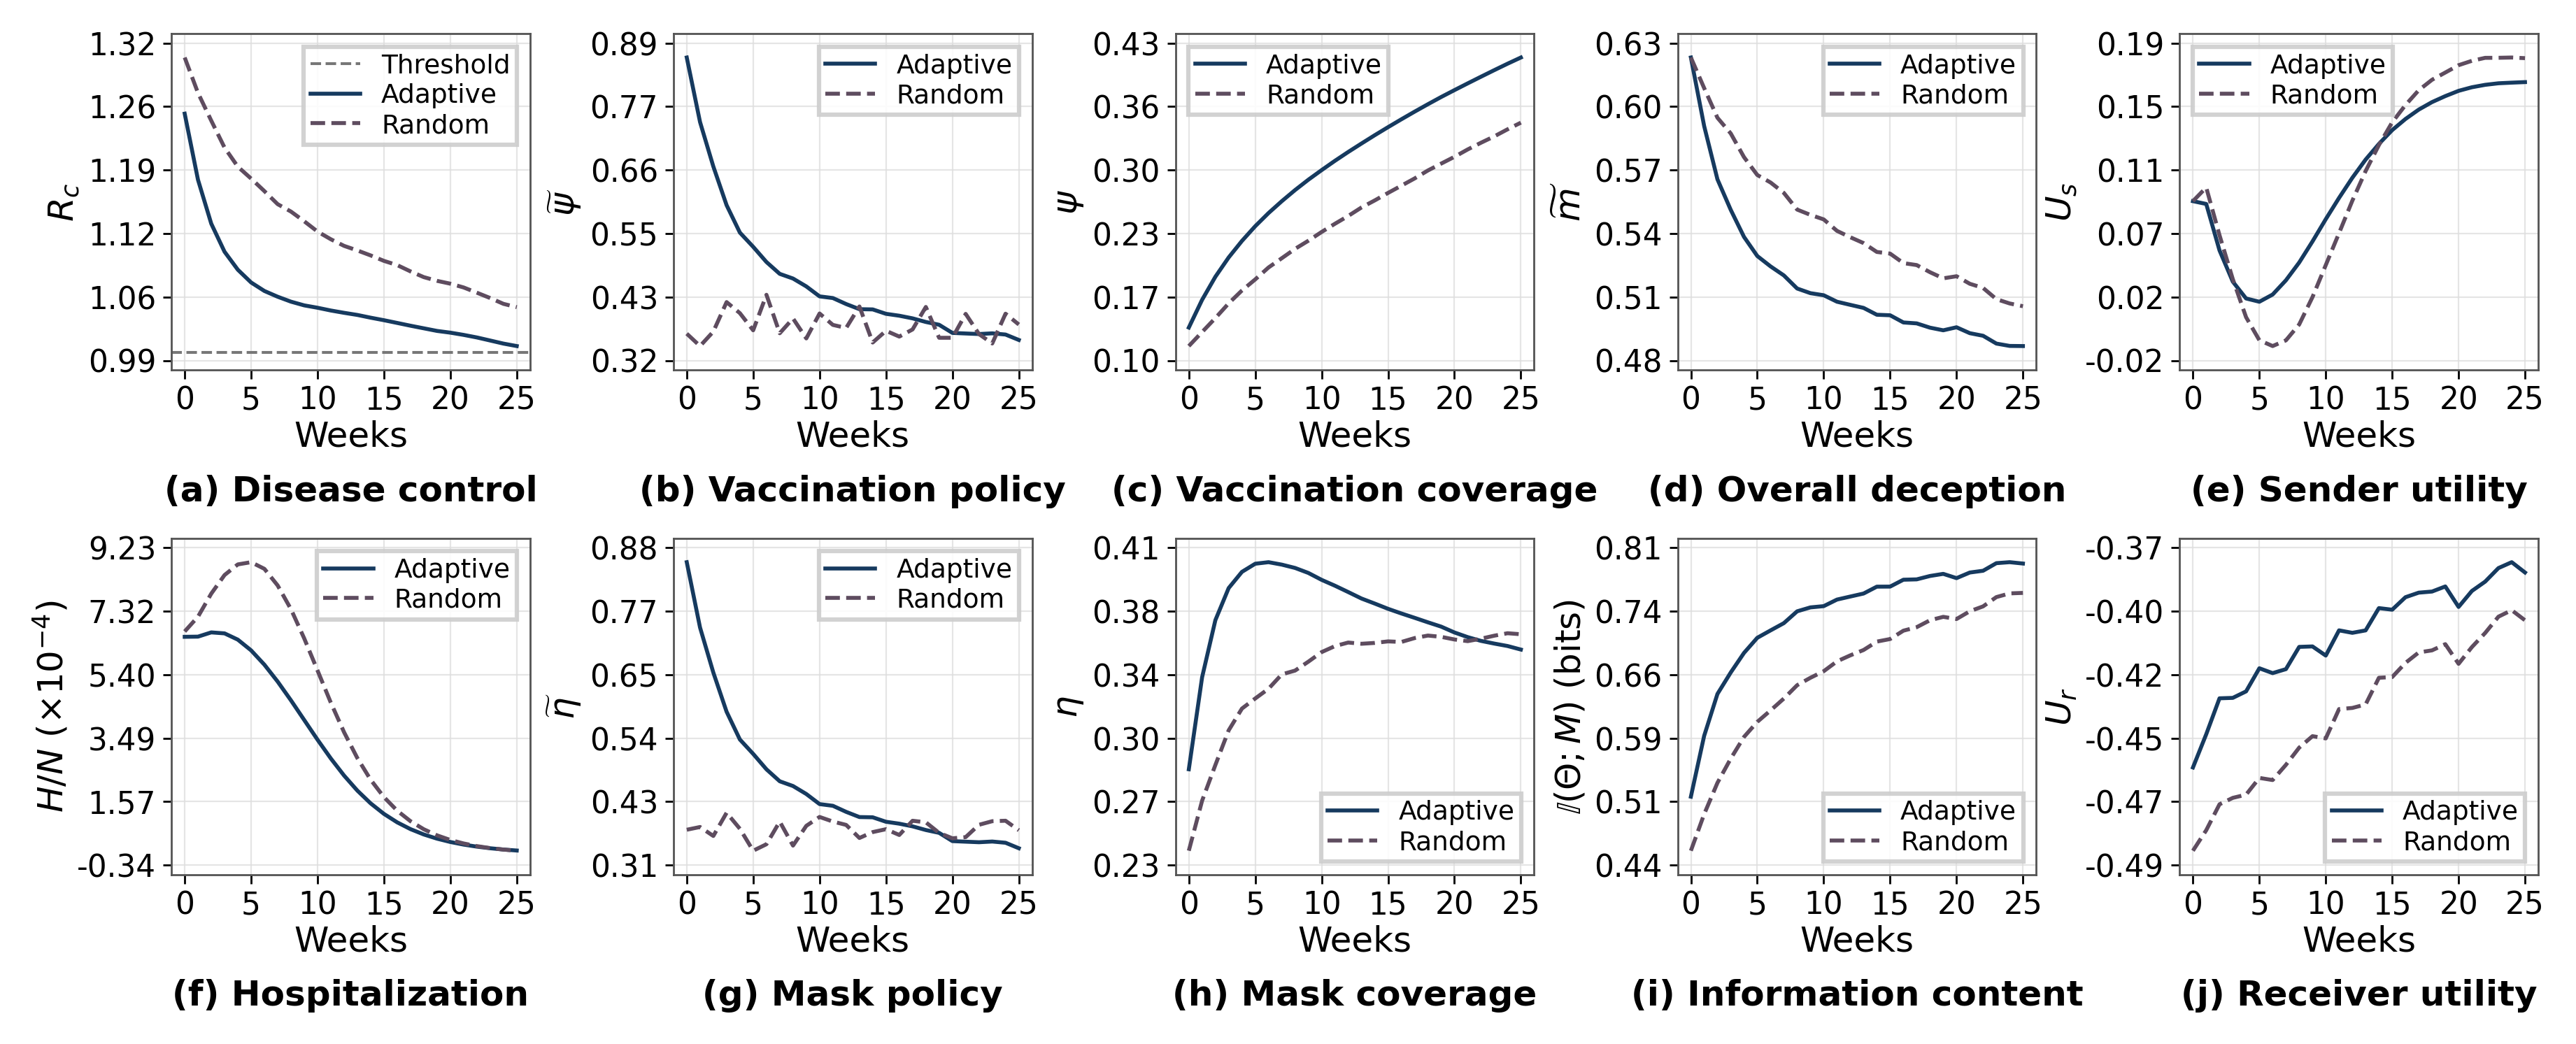
\includegraphics[width=\textwidth, height=4.7cm]{figures/policy_partial_pooling_high}
    \caption{Comparison of adaptive and random policies under partial pooling with high initial behavioral rates, across epidemic dynamics, policy actions, signaling behavior, and utilities.}
    \label{fig:policy_partial_high} %\vspace{-4mm}
\end{figure*}

\begin{figure*}[h]
    \centering
    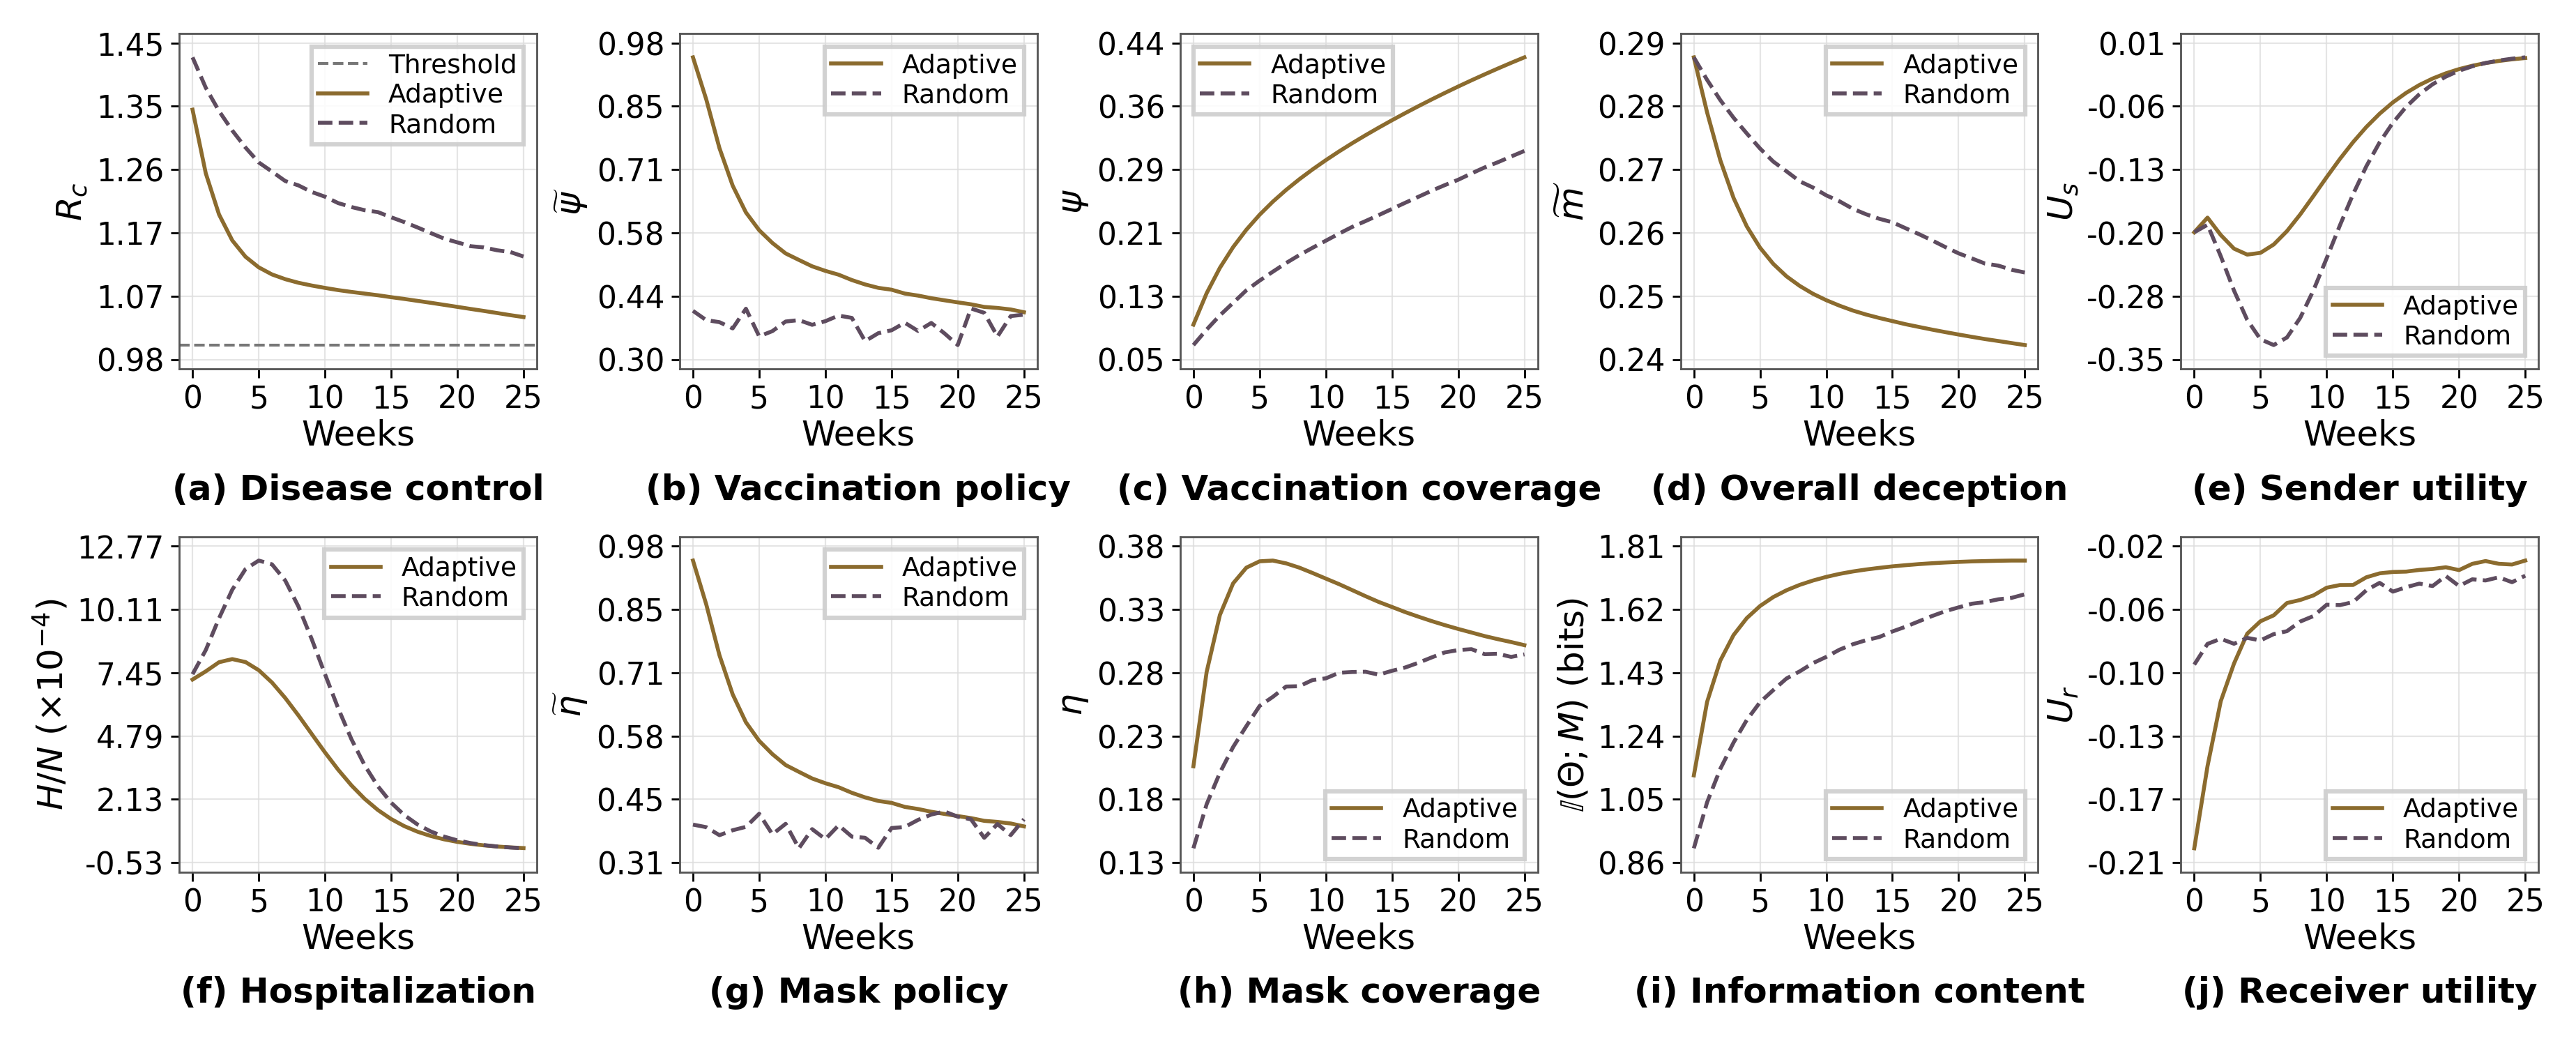
\includegraphics[width=\textwidth, height=4.7cm]{figures/policy_separating_low.png}
    \caption{Comparison of adaptive and random policies under separating with low initial behavioral rates, across epidemic dynamics, policy actions, signaling behavior, and utilities.}
    \label{fig:policy_sep_low} %\vspace{-4mm}
\end{figure*}

\begin{figure*}[h]
    \centering
    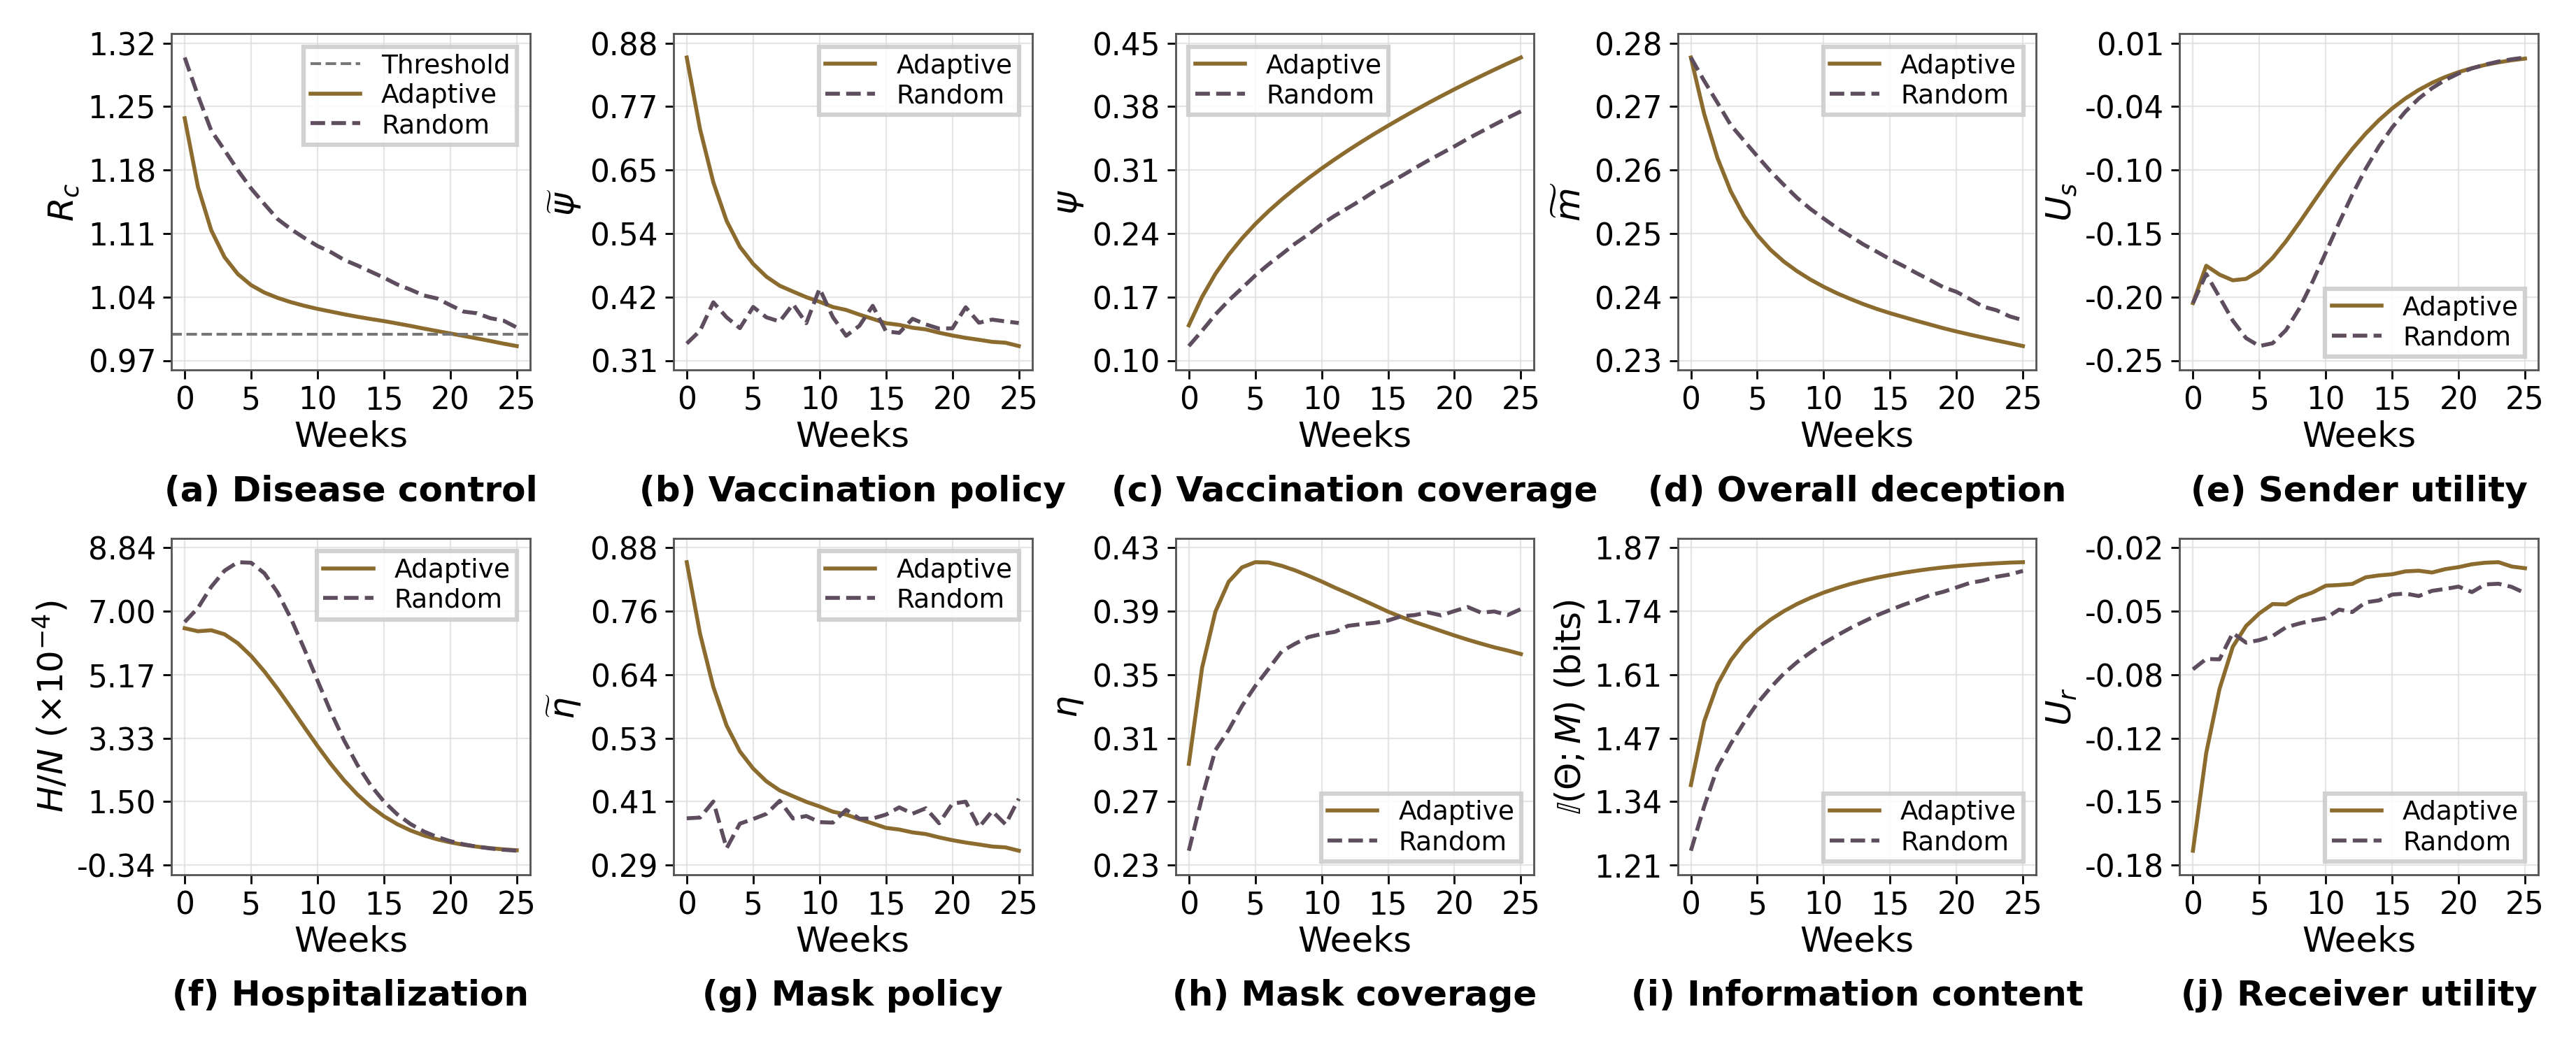
\includegraphics[width=\textwidth, height=4.7cm]{figures/policy_separating_high.png}
    \caption{Comparison of adaptive and random policies under separating with high initial behavioral rates, across epidemic dynamics, policy actions, signaling behavior, and utilities.}
    \label{fig:policy_sep_high} %\vspace{-4mm}
\end{figure*}

\begin{figure*}[h]
    \centering
    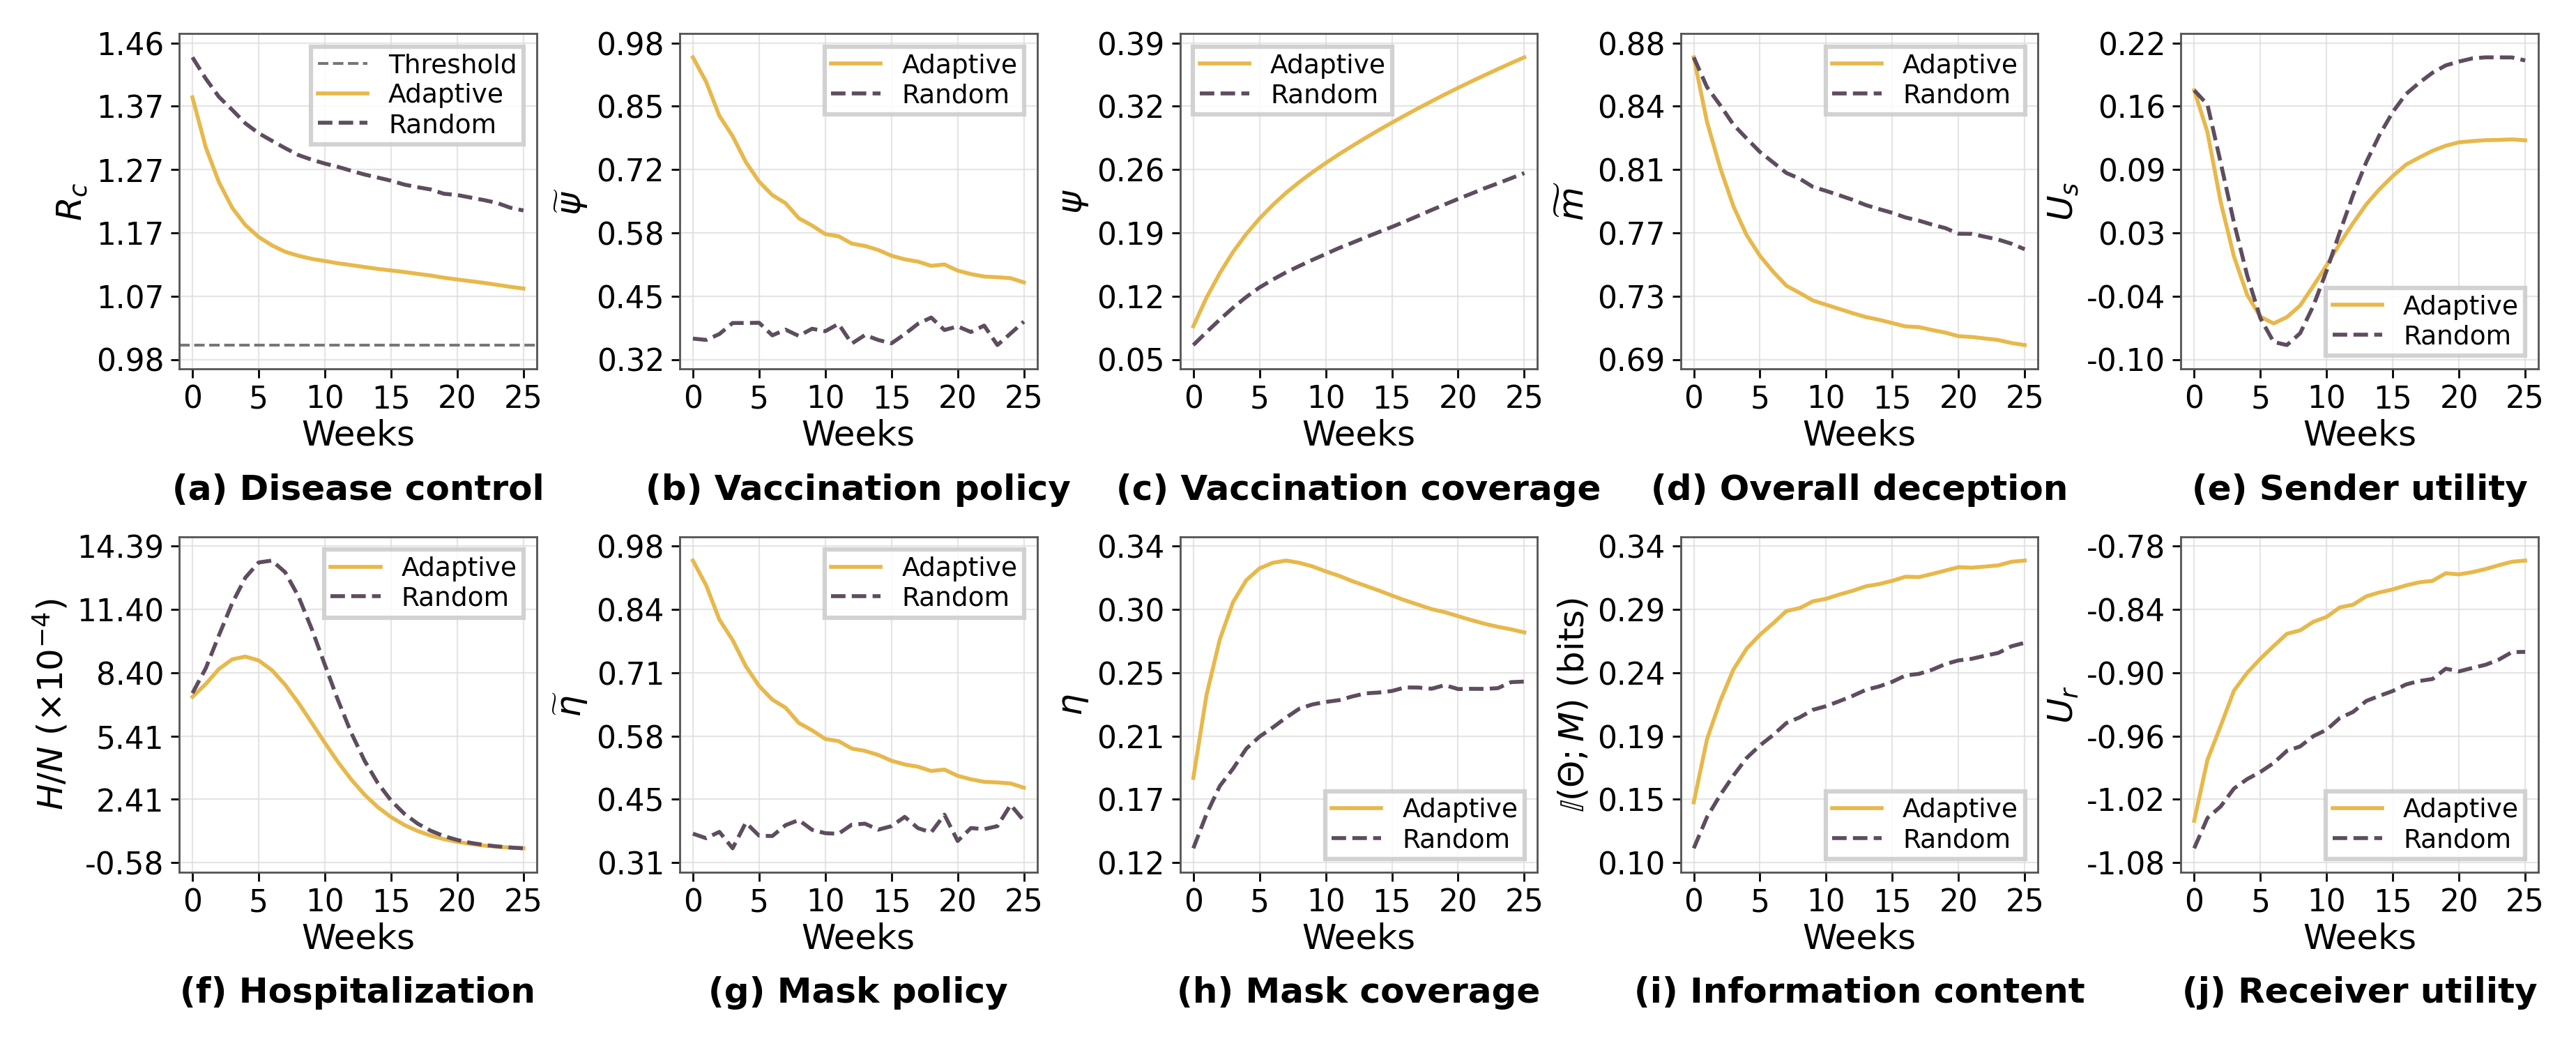
\includegraphics[width=\textwidth, height=4.7cm]{figures/policy_pooling_low.png}
    \caption{Comparison of adaptive and random policies under pooling with low initial behavioral rates, across epidemic dynamics, policy actions, signaling behavior, and utilities.}
    \label{fig:policy_pool_low} %\vspace{-4mm}
\end{figure*}

\begin{figure*}[h]
    \centering
    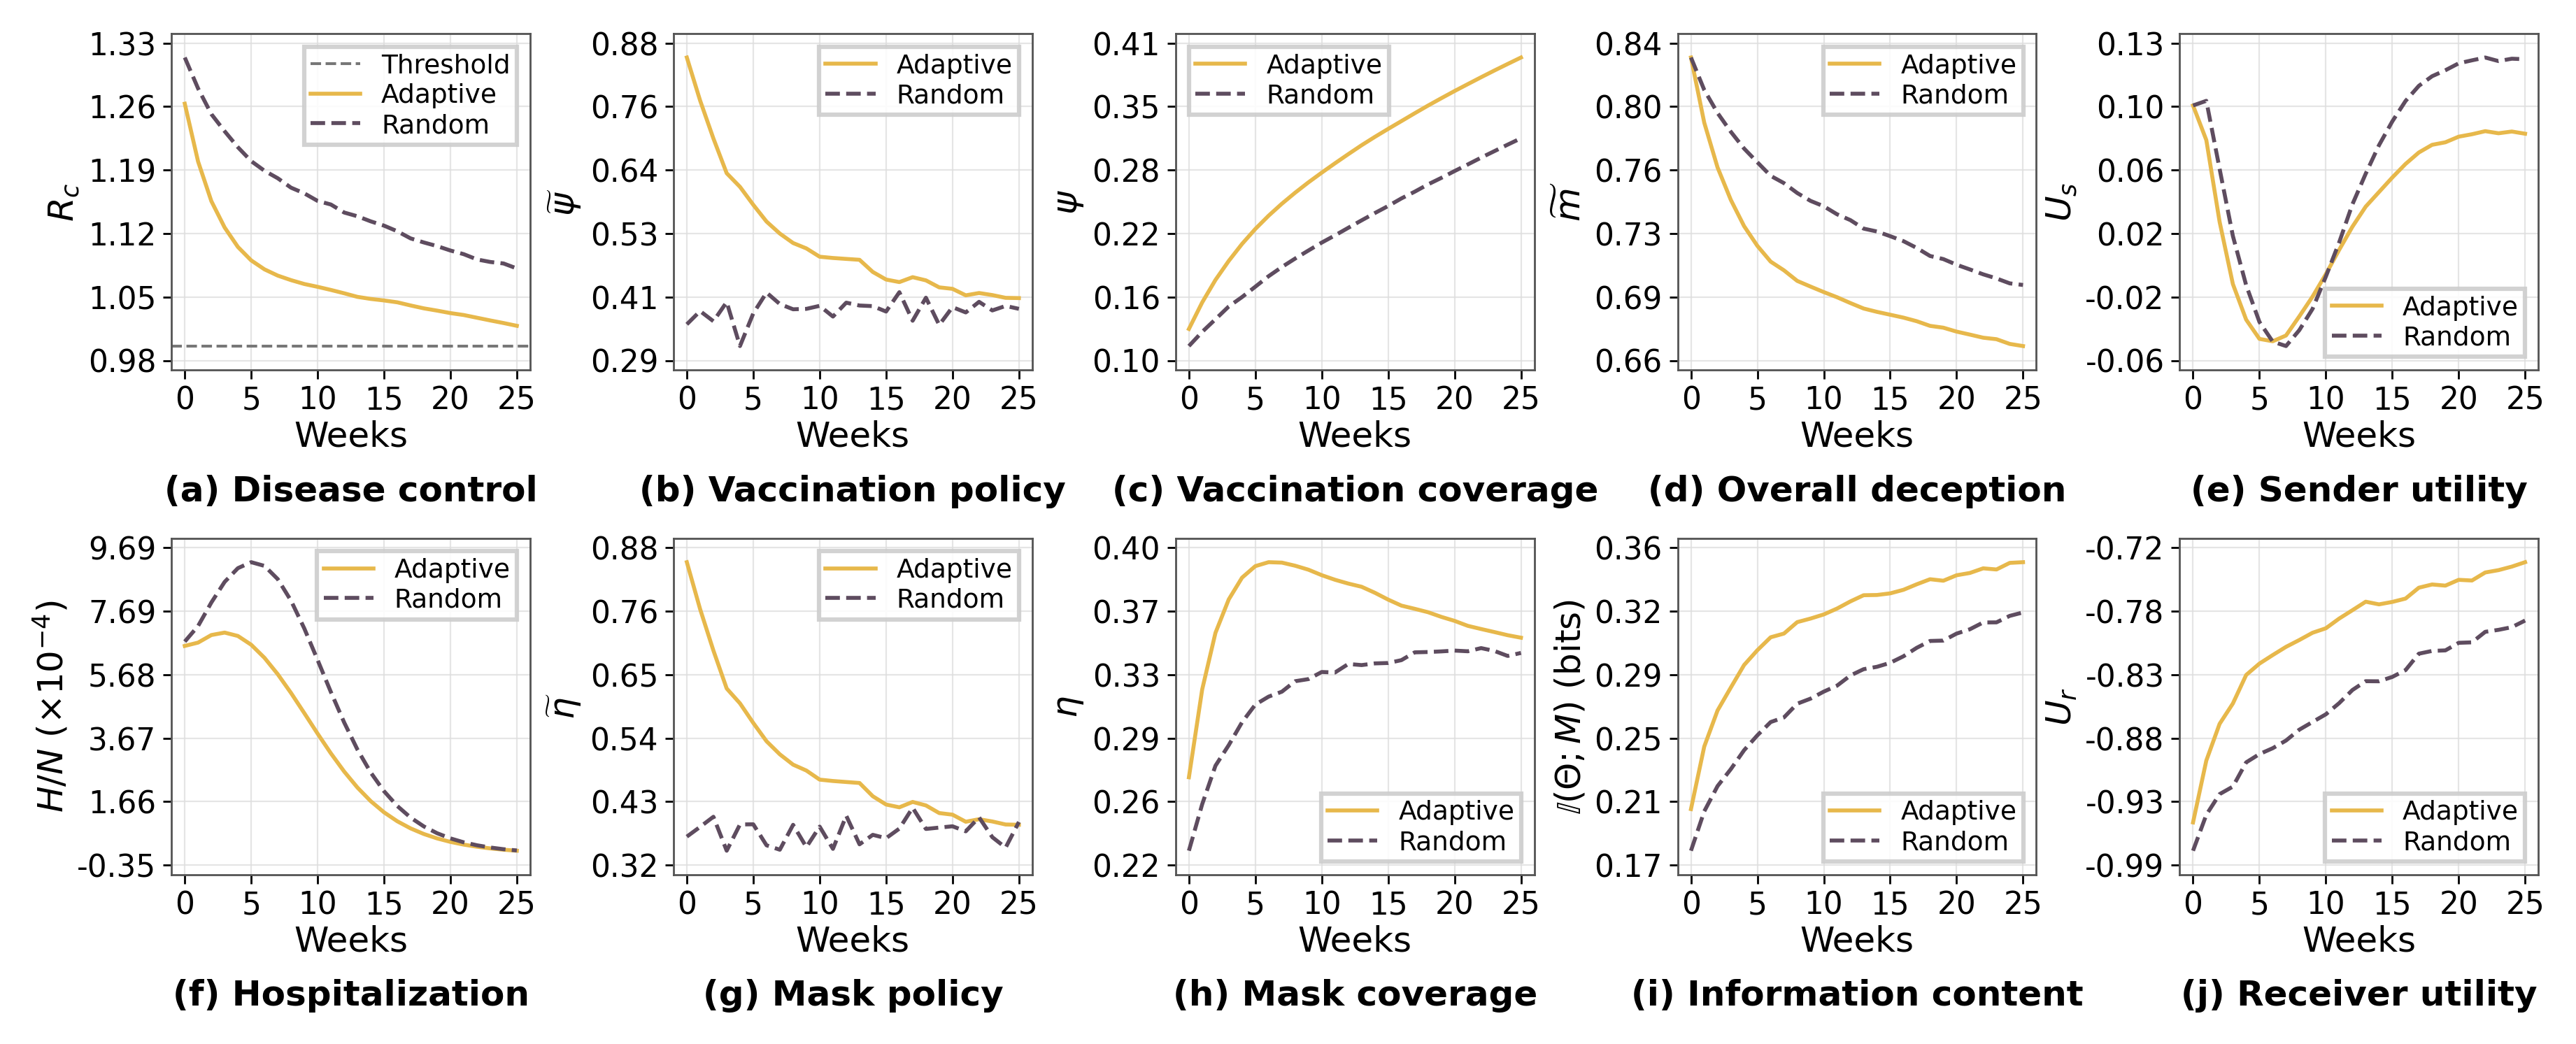
\includegraphics[width=\textwidth, height=4.7cm]{figures/policy_pooling_high.png}
    \caption{Comparison of adaptive and random policies under pooling with high initial behavioral rates, across epidemic dynamics, policy actions, signaling behavior, and utilities.}
    \label{fig:policy_pool_high} %\vspace{-4mm}
\end{figure*}



\subsection{Component-level evidence on false signals and receiver response}
\label{supp:indirect-evidence}

The framework assumes two things about the environment in which reporting happens: that
false content is a real and unevenly distributed feature of it, and that receivers respond
to signals in a way that interventions can shift. Neither assumption is testable on the
CTIS--CDC panel, which observes aggregate coverage rather than individual messages, so we
examine them separately on three corpora, reported in Figure~\ref{fig:indirect_evidence}.

Two patterns bear on the sender side. Exposure to verified-false COVID-19 content is
highly concentrated (Figure~\ref{fig:indirect_evidence}a): the Gini coefficient of
per-item engagement is $0.84$ over 332 fact-checked Weibo posts with 26{,}501 timestamped
receiver actions (CHECKED) and $0.78$ over 166 fact-checked English-language items
(CoAID). Values near one mean exposure is dominated by a small minority of items rather
than spread uniformly. Amplification also precedes deliberation
(Figure~\ref{fig:indirect_evidence}b): reposts of verified-false CHECKED posts arrive at a
median $7.8$\,h after publication against $13.6$\,h for comments ($p<10^{-50}$), a gap of
roughly six hours during which a false signal propagates before it is discussed. Both are
consistent with a setting in which misreporting is structured rather than idiosyncratic,
which is the premise the sender model encodes.

The third result bears on the receiver side, and it is a partial negative that we report
as such (Figure~\ref{fig:indirect_evidence}c). In a randomised accuracy prime with 855
participants and 25{,}627 headline ratings, discernment, the difference between true- and
false-headline sharing, rose by $+0.034$ $[0.014, 0.055]$. It did so by increasing
true-content sharing $+0.036$ $[-0.004, 0.075]$ rather than by reducing false-content
sharing $+0.001$ $[-0.040, 0.042]$. Receiver behaviour is therefore modifiable, which the
adaptive-feedback component requires, but the channel is not suppression of false signals.

\paragraph{What this evidence does and does not establish.}
These corpora speak to message veracity, diffusion structure and receiver
responsiveness. None of them observes an individual's true vaccination or masking status
alongside that same individual's report, so none validates the misreport channel
$g(m\mid\theta)$ directly, and none identifies strategic intent. They are component-level
support for the assumptions the framework makes about its environment, not evidence for
the framework itself. The direct test of $g(m\mid\theta)$ is the paired
report-versus-record analysis of Table~\ref{tab:nis-teen-validation}, and the end-to-end
test is the CTIS--CDC evaluation in the main text.

\begin{figure}[tbp]
\centering
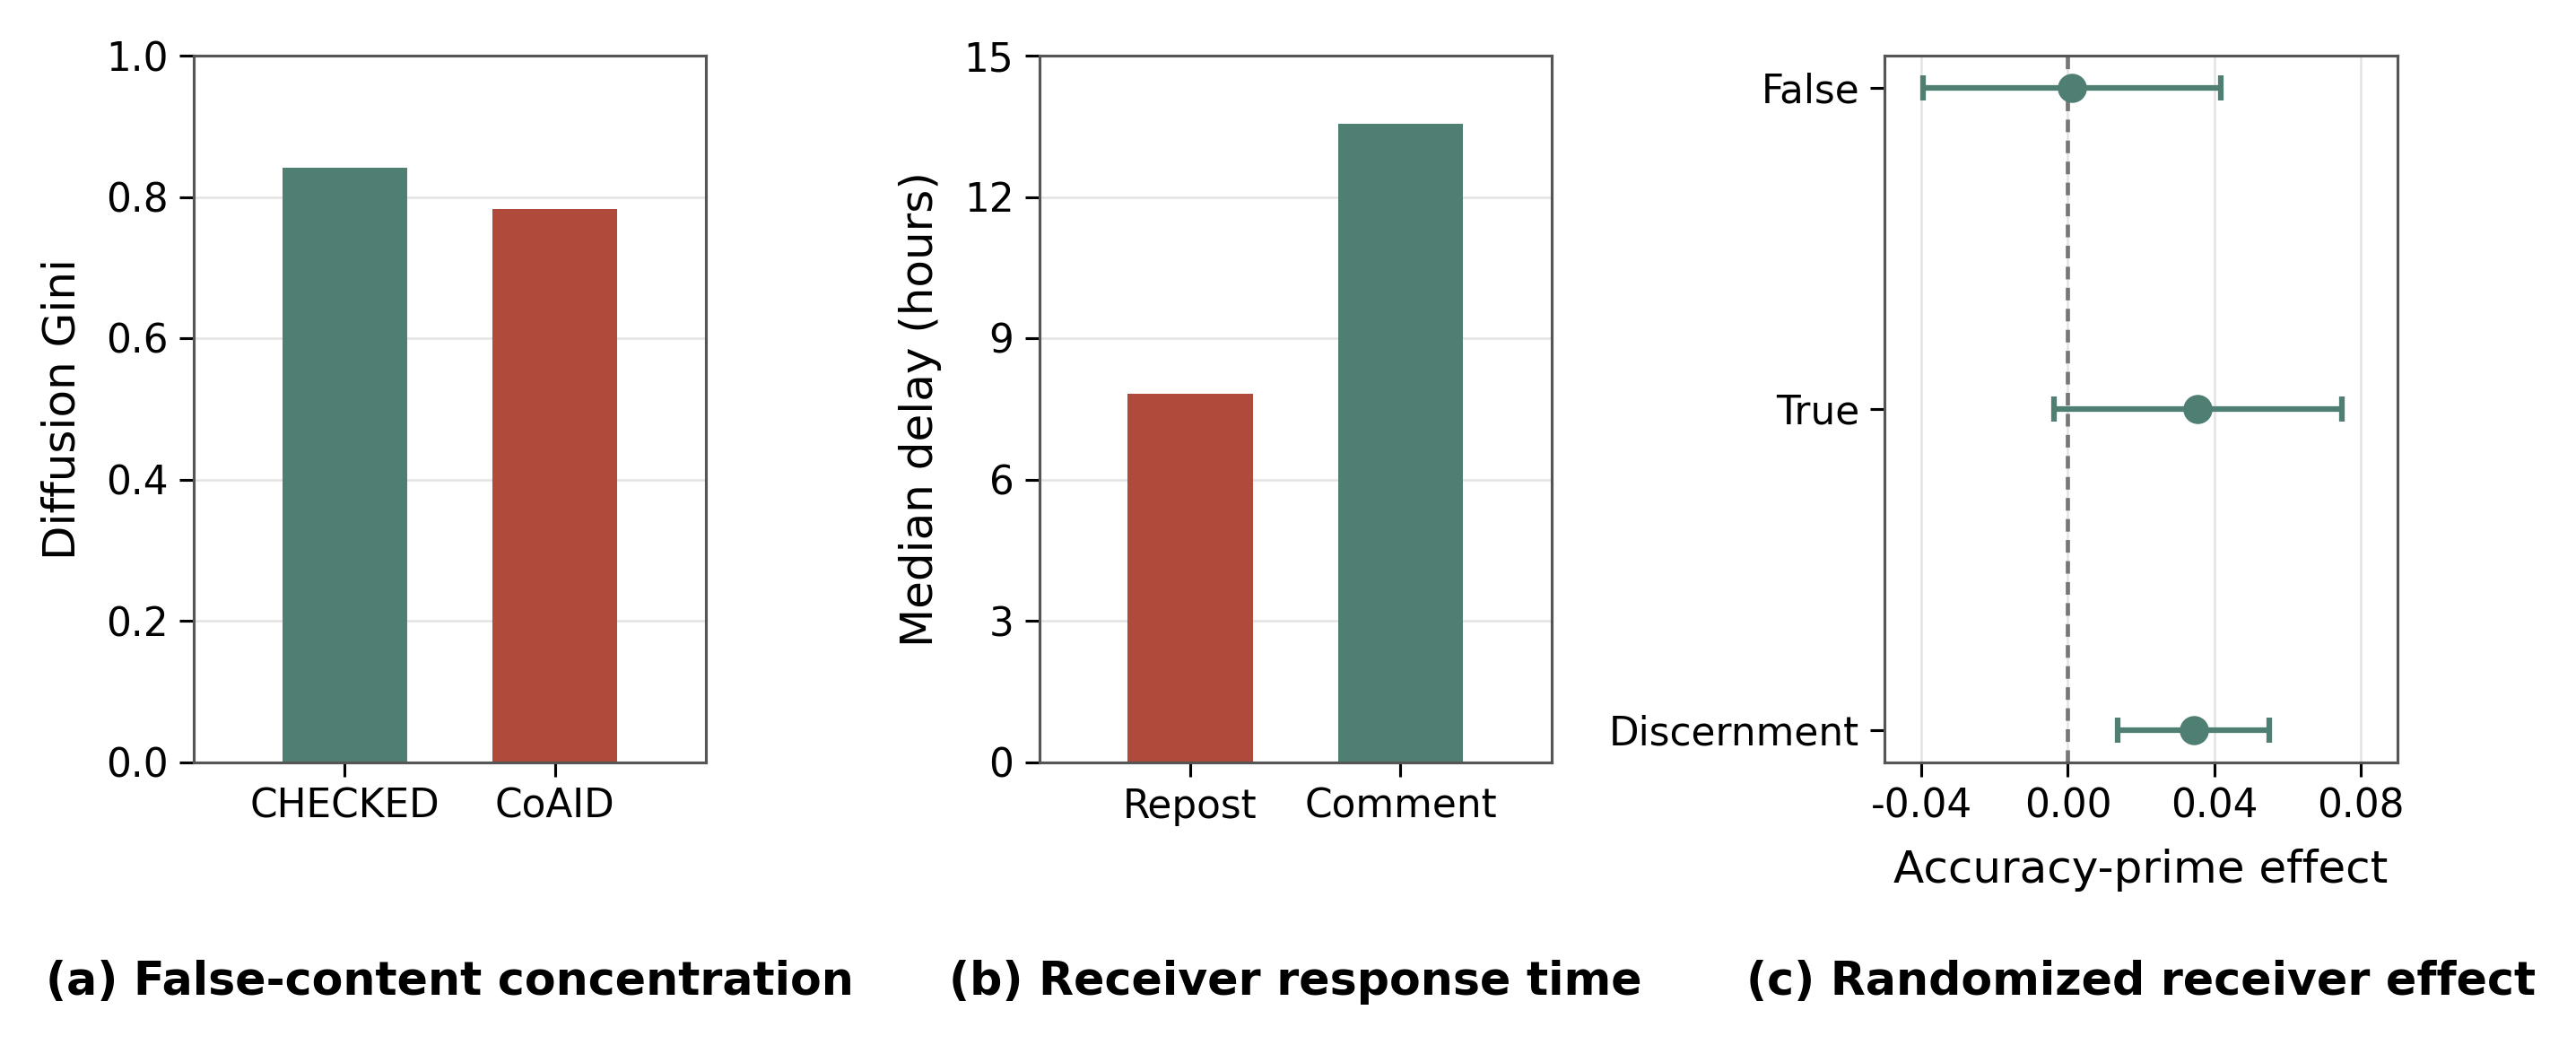
\includegraphics[width=\columnwidth]{figures/indirect_evidence.png}
\vspace{-5mm}
\caption{Component-level empirical evidence on false-signal diffusion and receiver
response. \textbf{(a)} Diffusion concentration. \textbf{(b)} Response latency.
\textbf{(c)} Accuracy prime.}
\label{fig:indirect_evidence}
\vspace{-4mm}
\end{figure}

\subsection{Deception patterns}

\begin{figure}[tbp]
    \centering
    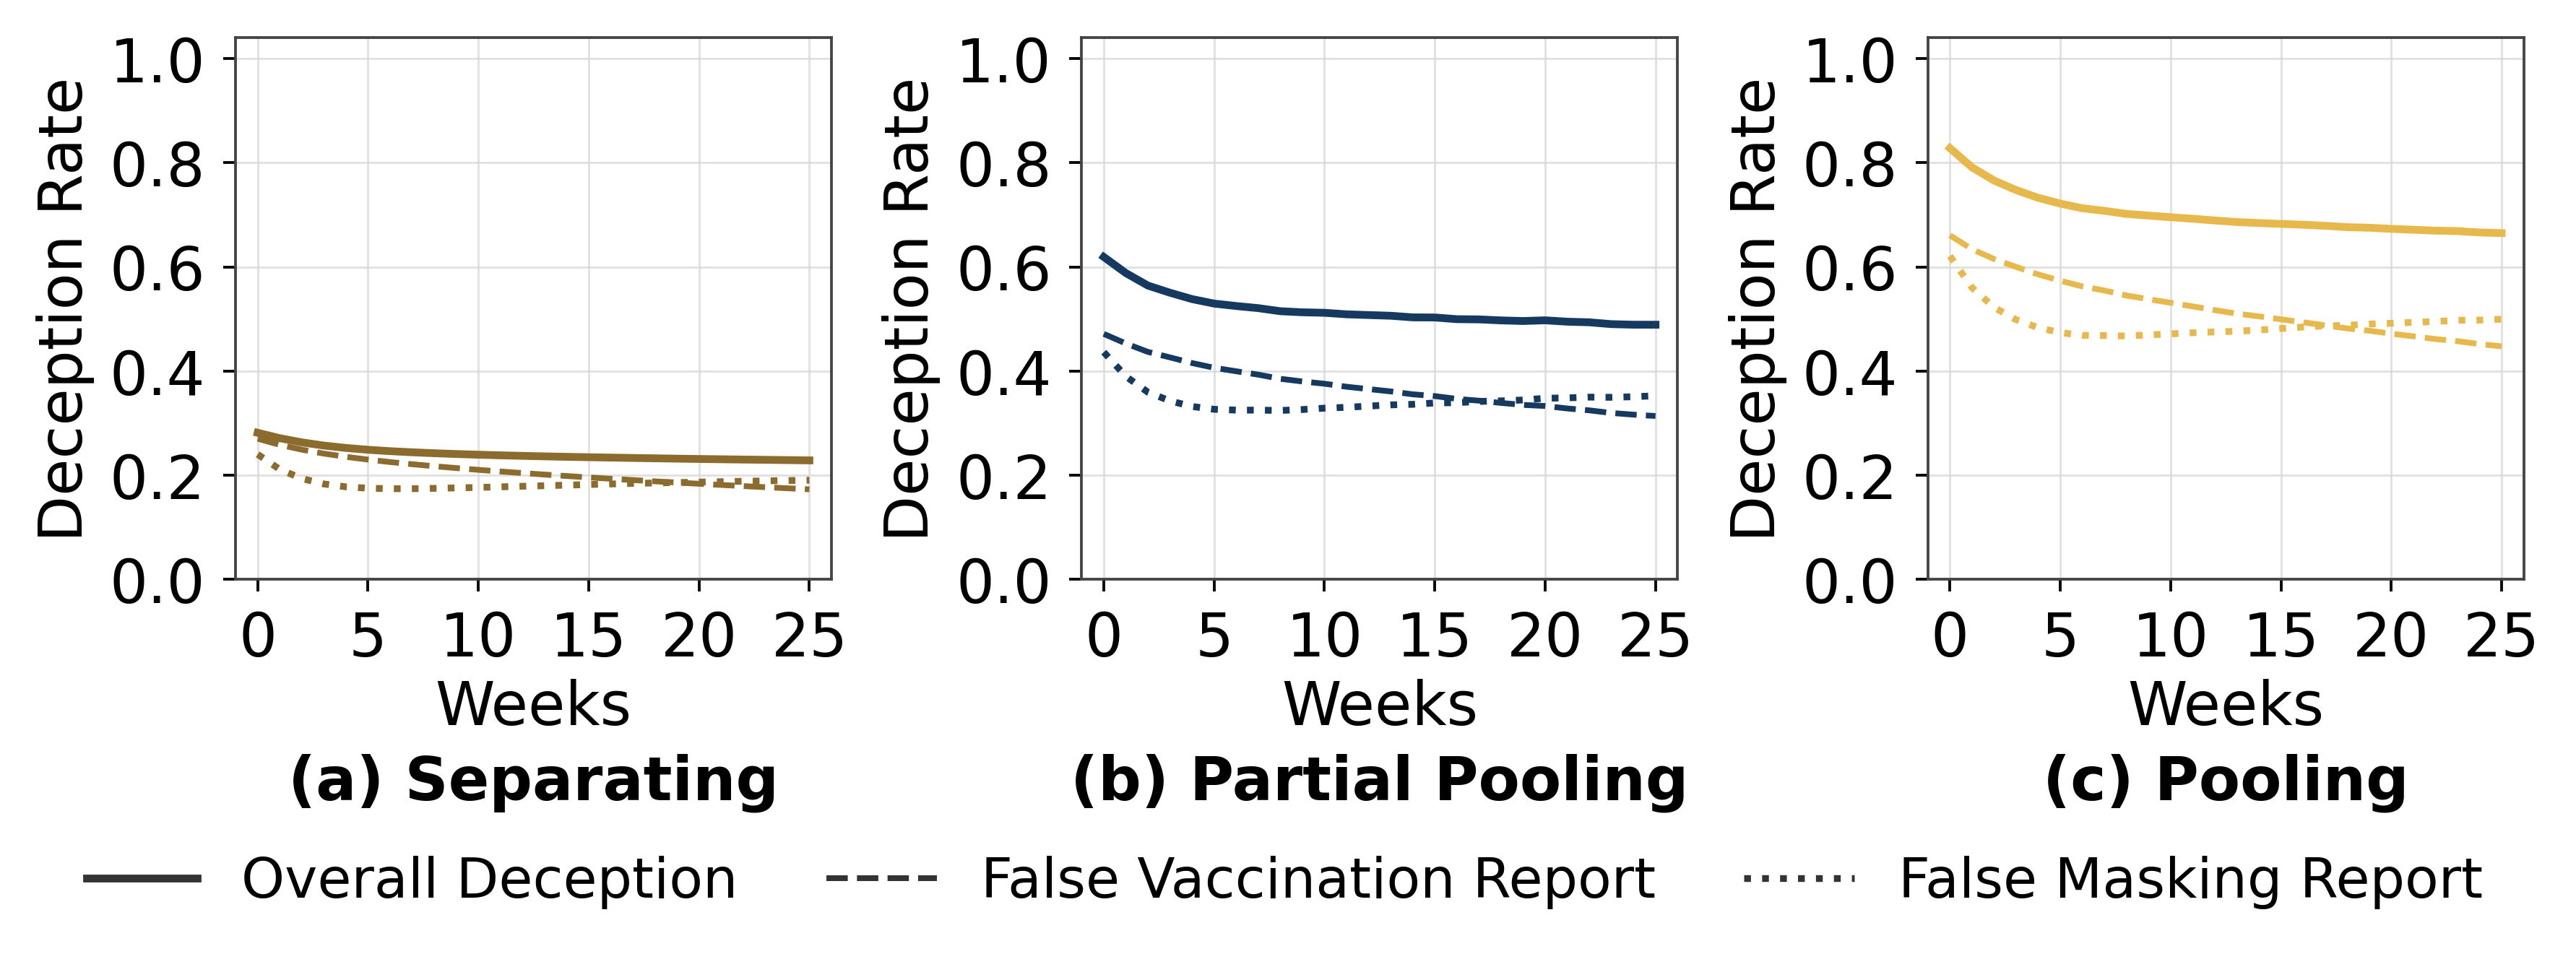
\includegraphics[width=\linewidth]{figures/deception_all-equilibria_high.png}
    \vspace{-4mm}
    \caption{The deception rates across equilibria under high initial behavioral rates.}
    \label{fig:deception_high}
    \vspace{-3mm}
\end{figure}

Figure~\ref{fig:deception_high}: The overall and separate strategy deception rates across equilibria under high initial behavioral rates.


Receiver sensitivity separates estimation from decision accuracy: moderate distortion regularization improves policy classification despite increasing coverage error (Table~\ref{tab:receiver-sensitivity}).

\begin{table}[tbp]
\centering
\caption{Sensitivity of the grid-based Bayesian receiver to
distortion regularization. Coverage error is in percentage
points; lower is better. This experiment is distinct from
the hierarchical estimator evaluated in
Figure~\ref{fig:real_case}.}
\label{tab:receiver-sensitivity}
\small
\setlength{\tabcolsep}{4pt}
\begin{tabular}{@{}rrrr@{}}
\toprule
$\lambda_2$
& \shortstack{Coverage\\error (pp)}
& $R_c$ error
& Policy error \\
\midrule
0.00 & \textbf{7.10} & \textbf{0.0420} & 0.1016 \\
0.25 & 7.30          & 0.0432          & \textbf{0.0967} \\
0.50 & 7.56          & 0.0447          & 0.0976 \\
1.00 & 8.24          & 0.0487          & 0.1222 \\
4.00 & 14.00         & 0.0828          & 0.2772 \\
\bottomrule
\end{tabular}
\end{table}


\paragraph{Paired report--record validation.} The 2021 CDC NIS-Teen links household-reported HPV vaccination to provider records for the same adolescent, excluding doses administered after the household interview. We use 16,708 paired observations, split into 11,695 training and 5,013 held-out observations. Analyses use provider survey weights. Intervals are obtained from 2,000 stratum-preserving household resamples with weights held fixed. All correction methods improve Brier score over raw reports, while differences among the correction methods are statistically indistinguishable. This evaluation measures reporting-error recovery rather than identification of strategic intent.

\begin{table}[tbp]
\centering
\caption{Paired individual validation on the 2021 NIS-Teen
held-out sample. Differences are weighted Brier scores
relative to raw household reports, with 95\% bootstrap
intervals. Lower is better.}
\label{tab:nis-teen-validation}
\small
\setlength{\tabcolsep}{3pt}
\renewcommand{\arraystretch}{1.02}
\begin{tabularx}{\columnwidth}{
@{}
>{\raggedright\arraybackslash}X
r
>{\centering\arraybackslash}p{0.42\columnwidth}
@{}}
\toprule
Method & Brier score & Difference [95\% CI] \\
\midrule
Raw household report
& 0.1853 & Reference \\
Audit calibration
& 0.1260 & $-0.0593$ [$-0.0753$, $-0.0439$] \\
Covariate logistic
& 0.1260 & $-0.0593$ [$-0.0755$, $-0.0435$] \\
Reporting channel
& 0.1261 & $-0.0593$ [$-0.0756$, $-0.0435$] \\
\bottomrule
\end{tabularx}
\end{table}


Structured correction includes contextual features and county adjustments. Its replacement by report-only calibration therefore tests the full correction structure, rather than the marginal contribution of incentive features. Removing consistency omits the county-wise monotone projection during inference while retaining the common evaluation mapping.

% \subsection{Stress test}

% \begin{figure}[htbp]
%     \centering
%     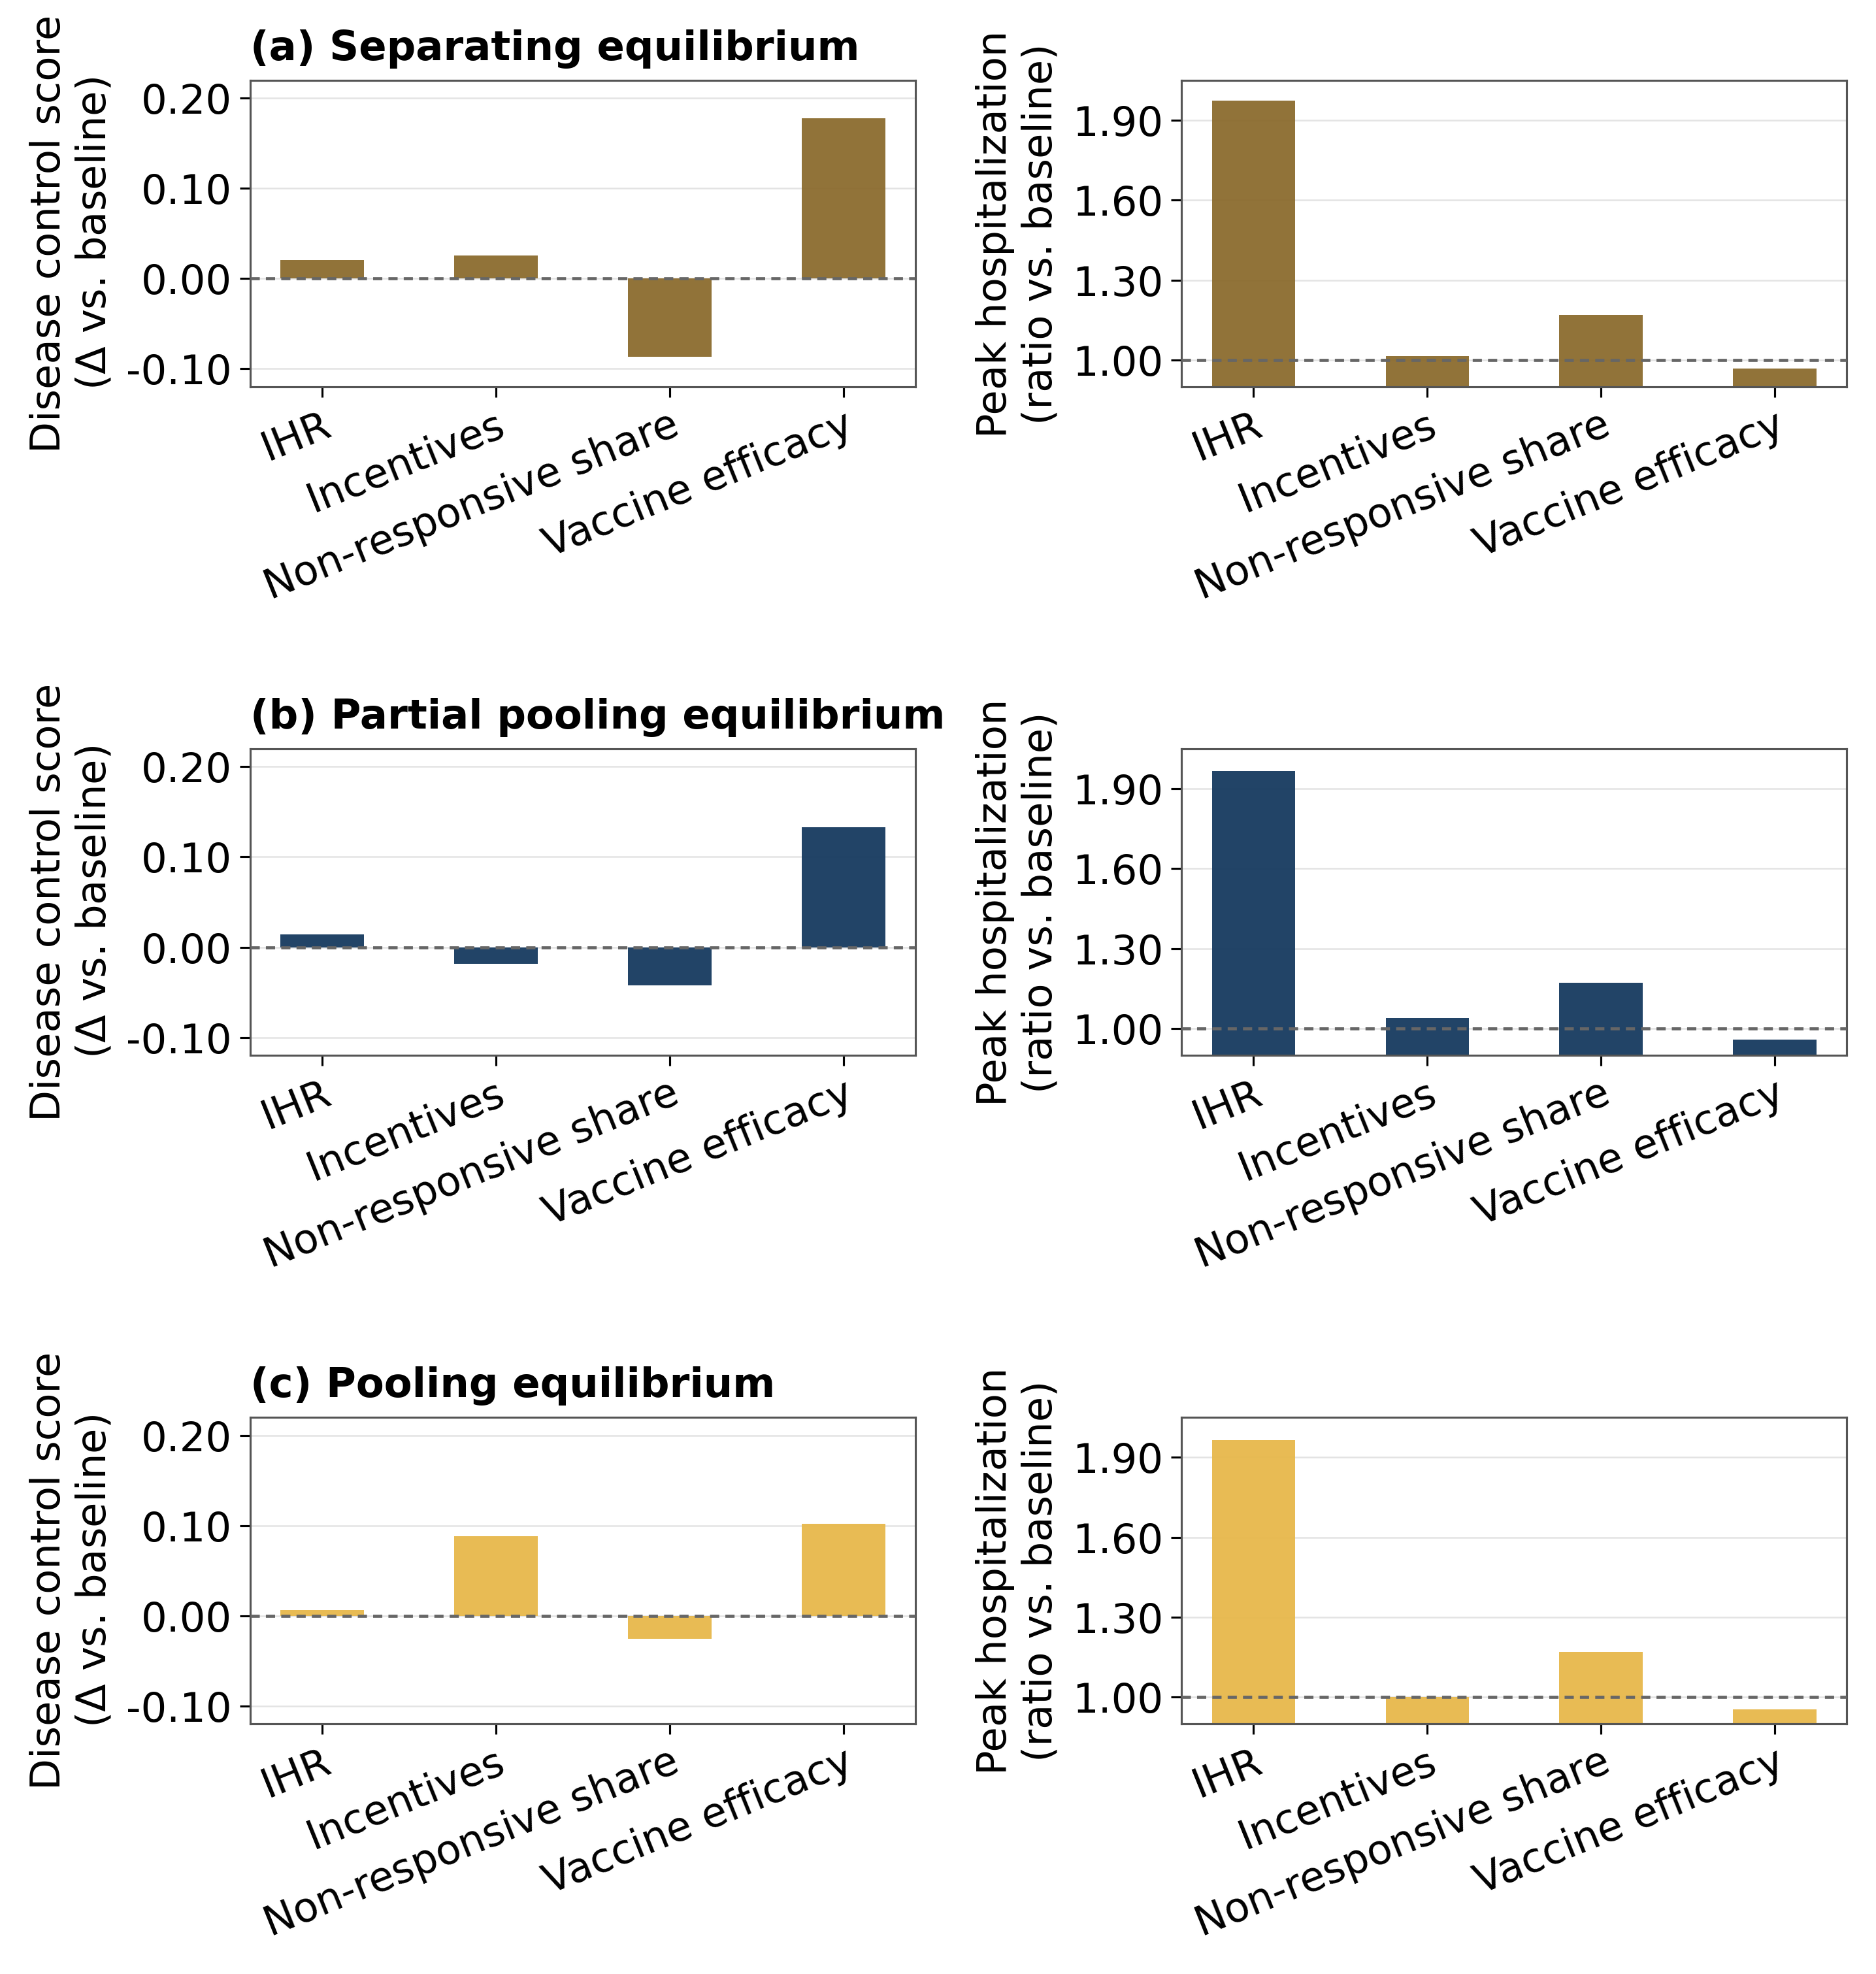
\includegraphics[width=\columnwidth]{figures/stress_summary.png}
%     \caption{Sensitivity of epidemic outcomes to stress factors across equilibria.}
%     \label{fig:stress}
% \end{figure}  


% Figure~\ref{fig:stress}: Sensitivity of epidemic outcomes to stress factors across equilibria.










% \bibliographystyle{ACM-Reference-Format}
% \bibliography{signaling_games}


\end{document}
\endinput
%%
%% End of file `sigconf.tex'.
